\documentclass[10pt,aspectratio=169,xcolor={table,xcdraw}]{beamer}

\usetheme[
%url={nano.polymtl.ca},
%numbering={false},
menuwidth={0.35\paperwidth}
]{polymtl}
\usepackage[utf8]{inputenc}
%\setlist[myitemize,1]{label=\textbullet,leftmargin=1in}
\setbeamercovered{transparent=20}
\usepackage{graphicx} 
\usepackage[table,xcdraw]{xcolor}
\graphicspath{{./Figures/}}
%\usepackage{epstopdf}
\usepackage{caption}
\usepackage[labelformat=simple]{subcaption}
\usepackage{multicol}
\usepackage{gensymb}
\usepackage{tabu}
\usepackage{xcolor}
\usepackage{siunitx}
\usepackage{booktabs}
\usepackage{float}
%\usepackage{subfigure}
\usepackage{ragged2e}
\usepackage{amsfonts}
\usepackage{cancel}
\usepackage{animate}
\usepackage{bm}
\usepackage{amsmath}
\usepackage{framed, color}
\usepackage{tcolorbox}
\usepackage{listings}
\usepackage[pangram]{blindtext}
\usepackage{lipsum}
\usepackage{tikz}
\usepackage{verbatim}
%\usepackage{pgfplots}
\usetikzlibrary{shapes,arrows,calc,shadows}
%\usetikzlibrary{decorations.markings}
\usepackage{pgfplots}
\usepackage{pgffor}
\usepackage{pgfgantt}
\bibliographystyle{unsrt}
\usepackage{amssymb}% http://ctan.org/pkg/amssymb
\usepackage{pifont}% http://ctan.org/pkg/pifont
\usepackage{sidecap}
\usepackage{wrapfig}

\usepackage[bottom]{footmisc}

%\usepackage{booktabs} 
\usepackage[]{algorithmicx}
\usepackage[]{algpseudocode}
\bibliographystyle{plain}
\usepackage{setspace}
\usepackage{marvosym} % \MVRIGHTarrow


\setbeamersize{text margin left=10pt,text margin right=10pt}
\setbeamertemplate{bibliography item}{\insertbiblabel}


\definecolor{shadecolor}{rgb}{0., 0., 0.}

\newcommand\topicSlide[3]{
\begin{frame}
\vspace*{1cm}
\begin{tcolorbox}[width=\textwidth,
boxsep=0pt,
left=0pt,
right=0pt,
top=10pt,
arc=0pt,
boxrule=0pt,toprule=1pt,
bottomrule=1pt,
colback=polymtlbluel,
grow to left by=10mm,
grow to right by=10mm,
arc = 0mm
]%%
\centering
\textcolor{polymtlwhite}{\huge #1}
\vspace*{10pt}
\textcolor{polymtlwhite}{\\ \Large #2}
\vspace*{10pt}
\textcolor{polymtlwhite}{\\ \normalsize #3}
\end{tcolorbox}
\end{frame}
}

\newcommand*\circled[1]{\tikz[baseline=(char.base)]{
            \node[shape=circle,draw,inner sep=3pt] (char) {#1};}}


\setbeamertemplate{caption}[numbered]
\captionsetup[figure]{labelformat=default}
\captionsetup[table]{labelformat=default}


\begin{document}

\title [IPW3 : ONERAM6]{\large IPW3 : ONERAM6 Code-to-Code Comparisons} 

\author[]{\small Karim Zayni, PhD Student \\ Maxime Blanchet, PhD Student \\ Éric Laurendeau, PhD, Professor}


\date{\small September 22, 2026}
\institute{Polytechnique Montreal}

\begin{frame}[plain]
\vspace{-0.5cm}
\begin{columns}
\column{.05\textwidth}
\column{.9\textwidth}
\titlepage
\column{.05\textwidth}
\end{columns}
\end{frame}

\begin{frame}{\small \textbf{Table of Contents}}
\small
\tableofcontents
\end{frame}

% ============================================================
% IPW3 -- Participants
% ============================================================

\begin{frame}{\small IPW3 -- Onera M6 Participants}
\scriptsize

% IPW3 participant colors
\definecolor{p001}{HTML}{2CA02C}
\definecolor{p002}{HTML}{17BECF}
\definecolor{p003}{HTML}{00695C}
\definecolor{p004}{HTML}{BCBD22}
\definecolor{p006}{HTML}{9467BD}
\definecolor{p007}{HTML}{1F77B4}
\definecolor{p008}{HTML}{D62728}
\definecolor{p009}{HTML}{A5006A}
\definecolor{p010}{HTML}{0047FF}
\definecolor{p013}{HTML}{637939}
\definecolor{p014}{HTML}{E377C2}
\definecolor{p015}{HTML}{393B79}
\definecolor{p019}{HTML}{E6550D}
\definecolor{p020}{HTML}{843C39}

\centering

\renewcommand{\arraystretch}{1.20}
\setlength{\tabcolsep}{8pt}

\begin{tabular}{ccc}
\toprule
\textbf{ID} &
\textbf{Participant / Organization} &
\textbf{Color} \\
\midrule

001 & CIRA                   & \textcolor{p001}{\rule{1.5cm}{1.5pt}} \\
002 & AeroTex                & \textcolor{p002}{\rule{1.5cm}{1.5pt}} \\
003 & NRC                    & \textcolor{p003}{\rule{1.5cm}{1.5pt}} \\
004 & ONERA                  & \textcolor{p004}{\rule{1.5cm}{1.5pt}} \\
007 & Polytechnique Montréal & \textcolor{p007}{\rule{1.5cm}{1.5pt}} \\
010 & NASA                   & \textcolor{p010}{\rule{1.5cm}{1.5pt}} \\
015 & NIAR                   & \textcolor{p015}{\rule{1.5cm}{1.5pt}} \\
019 & Synopsys               & \textcolor{p019}{\rule{1.5cm}{1.5pt}} \\

\bottomrule
\end{tabular}

\end{frame}

\section[Case \& Submissions]{\textbf{Case Conditions \& Submission Summary}}

% ============================================================
% ONERA M6 -- Geometry and Aerodynamic Conditions
% ============================================================

\begin{frame}{\small Geometry and Aerodynamic Conditions}
\scriptsize

\begin{columns}[T,onlytextwidth]

%------------------------------------------------
\begin{column}{0.43\textwidth}
\centering
\begin{figure}
    \centering
    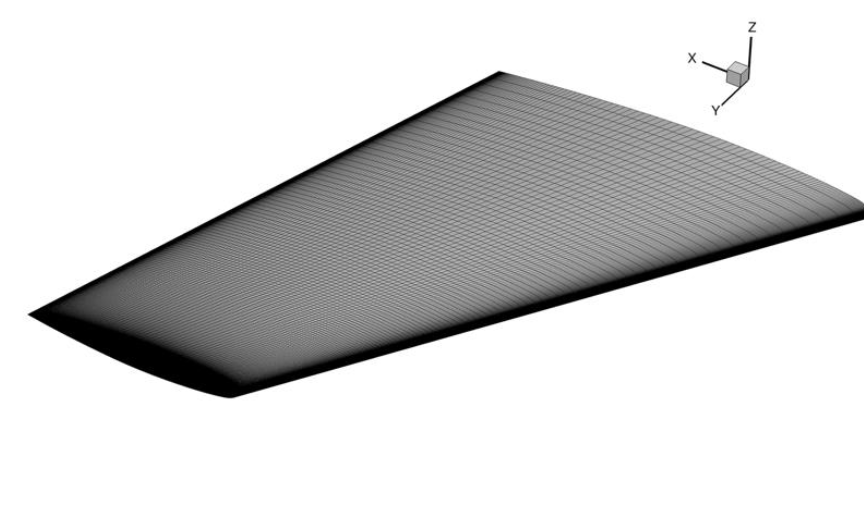
\includegraphics[height=0.6\textheight]{FIGURES_CONDITIONS/ONERA_M6_GEOMETRY_VIEW.png}
\end{figure}

\vspace{-0.15cm}

\centering
\textbf{ONERA M6 L1 Surface Mesh}

\end{column}

%------------------------------------------------
\begin{column}{0.53\textwidth}
\centering
\textbf{Geometry}

\vspace{0.15cm}

\begin{tabular}{lc}
\toprule
\textbf{Parameter} & \textbf{Value} \\
\midrule
Wing & ONERA M6 \\
Root chord [m] & $1.0$ \\
Semi-span [m] & $1.4760$ \\
Mean aerodynamic chord [m] & $0.801673$ \\
Reference area [m$^2$] & $1.1532$ \\
Angle of attack, $\alpha$ [$^\circ$] & $2.0$ \\
\bottomrule
\end{tabular}

\vspace{0.35cm}

\textbf{Aerodynamic Conditions}

\vspace{0.15cm}

\begin{tabular}{lc}
\toprule
\textbf{Parameter} & \textbf{Value} \\
\midrule
$M_\infty$ [-] & $0.40$ \\
$U_\infty$ [m/s] & $131.064$ \\
$T_\infty$ [K] & $267.15$ \\
$\rho_\infty$ [kg/m$^3$] & $0.68301$ \\
$Re_c$ [-] & $4.2558\times10^6$ \\
\bottomrule
\end{tabular}

\vspace{0.35cm}

\textbf{Quantities of Interest}

\vspace{-0.35cm}

\[
C_L,\qquad C_D,\qquad C_M,\qquad C_p
\]

\end{column}

\end{columns}

\end{frame}


% ============================================================
% ONERA M6 -- Icing Conditions
% ============================================================

\begin{frame}[shrink]{\small Icing Conditions}
\scriptsize

\begin{columns}[T,onlytextwidth]

%------------------------------------------------
\begin{column}{0.43\textwidth}
\centering
\begin{figure}
    \centering
    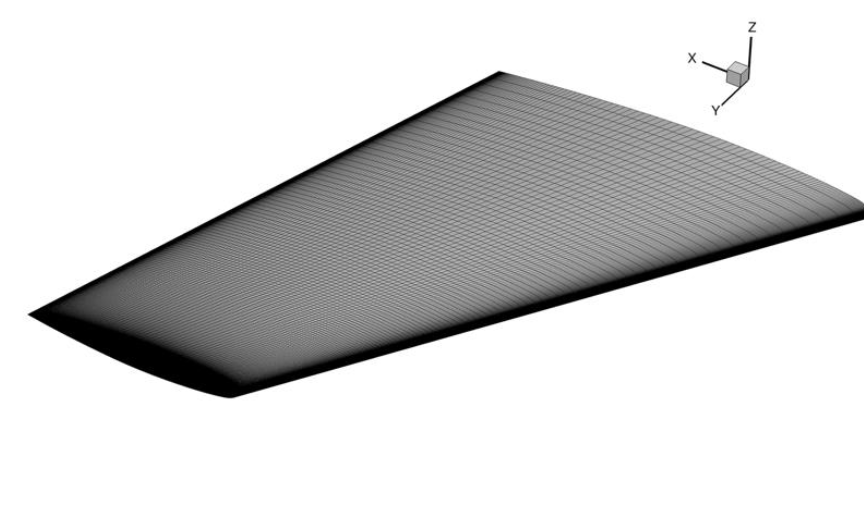
\includegraphics[height=0.6\textheight]{FIGURES_CONDITIONS/ONERA_M6_GEOMETRY_VIEW.png}
\end{figure}

\vspace{-1.0cm}

\textbf{ONERA M6 L1 Surface Mesh}

\vspace{0.20cm}

\centering
\begin{tabular}{lc}
\toprule
\textbf{Grid} & \textbf{Nodes} \\
\midrule
L1 & $60.78$ M \\
L2 & $7.63$ M \\
L3 & $0.960$ M \\
L4 & $0.122$ M \\
\bottomrule
\end{tabular}

\end{column}

%------------------------------------------------
\begin{column}{0.53\textwidth}
\centering
\textbf{Icing Conditions}

\vspace{0.15cm}

\begin{tabular}{lc}
\toprule
\textbf{Parameter} & \textbf{Value} \\
\midrule
$T_\infty$ [K]          & $267.15$ \\
$T_0$ [K]               & $275.7$ \\
$M_\infty$              & $0.40$ \\
$U_\infty$ [m/s]        & $131.064$ \\
LWC [g/m$^3$]           & $0.51$ \\
MVD [$\mu$m]            & $20$ \\
Exposure time [s]       & $1350$ \\
\bottomrule
\end{tabular}

\vspace{0.30cm}

\textbf{Droplet Distribution} : 1, 3, 7 $\&$ 15 bin distributions are considered

\vspace{0.25cm}

\begin{block}{\scriptsize Common Modeling Parameters}

A dimensional roughness of \textbf{$k_s=1.0$ mm} is prescribed as the baseline, and a common ice density of \textbf{$\rho_{\mathrm{ice}}=680~\mathrm{kg/m^3}$} is used for the comparison.

\end{block}

\vspace{0.35cm}

\textbf{Quantities of Interest}

\vspace{-0.35cm}

\[
\beta,\quad HTC,\quad T_s,\quad FF,\quad
m_{\mathrm{water}},\quad m_{\mathrm{ice}},\quad
m_{\mathrm{evap}}
\]

\end{column}

\end{columns}

\end{frame}

% ============================================================
% ONERA M6 -- Modeling Choices
% ============================================================

\begin{frame}{\small ONERA M6 -- Modeling Choices Across Submissions}
\scriptsize

\centering

\renewcommand{\arraystretch}{1.40}
\setlength{\tabcolsep}{2.2pt}

\begin{tabular}{c|ccccc}
\toprule
\textbf{Model / Method}
& \textbf{001}
& \textbf{002}
& \textbf{004}
& \textbf{007}
& \textbf{019} \\
\midrule

\textbf{Turbulence}
& $k$--$\omega$ TNT
& $k$--$\omega$ SST
& $k$--$\omega$ SST
& SA
& $k$--$\omega$ SST \\

\textbf{Droplet formulation}
& Eul.
& Lag.
& Eul.
& Eul.
& Eul. \\

\textbf{HTC method}
& --
& BL Int.
& $T_{rec}$
& $T_{rec}$
& -- \\

\textbf{Thermodynamics}
& Mess.
& Mess.
& Mess.
& Mess.
& SWIM+ \\

\textbf{Geometry evolution}
& Lag./IB
& Interp.
& --
& Lag.
& Lag./remesh \\

\textbf{No. of shots}
& $1$ / Multi
& $1$
& $1$
& $1$
& Multi \\

\bottomrule
\end{tabular}%


\vspace{0.12cm}

\begin{minipage}{0.98\textwidth}
\tiny
\textit{
Eul. = Eulerian;
Lag. = Lagrangian;
SA = Spalart--Allmaras;
BL Int. = boundary-layer integral;
$T_{rec}$ = recovery temperature;
Mess. = Messinger;
SWIM = shallow-water icing model;
IB = immersed boundary;
ALE = arbitrary Lagrangian--Eulerian;
Interp. = interpolation;
disp. = displacement;
Multi = multilayer/multishot;
-- = not reported.
}
\end{minipage}

\vspace{0.10cm}

\begin{block}{\scriptsize Overall Trends}
\begin{itemize}
    \item $k$--$\omega$ SST and Eulerian droplet formulations are the predominant choices among the disclosed submissions.
    \item Thermodynamic modeling is predominantly Messinger-based, while geometry-evolution methods are more diverse.
    \item Both single-shot and multishot strategies are represented.
\end{itemize}
\end{block}

\end{frame}

% ============================================================
% ONERA M6 -- Data Received
% ============================================================

\begin{frame}{\small ONERA M6 -- Summary of Data Received}
\scriptsize

\centering

\renewcommand{\arraystretch}{1.15}
\setlength{\tabcolsep}{3.5pt}

\begin{tabular}{c|cccc|cccc|cccc|cccc}
\toprule
&
\multicolumn{4}{c|}{\textbf{L1}} &
\multicolumn{4}{c|}{\textbf{L2}} &
\multicolumn{4}{c|}{\textbf{L3}} &
\multicolumn{4}{c}{\textbf{L4}} \\

\textbf{ID}
& 1 & 3 & 7 & 15
& 1 & 3 & 7 & 15
& 1 & 3 & 7 & 15
& 1 & 3 & 7 & 15 \\
\midrule

001 & \checkmark&&& & \checkmark&\checkmark&\checkmark&\checkmark & \checkmark&\checkmark&\checkmark&\checkmark & \checkmark&\checkmark&\checkmark&\checkmark \\

002 & \checkmark&\checkmark&\checkmark&\checkmark & \checkmark&\checkmark&\checkmark&\checkmark & \checkmark&\checkmark&\checkmark&\checkmark & \checkmark&\checkmark&\checkmark&\checkmark \\

003 & &&& & \multicolumn{4}{c|}{$*$} & \multicolumn{4}{c|}{$*$} & \multicolumn{4}{c}{$*$} \\

004 & \checkmark&\checkmark&\checkmark&\checkmark & \checkmark&\checkmark&\checkmark&\checkmark & \checkmark&\checkmark&\checkmark&\checkmark & \checkmark&\checkmark&\checkmark&\checkmark \\

007 & \checkmark&\checkmark&\checkmark&\checkmark & \checkmark&\checkmark&\checkmark&\checkmark & \checkmark&\checkmark&\checkmark&\checkmark & \checkmark&\checkmark&\checkmark&\checkmark \\

010 & \checkmark&\checkmark&\checkmark&\checkmark & \checkmark&\checkmark&\checkmark&\checkmark & \checkmark&\checkmark&\checkmark&\checkmark & \checkmark&\checkmark&\checkmark&\checkmark \\

015 & \checkmark&\checkmark&\checkmark&\checkmark & \checkmark&\checkmark&\checkmark&\checkmark & \checkmark&\checkmark&\checkmark&\checkmark & \checkmark&\checkmark&\checkmark&\checkmark \\

019 & \checkmark&\checkmark&\checkmark&\checkmark & \checkmark&\checkmark&\checkmark&\checkmark & \checkmark&\checkmark&\checkmark&\checkmark & \checkmark&\checkmark&\checkmark&\checkmark \\

\midrule
\textbf{Total}
& \textbf{7} & \textbf{6} & \textbf{6} & \textbf{6}
& \textbf{7} & \textbf{7} & \textbf{7} & \textbf{7}
& \textbf{7} & \textbf{7} & \textbf{7} & \textbf{7}
& \textbf{7} & \textbf{7} & \textbf{7} & \textbf{7} \\
\bottomrule
\bottomrule
\end{tabular}

\vspace{0.15cm}


\parbox{0.95\textwidth}{\scriptsize\raggedright
\centering
\checkmark: populated CutData received for the corresponding droplet-bin distribution.
\\
$*$: Excel results only, no CutData slices.
}

\end{frame}
% ============================================================
% ============================================================
% ONERA M6 -- AERODYNAMIC GRID CONVERGENCE
% ============================================================
% ============================================================

\section[Aero.]{\textbf{Aerodynamic Grid Convergence}}


% ============================================================
% ONERA M6 -- Aerodynamic Grid Convergence: CL
% ============================================================

\begin{frame}{\small ONERA M6 -- Lift Coefficient Grid Convergence}
\scriptsize

{\centering
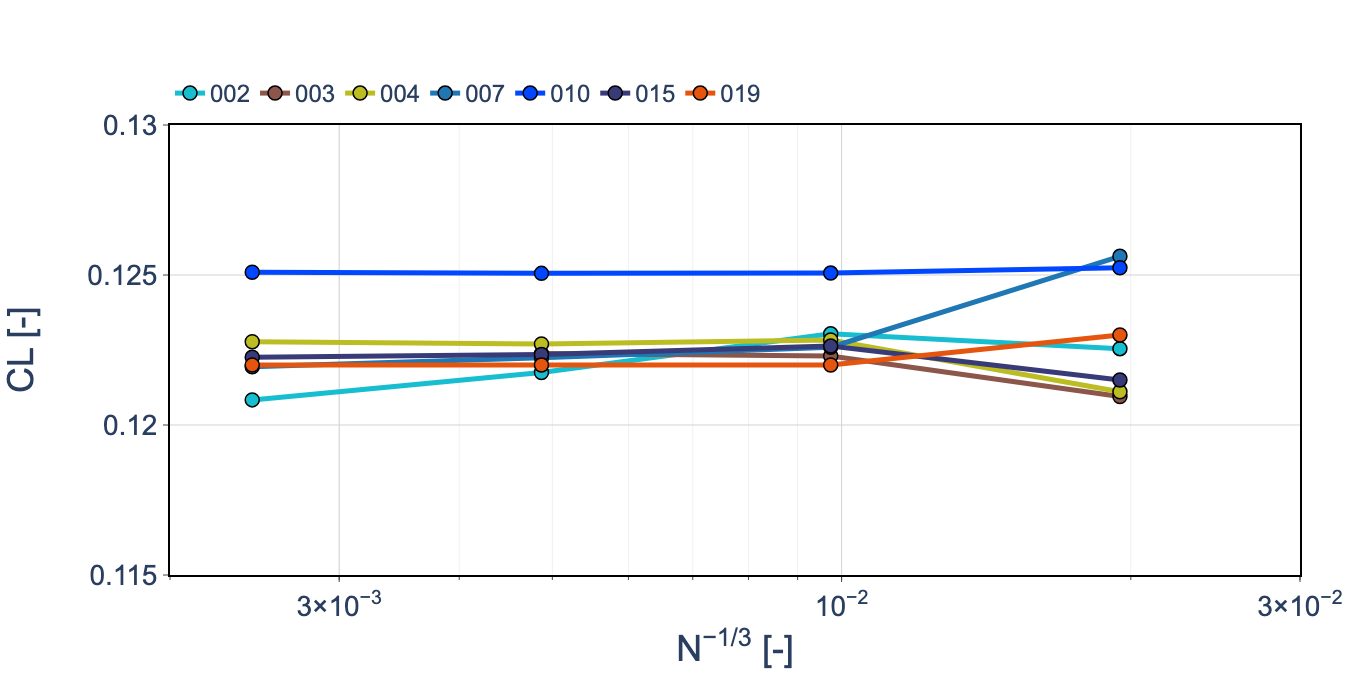
\includegraphics[width=0.48\textwidth]{FIGURES/AERODYNAMIC/tc_oneram6_cl_vs_n_1mm.png}
\hfill
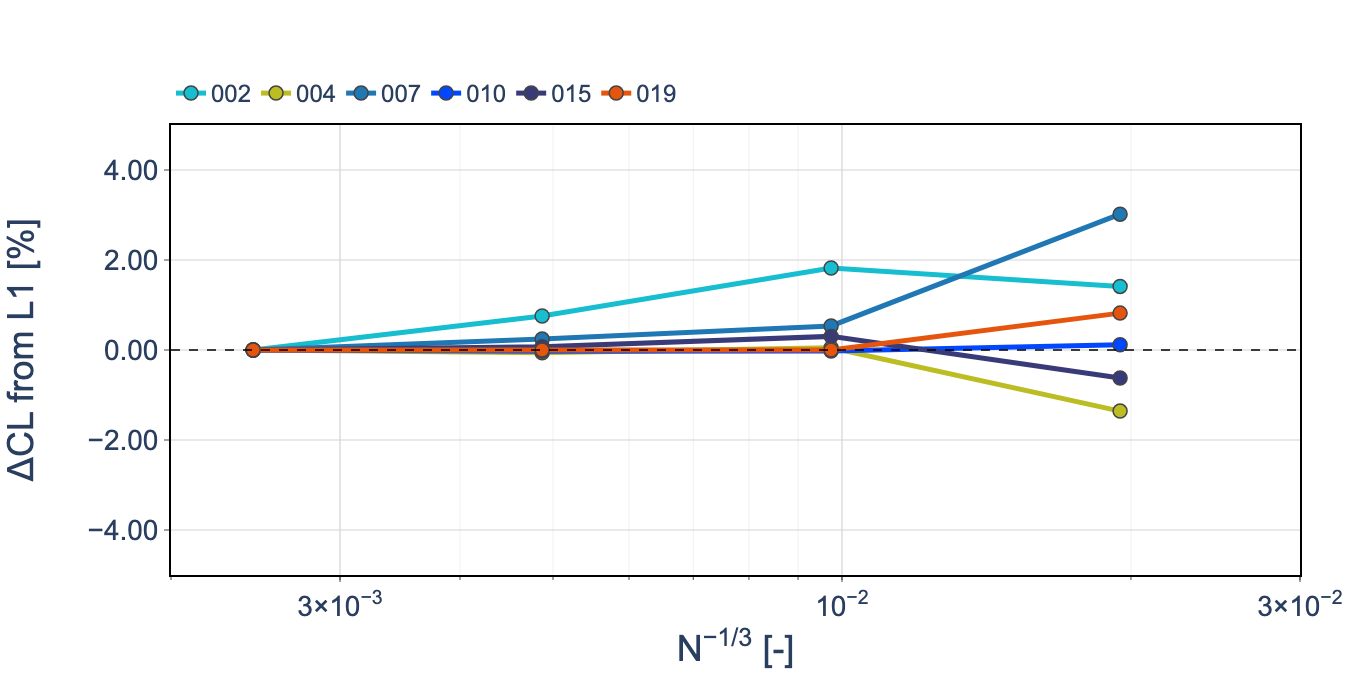
\includegraphics[width=0.48\textwidth]{FIGURES/AERODYNAMIC/tc_oneram6_cl_vs_n_1mm_relative_to_l1.png}
\par}

\vspace{0.15cm}

\begin{block}{\scriptsize Assessment}
\begin{itemize}
    \item At L1, the median lift coefficient is $C_L=0.12213$, with an IQR of $6.89\times10^{-4}$ ($0.56\%$).
    \item Coarse-grid deviations generally remain within a few percent of the corresponding L1 predictions.
    \item The code-to-code spread in $C_L$ remains small across the grid levels.
\end{itemize}
\end{block}

\end{frame}


% ============================================================
% ONERA M6 -- Aerodynamic Grid Convergence: CD
% ============================================================

\begin{frame}{\small ONERA M6 -- Drag Coefficient Grid Convergence}
\scriptsize

{\centering
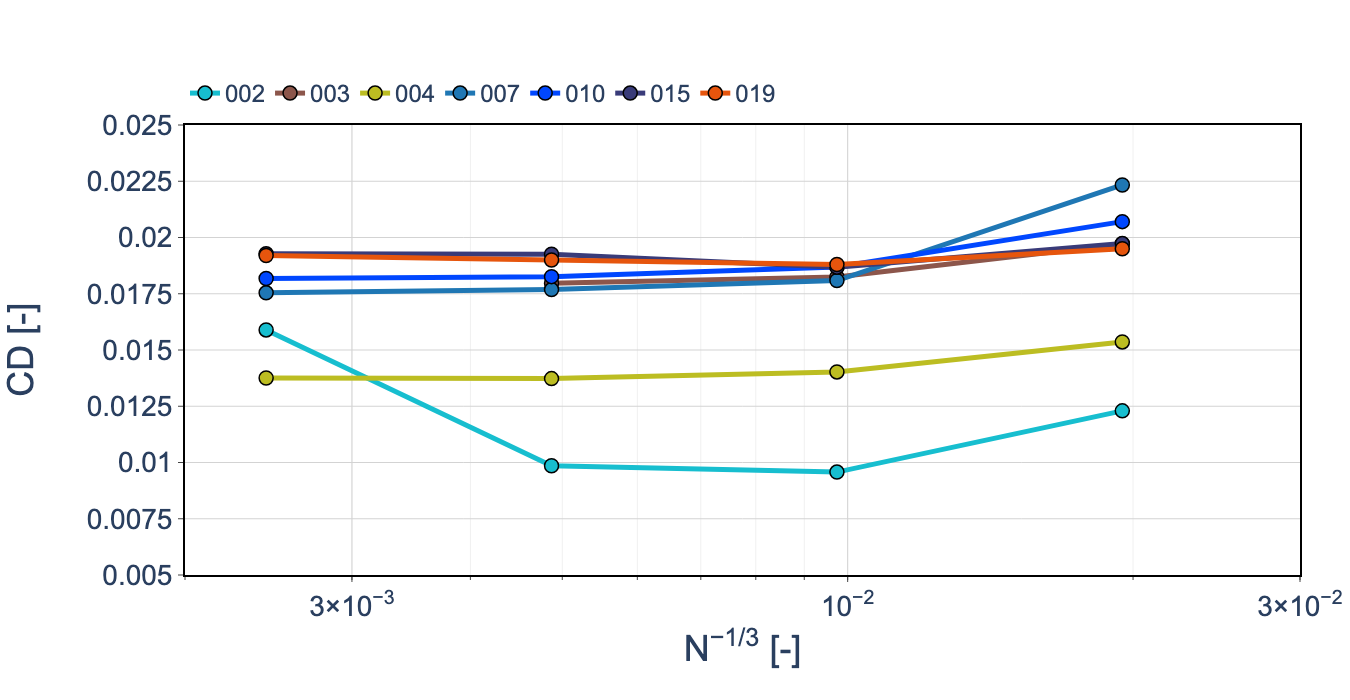
\includegraphics[width=0.48\textwidth]{FIGURES/AERODYNAMIC/tc_oneram6_cd_vs_n_1mm.png}
\hfill
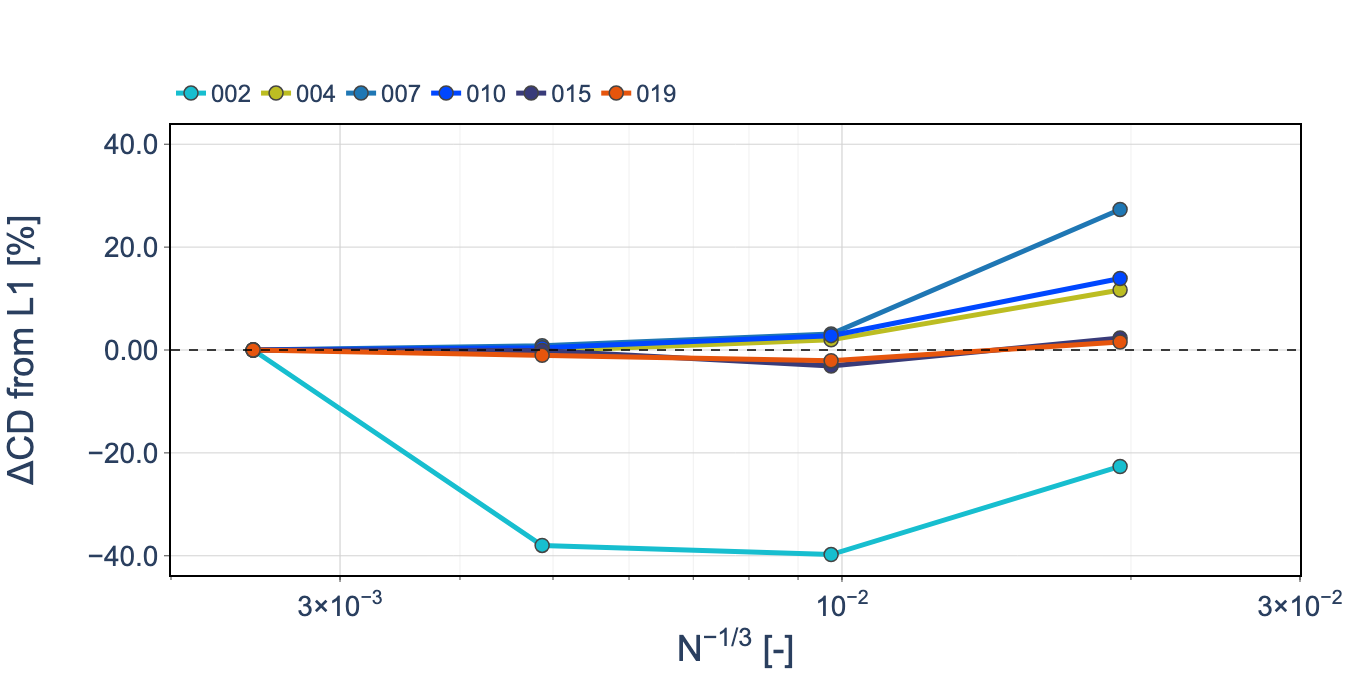
\includegraphics[width=0.48\textwidth]{FIGURES/AERODYNAMIC/tc_oneram6_cd_vs_n_1mm_relative_to_l1.png}
\par}

\vspace{0.15cm}

\begin{block}{\scriptsize Assessment}
\begin{itemize}
    \item At L1, the median drag coefficient is $C_D=0.01786$ (178.6 drag counts), with an IQR of $2.64\times10^{-3}$ (26.4 drag counts, $14.8\%$).
    \item $C_D$ exhibits considerably larger code-to-code variability than $C_L$.
    \item Several submissions show non-monotonic sensitivity to spatial grid refinement.
    \item Relative deviations from the corresponding L1 predictions reach approximately $40\%$ for selected submissions.
    \item Flow-convergence difficulties were reported for some submissions and may contribute to the observed grid sensitivity and variability in $C_D$.
\end{itemize}
\end{block}

\end{frame}


% ============================================================
% ONERA M6 -- Aerodynamic Grid Convergence: CM
% ============================================================

\begin{frame}{\small ONERA M6 -- Pitching Moment Grid Convergence}
\scriptsize

{\centering
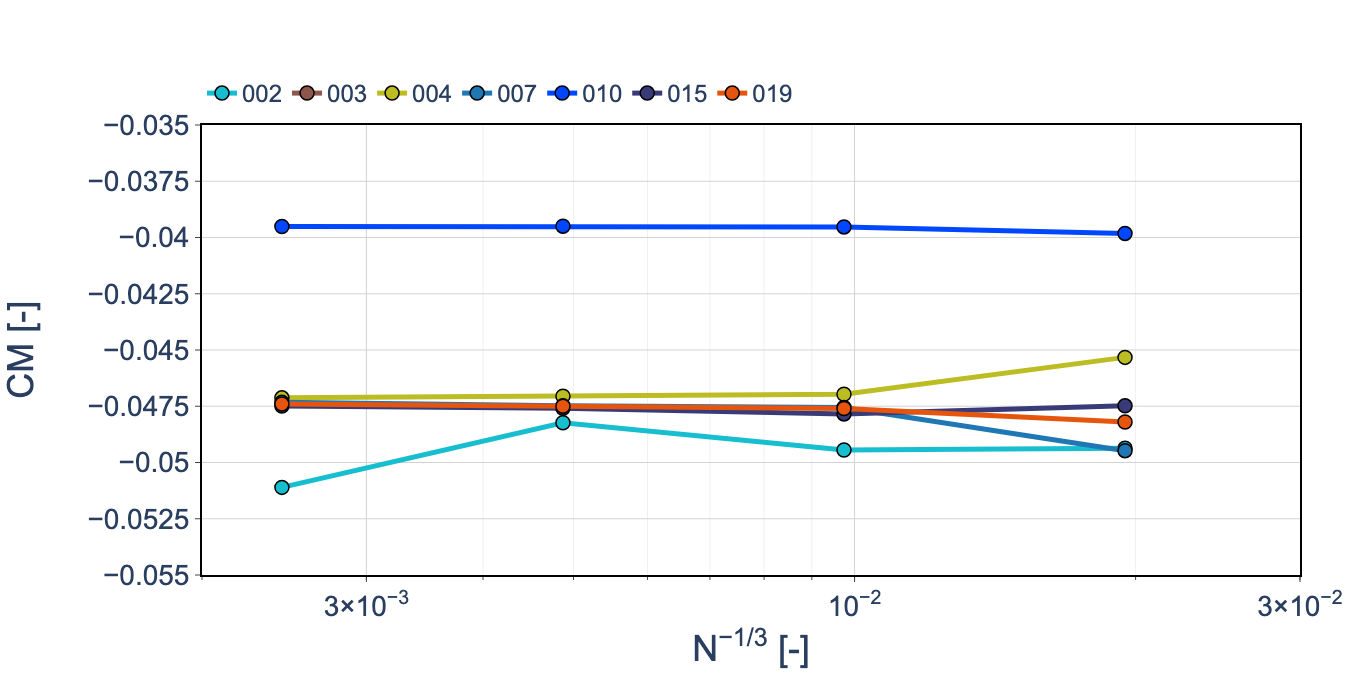
\includegraphics[width=0.48\textwidth]{FIGURES/AERODYNAMIC/tc_oneram6_cmy_vs_n_1mm.png}
\hfill
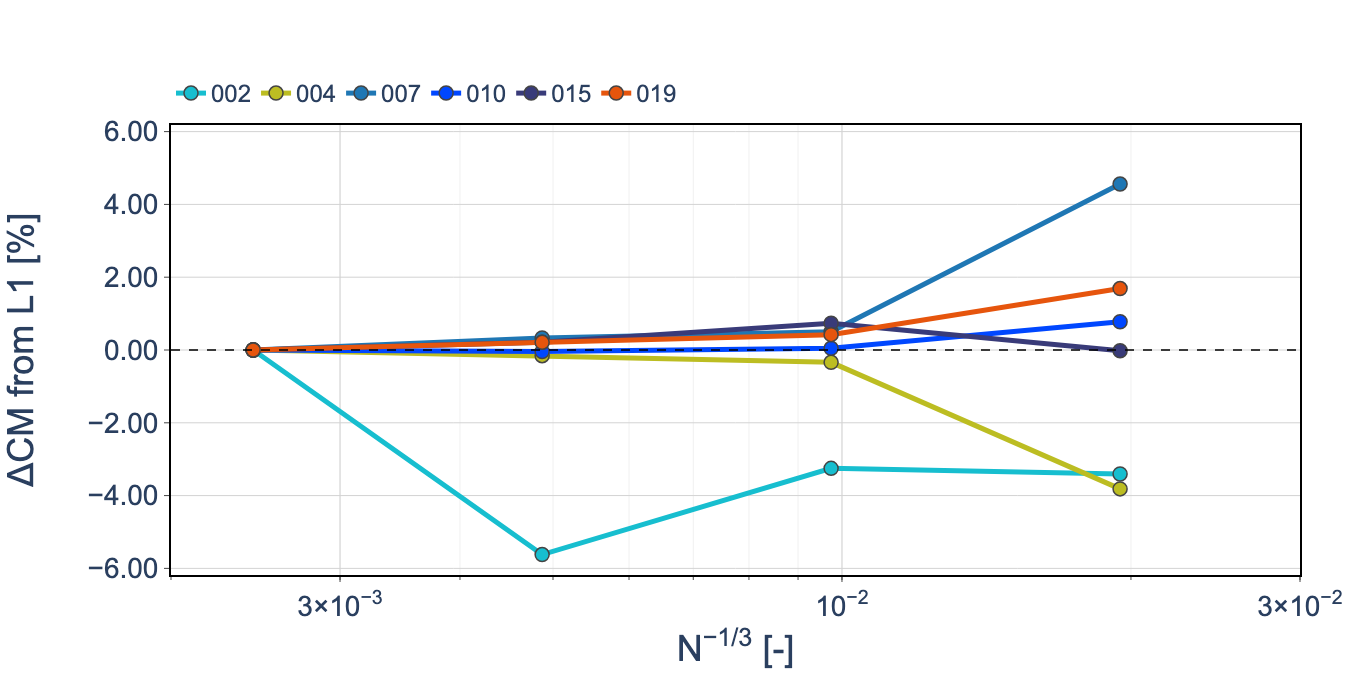
\includegraphics[width=0.48\textwidth]{FIGURES/AERODYNAMIC/tc_oneram6_cmy_vs_n_1mm_relative_to_l1.png}
\par}

\vspace{0.15cm}

\begin{block}{\scriptsize Assessment}
\begin{itemize}
    \item At L1, the median pitching-moment coefficient is $C_M=-0.04736$, with an IQR of $2.93\times10^{-4}$ ($0.62\%$).
    \item Most submissions exhibit limited sensitivity to spatial grid refinement.
\end{itemize}
\end{block}

\end{frame}


% ============================================================
% ONERA M6 -- Surface Pressure Distribution
% ============================================================

\begin{frame}{\small ONERA M6 -- Surface Pressure Distribution (L1)}
\scriptsize

% ------------------------------------------------------------
% Middle slice
% ------------------------------------------------------------
\only<1>{
\centering
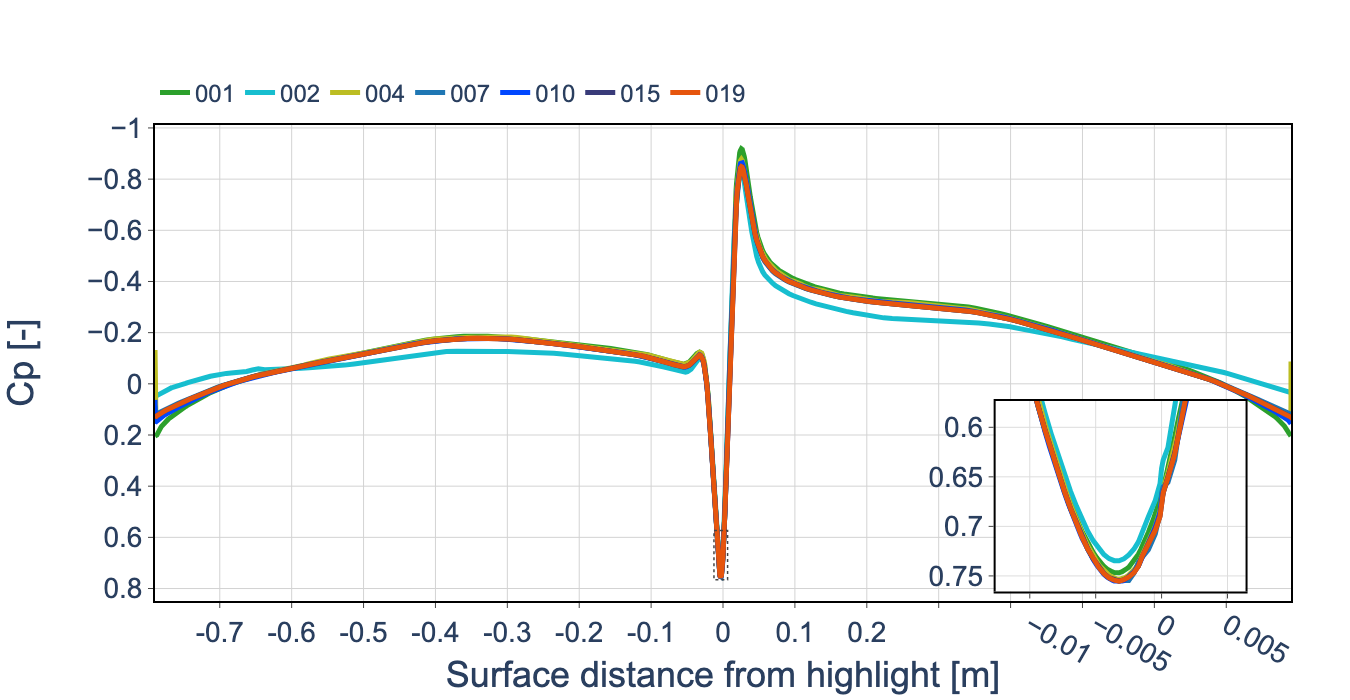
\includegraphics[width=0.62\textwidth]{FIGURES/AERODYNAMIC/tc_oneram6_L1_cp_vs_s_slice_0p75_roughness_1mm.png}

\vspace{0.05cm}

$y=0.75$ m
}

% ------------------------------------------------------------
% Inboard and outboard slices
% ------------------------------------------------------------
\only<2>{
\begin{columns}[T,onlytextwidth]

\begin{column}{0.50\textwidth}
    \centering
    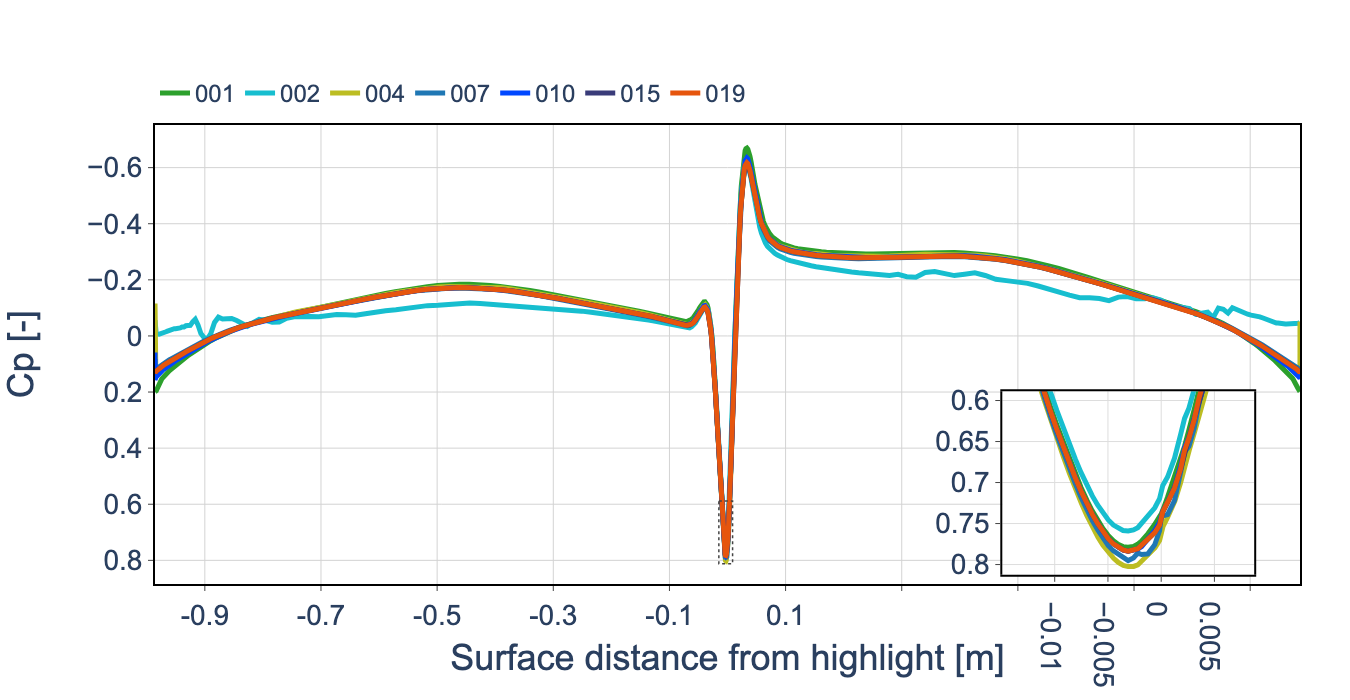
\includegraphics[width=0.94\textwidth]{FIGURES/AERODYNAMIC/tc_oneram6_L1_cp_vs_s_slice_0p1_roughness_1mm.png}

    \vspace{0.05cm}

    $y=0.10$ m
\end{column}

\begin{column}{0.50\textwidth}
    \centering
    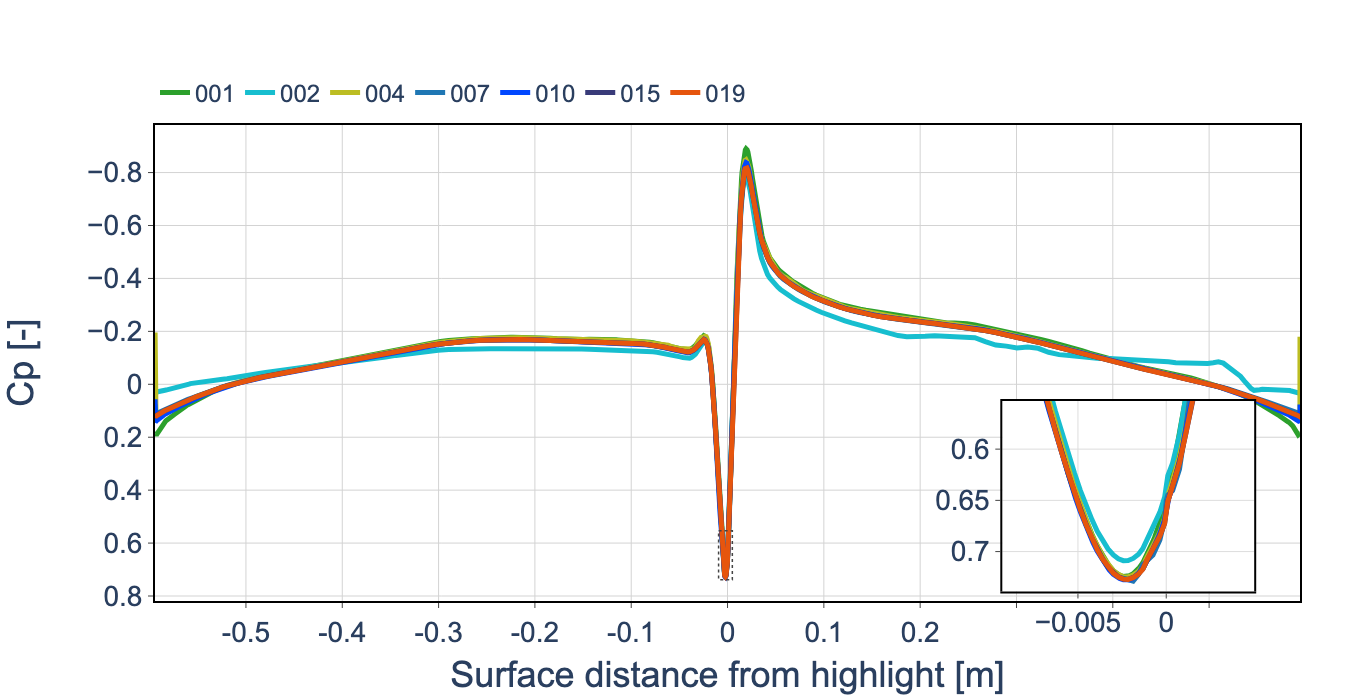
\includegraphics[width=0.94\textwidth]{FIGURES/AERODYNAMIC/tc_oneram6_L1_cp_vs_s_slice_1p4_roughness_1mm.png}

    \vspace{0.05cm}

    $y=1.40$ m
\end{column}

\end{columns}
}

\vspace{0.10cm}

\begin{block}{\scriptsize Assessment}
\begin{itemize}
    \item The submitted $C_p$ distributions are generally closely clustered across all three spanwise locations.
    \item The characteristic pressure variations associated with the leading-edge and suction-side peak are consistently captured by the participants.
    \item<2-> Overall agreement remains similar from the inboard to the outboard spanwise stations.
\end{itemize}
\end{block}

\end{frame}


% ============================================================
% ONERA M6 -- Aerodynamic Assessment Summary
% ============================================================

\begin{frame}{\small ONERA M6 -- Aerodynamic Assessment Summary}
\scriptsize

\begin{block}{\scriptsize Grid Convergence}
\begin{itemize}
    \item \textbf{$C_L$:} very weak grid sensitivity, with closely clustered predictions across the grid hierarchy.
    \item \textbf{$C_D$:} substantially greater grid sensitivity and code-to-code variability, including non-monotonic behavior for selected submissions.
    \item \textbf{$C_M$:} limited within-code grid sensitivity for most submissions.
\end{itemize}
\end{block}

\vspace{0.15cm}

\begin{block}{\scriptsize Code-to-Code Variability at L1}
\begin{center}
\begin{tabular}{lccc}
\toprule
 & \textbf{Median} & \textbf{IQR} & \textbf{Relative IQR} \\
\midrule
$C_L$ & $0.12213$  & $6.89\times10^{-4}$ & $0.56\%$ \\
$C_D$ & $0.01786$  & $2.64\times10^{-3}$ & $14.8\%$ \\
$C_M$ & $-0.04736$ & $2.93\times10^{-4}$ & $0.62\%$ \\
\bottomrule
\end{tabular}
\end{center}
\end{block}

\vspace{0.15cm}

\begin{alertblock}{\scriptsize Aerodynamic Takeaway}
The lift and pitching-moment predictions exhibit weak grid sensitivity and relatively tight code-to-code agreement for most submissions. In contrast, drag remains considerably more sensitive to both numerical implementation and spatial resolution. The $C_p$ distributions are nevertheless consistently reproduced across the three spanwise stations.
\end{alertblock}

\end{frame}


% ============================================================
% ============================================================
% END -- ONERA M6 AERODYNAMIC GRID CONVERGENCE
% ============================================================
% ============================================================
% ============================================================
% ============================================================
% NACA0012 -- DROPLET IMPINGEMENT
% ============================================================
% ============================================================

\section[Imp.]{\textbf{Droplet Impingement}}


% ============================================================
% ONERA M6 -- Collection Efficiency Profiles
% ============================================================

\begin{frame}[shrink]{\small ONERA M6 -- Collection Efficiency (15 Bins, L1)}
\scriptsize

% ------------------------------------------------------------
% Middle slice
% ------------------------------------------------------------
\only<1>{
\centering
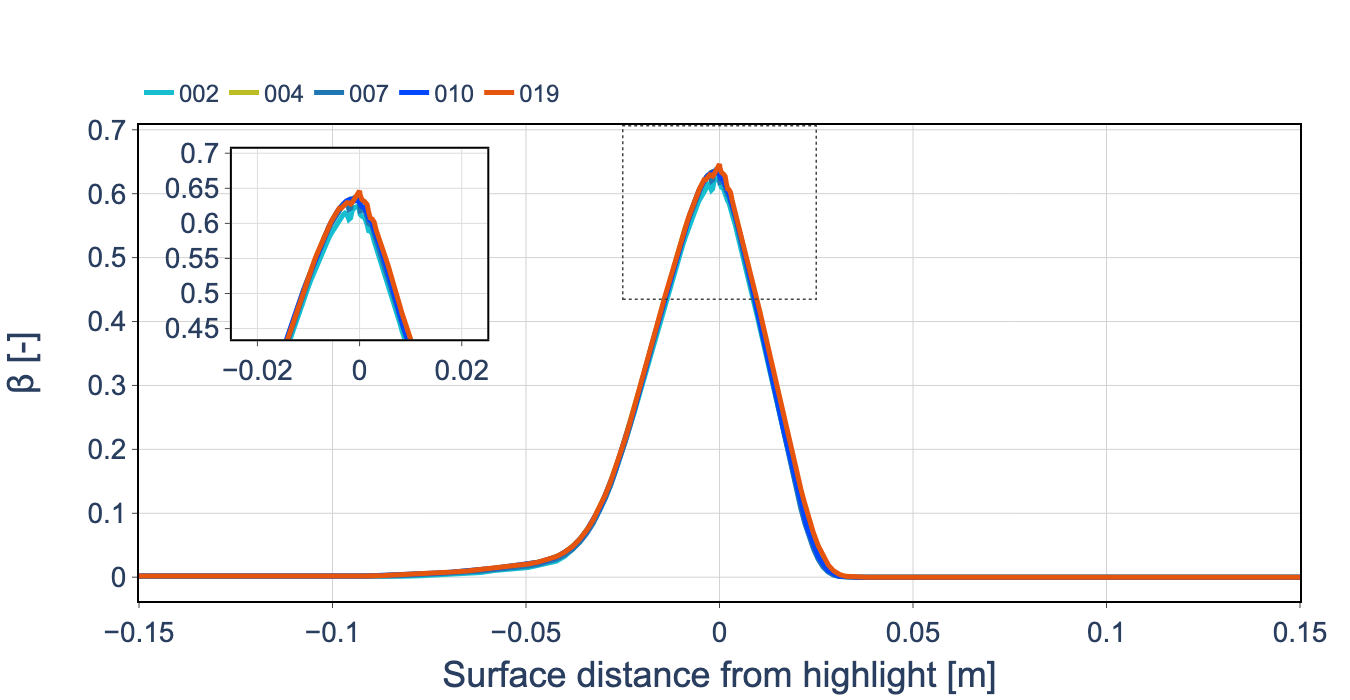
\includegraphics[width=0.62\textwidth]{FIGURES/IMPINGEMENT/tc_oneram6_L1_beta_bins15_vs_s_slice_0p75_roughness_1mm.png}

\vspace{0.05cm}

\textbf{$y=0.75$ m}
}

% ------------------------------------------------------------
% Inboard and outboard slices
% ------------------------------------------------------------
\only<2>{
\begin{columns}[T,onlytextwidth]

\begin{column}{0.49\textwidth}
    \centering
    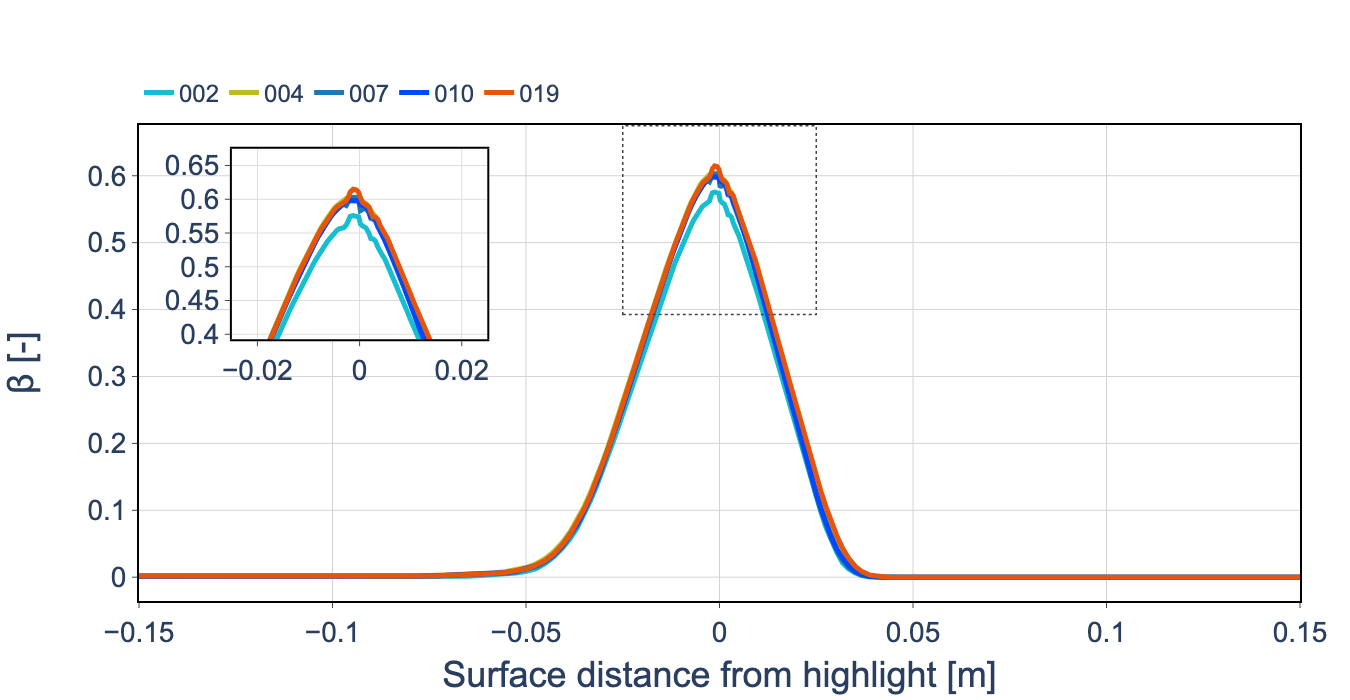
\includegraphics[width=0.96\textwidth]{FIGURES/IMPINGEMENT/tc_oneram6_L1_beta_bins15_vs_s_slice_0p1_roughness_1mm.png}

    \vspace{0.05cm}

    \textbf{$y=0.10$ m}
\end{column}

\begin{column}{0.49\textwidth}
    \centering
    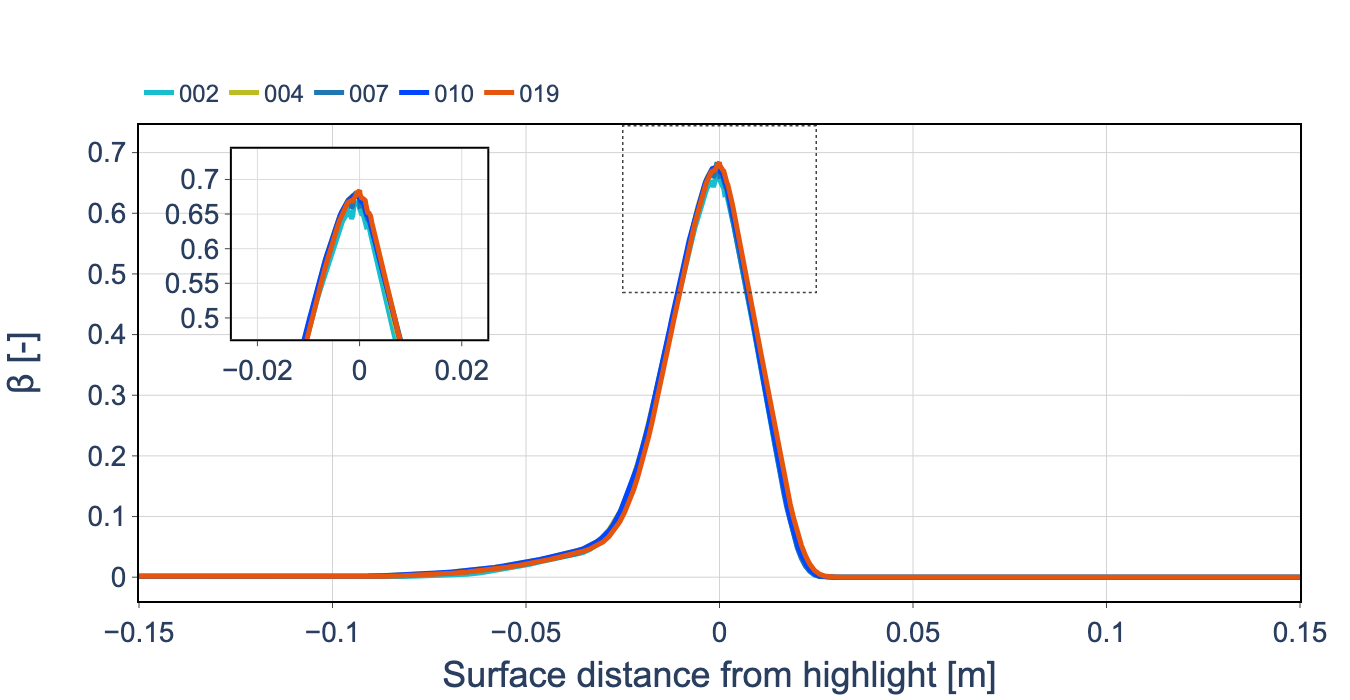
\includegraphics[width=0.96\textwidth]{FIGURES/IMPINGEMENT/tc_oneram6_L1_beta_bins15_vs_s_slice_1p4_roughness_1mm.png}

    \vspace{0.05cm}

    \textbf{$y=1.40$ m}
\end{column}

\end{columns}
}

\vspace{0.10cm}

\begin{block}{\scriptsize Assessment}
\begin{itemize}
    \item Good code-to-code agreement is observed in the collection-efficiency distribution at the representative middle spanwise station ($y=0.75$ m).
    \item The peak magnitude and location are closely clustered across submissions.
    \item<2-> Similar agreement is observed at the inboard and outboard stations.
    \item<2-> Small oscillations near the peak are likely associated with the surface discretization in the highly curved leading-edge region.
\end{itemize}
\end{block}

\end{frame}


% ============================================================
% ONERA M6 -- Water Mass Grid Convergence
% ============================================================

\begin{frame}{\small ONERA M6 -- Water Mass Grid Convergence (15 Bins)}
\scriptsize

{\centering
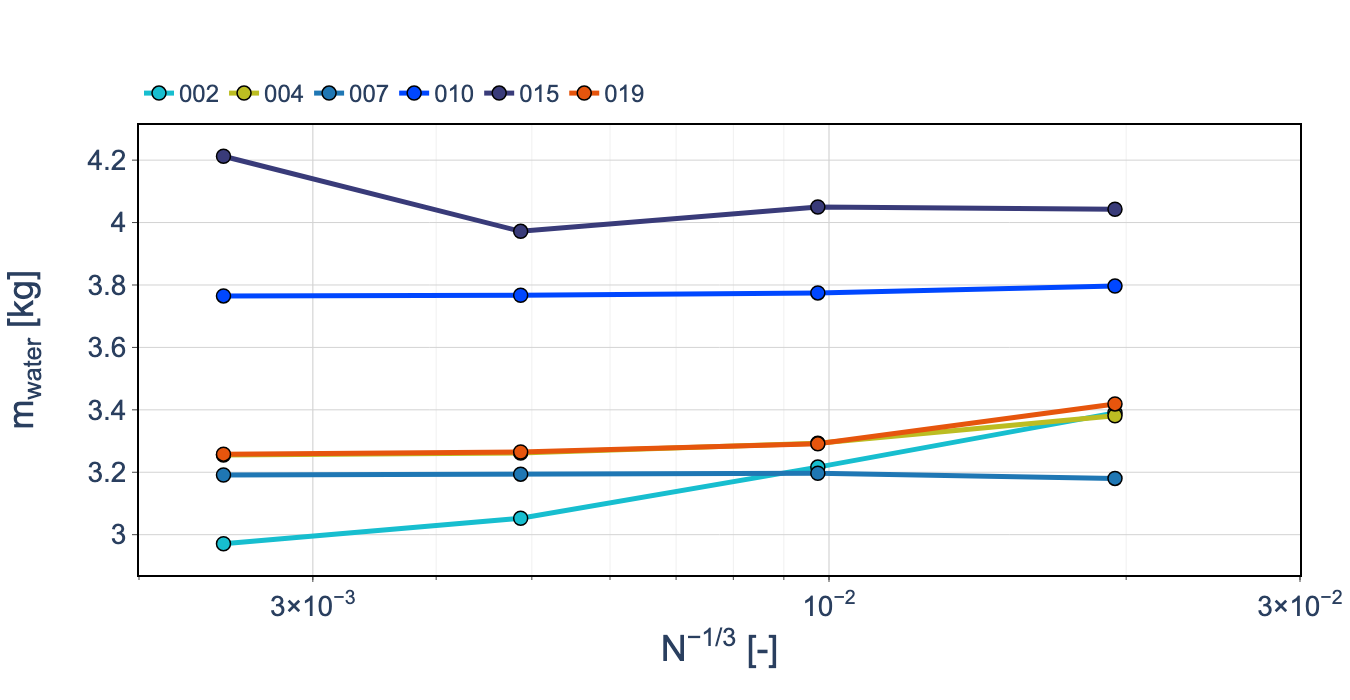
\includegraphics[width=0.48\textwidth]{FIGURES/IMPINGEMENT/tc_oneram6_water_mass_vs_n_1mm_bins15_all_grid_levels.png}
\hfill
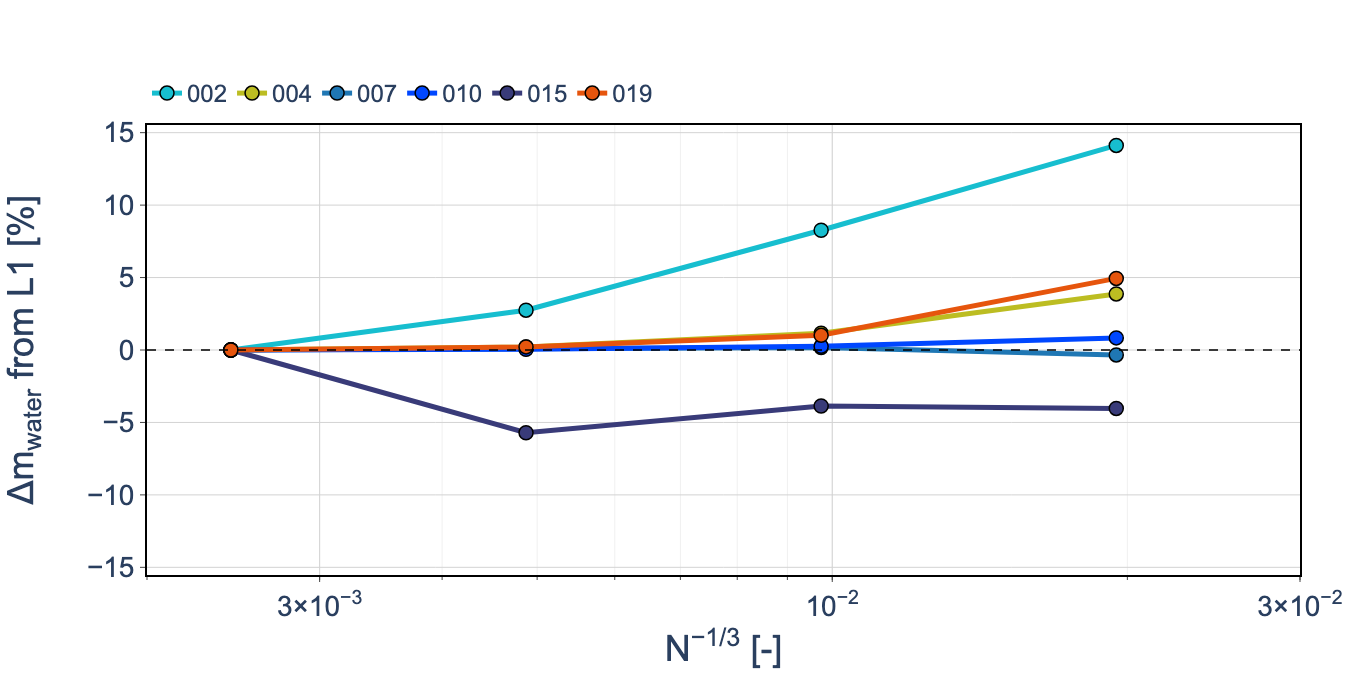
\includegraphics[width=0.48\textwidth]{FIGURES/IMPINGEMENT/tc_oneram6_water_mass_vs_n_1mm_bins15_all_grid_levels_relative_to_l1.png}
\par}

\vspace{0.15cm}

\begin{block}{\scriptsize Assessment}
\begin{itemize}
    \item For the 15-bin distribution, the L1 median water mass is $3.257~\mathrm{kg}$, with an IQR of $0.431~\mathrm{kg}$ ($13.2\%$).
    \item Most submissions exhibit limited sensitivity to spatial grid refinement, with changes generally remaining within approximately $5\%$ of their corresponding L1 predictions.
\end{itemize}
\end{block}

\end{frame}

% ============================================================
% ONERA M6 -- Droplet Distribution Sensitivity
% ============================================================

\begin{frame}{\small ONERA M6 -- Droplet Distribution Sensitivity (L1)}
\scriptsize

\begin{columns}[T,onlytextwidth]

\begin{column}{0.50\textwidth}
    \centering
    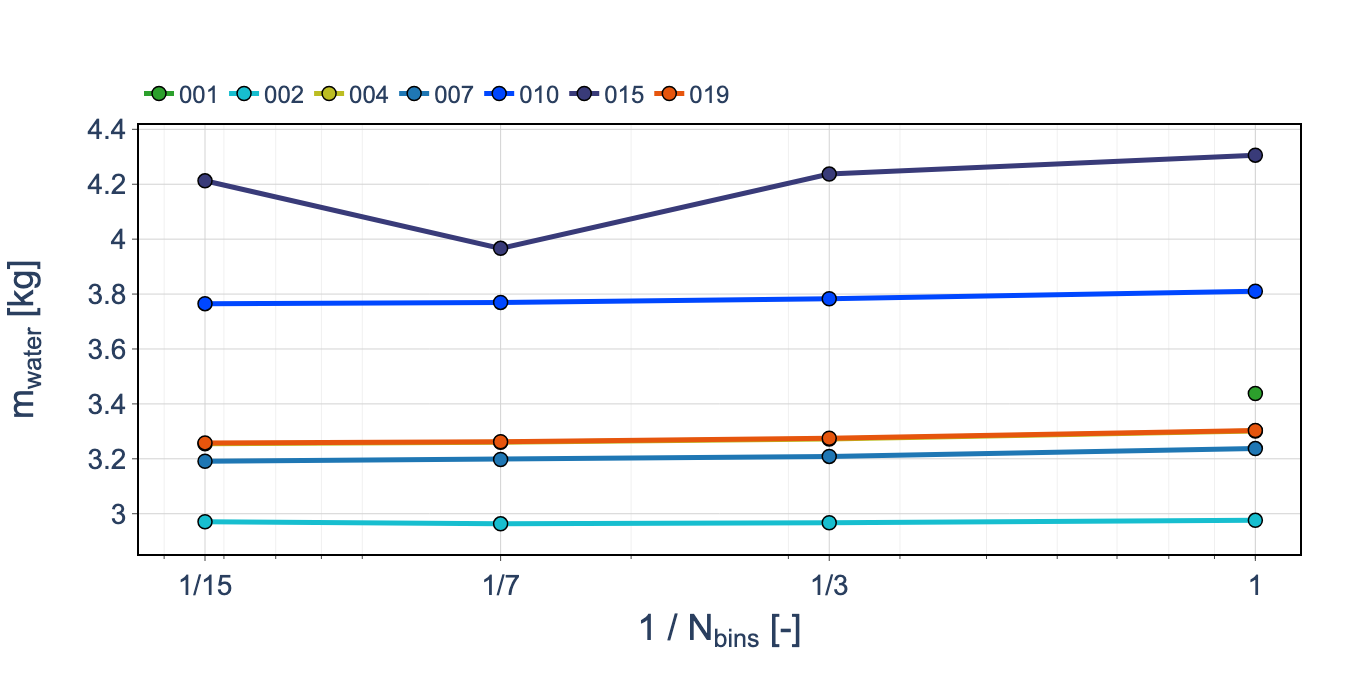
\includegraphics[width=0.96\textwidth]{FIGURES/IMPINGEMENT/tc_oneram6_water_mass_vs_n_1mm_l1_vs_inverse_bins.png}
\end{column}

\begin{column}{0.50\textwidth}
    \centering
    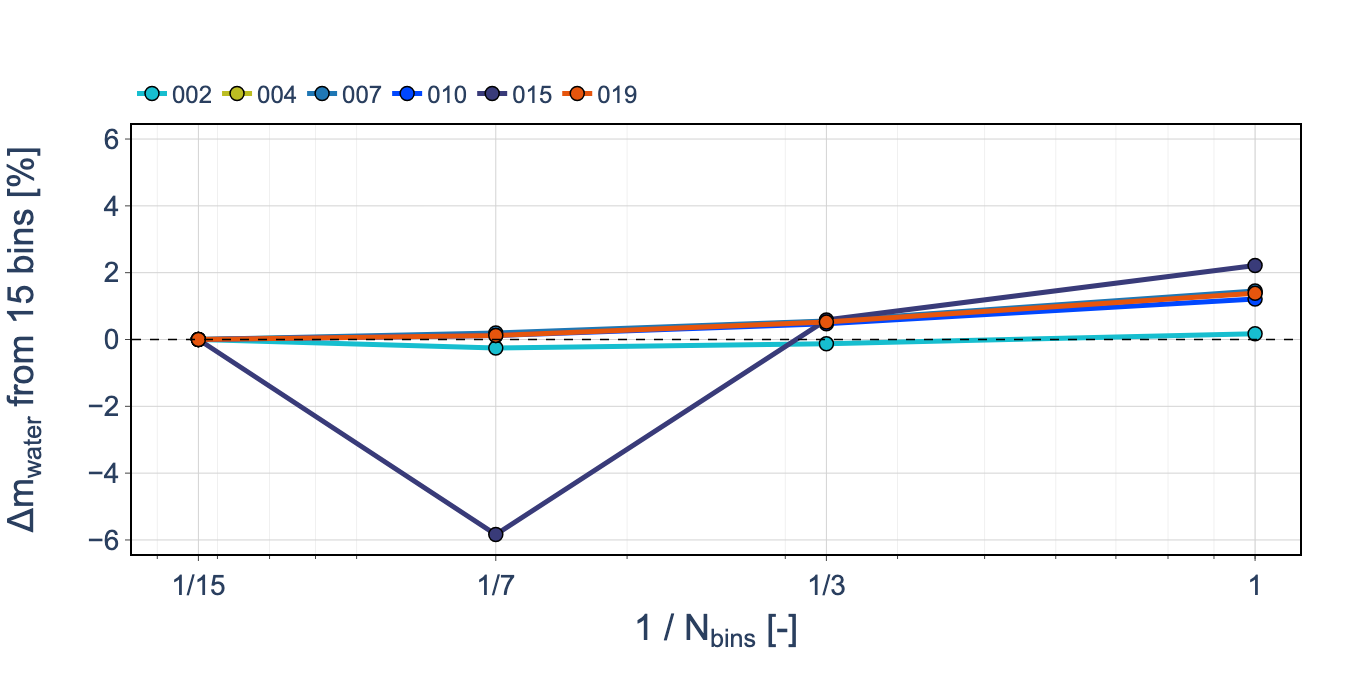
\includegraphics[width=0.96\textwidth]{FIGURES/IMPINGEMENT/tc_oneram6_water_mass_vs_n_1mm_l1_vs_inverse_bins_relative_to_bins15.png}
\end{column}

\end{columns}

\vspace{0.10cm}

\begin{block}{\scriptsize Assessment}
\begin{itemize}
    \item All the distributions produce very similar impinged water masses for most submissions.
    \item Relative differences remain within approximately $2\%$ for most submissions and distributions, with one isolated 7-bin deviation of approximately $6\%$.
    \item The narrow droplet-size range ($6.16$--$33.84~\mu$m around an MVD of $20~\mu$m) contributes to the weak distribution sensitivity.
\end{itemize}
\end{block}

\end{frame}

% ============================================================
% ONERA M6 -- Water-Mass Variability by Droplet Diameter
% ============================================================

\begin{frame}{\small ONERA M6 -- Water-Mass Variability by Droplet Diameter}
\scriptsize

\begin{columns}[c,onlytextwidth]

\begin{column}{0.50\textwidth}
    \centering
    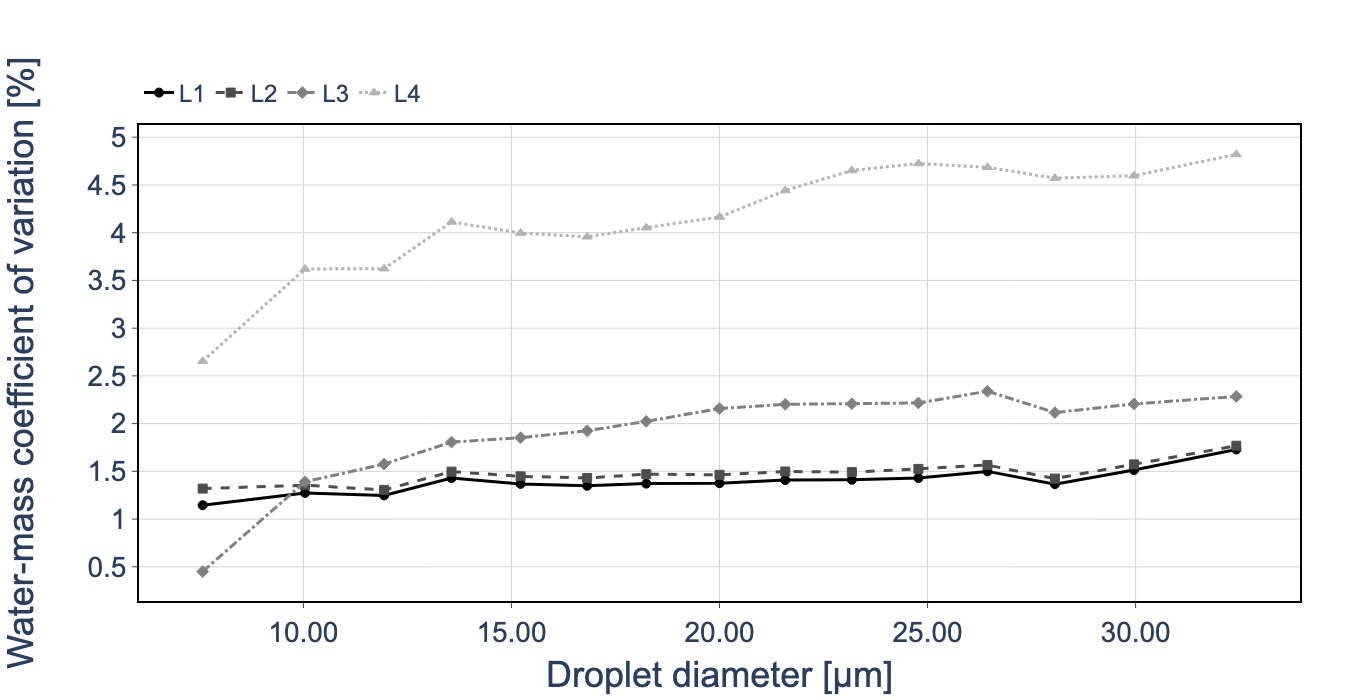
\includegraphics[width=\textwidth]{FIGURES/IMPINGEMENT/tc_oneram6_water_mass_coefficient_of_variation_vs_droplet_diameter_bins15_all_grid_levels.png}
\end{column}

\begin{column}{0.50\textwidth}
    \centering
    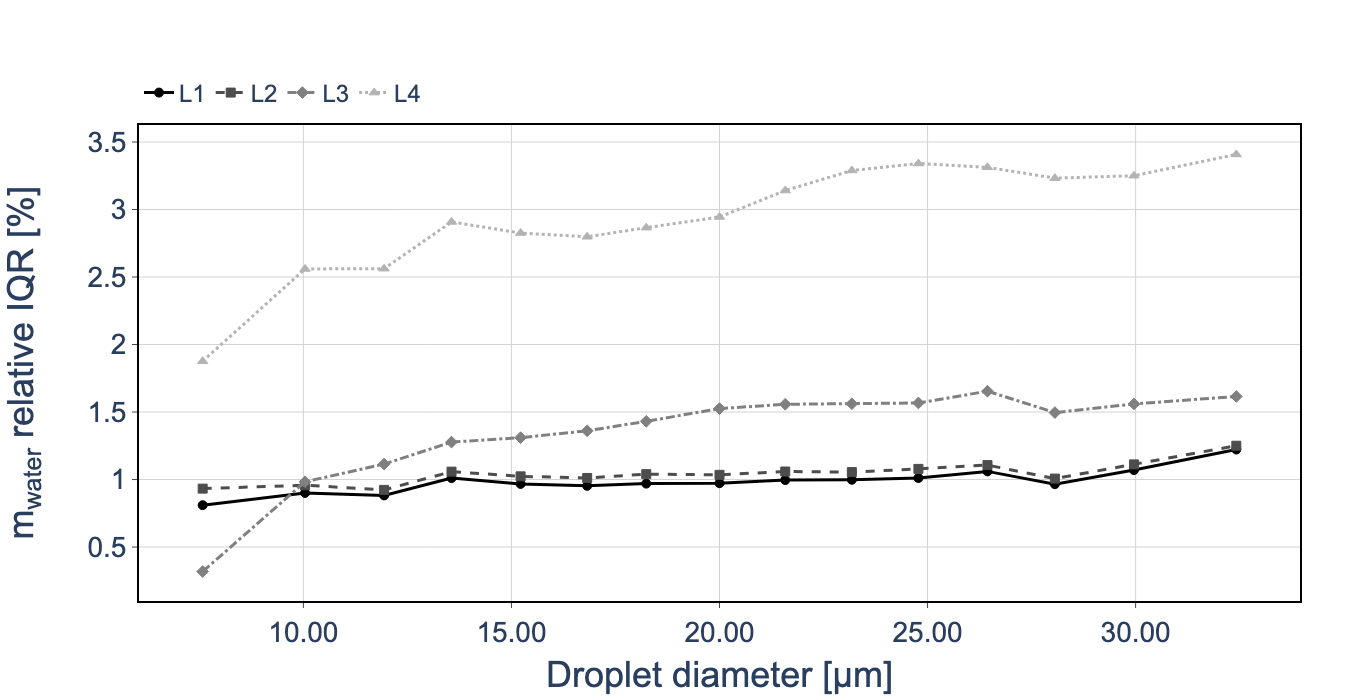
\includegraphics[width=\textwidth]{FIGURES/IMPINGEMENT/tc_oneram6_water_mass_relative_iqr_vs_droplet_diameter_bins15_all_grid_levels.png}
\end{column}

\end{columns}

\vspace{0.15cm}

\begin{block}{\scriptsize Assessment}
\begin{itemize}
    \item On the fine L1 and L2 grids, the code-to-code variability remains low across the entire droplet-diameter range, with relative IQR values generally around $1\%$.
    \item Variability increases on the coarser L3 and L4 grids, indicating a stronger grid-resolution effect than droplet-size dependence.
    \item No pronounced dependence on droplet diameter is observed over the relatively narrow $6.16$--$33.84~\mu$m range, centered around an MVD of $20~\mu$m.
    \item This relatively narrow droplet-size distribution also helps explain the weak sensitivity of the integrated impinged water mass to the number of bins.
\end{itemize}
\end{block}

\end{frame}

% ============================================================
% ONERA M6 -- Impingement Width Grid Convergence
% ============================================================

\begin{frame}{\small ONERA M6 -- Impingement Width Grid Convergence (15 Bins)}
\scriptsize

\begin{columns}[c,onlytextwidth]

\begin{column}{0.49\textwidth}
    \centering
    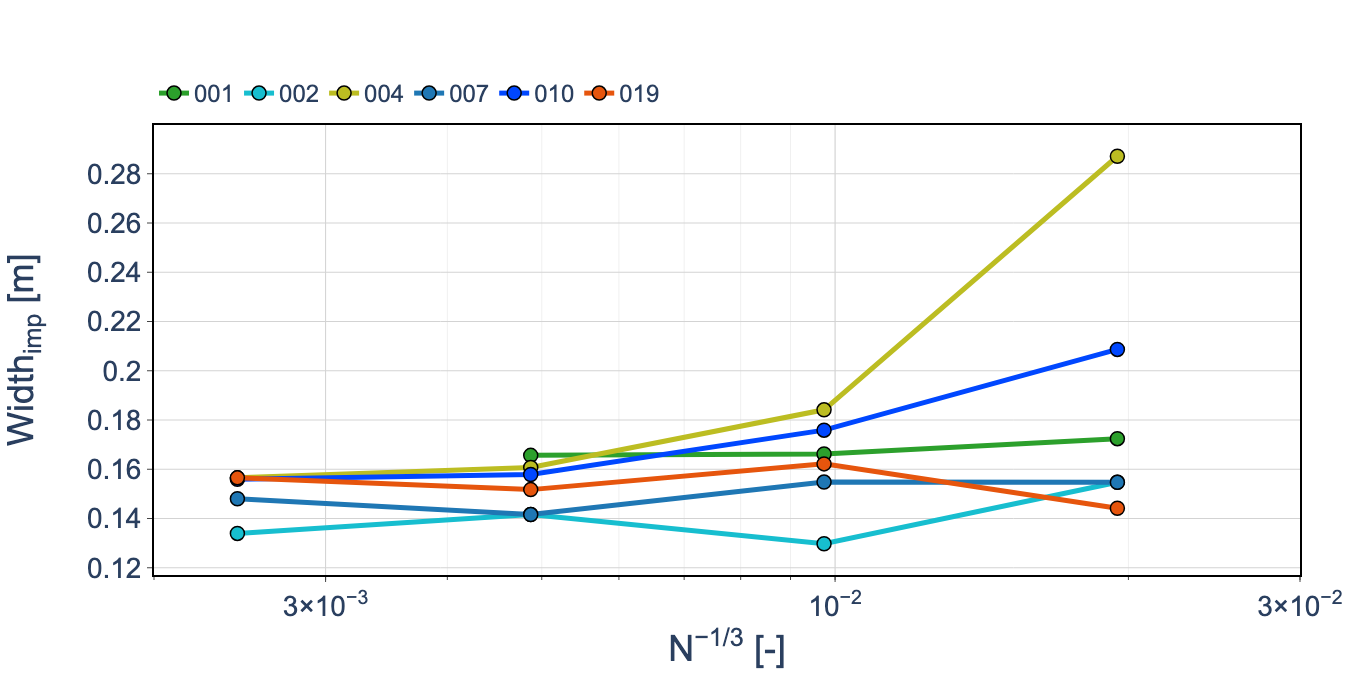
\includegraphics[width=\textwidth]{FIGURES/IMPINGEMENT/tc_oneram6_width_bins15_0_75.png}

    \vspace{-0.10cm}
    \textbf{$y=0.75$ m}
\end{column}

\begin{column}{0.49\textwidth}
    \centering
    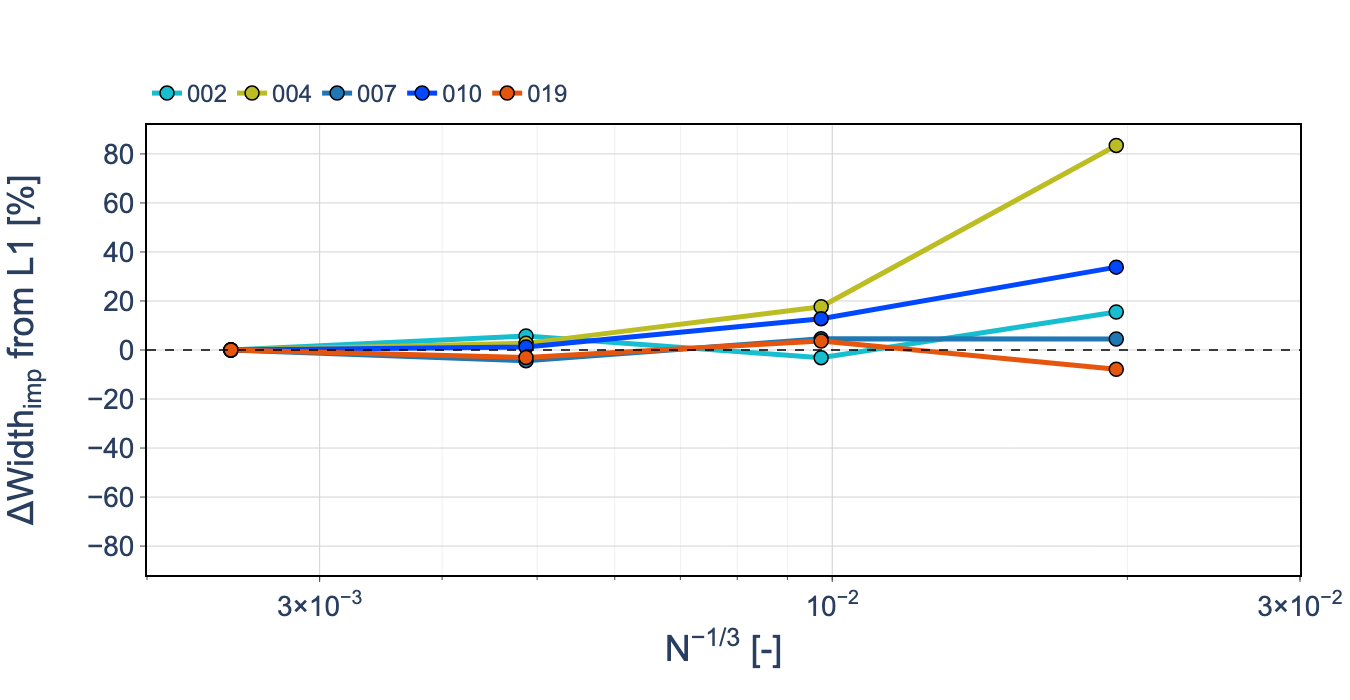
\includegraphics[width=\textwidth]{FIGURES/IMPINGEMENT/tc_oneram6_width_bins15_0_75_relative_to_l1.png}
\end{column}

\end{columns}

\vspace{0.15cm}

\begin{block}{\scriptsize Assessment}
\begin{itemize}
    \item Due to the oscillations observed near the $\beta$ peak, the peak magnitude and position are excluded from the grid-convergence assessment; the impingement width is retained as the primary profile-based metric.
    \item The impingement width is defined from the lower and upper $\beta=0.001$ threshold crossings.
    \item Most submissions show comparatively limited grid sensitivity between L1 and L2.
    \item Larger and non-monotonic deviations are observed on the coarser grids for several submissions, indicating greater sensitivity of the predicted impingement limits to spatial resolution.
\end{itemize}
\end{block}

\end{frame}

% ============================================================
% ONERA M6 -- Impingement Width Distribution Sensitivity
% ============================================================

\begin{frame}{\small ONERA M6 -- Impingement Width Distribution Sensitivity (L1)}
\scriptsize

\begin{columns}[c,onlytextwidth]

\begin{column}{0.49\textwidth}
    \centering
    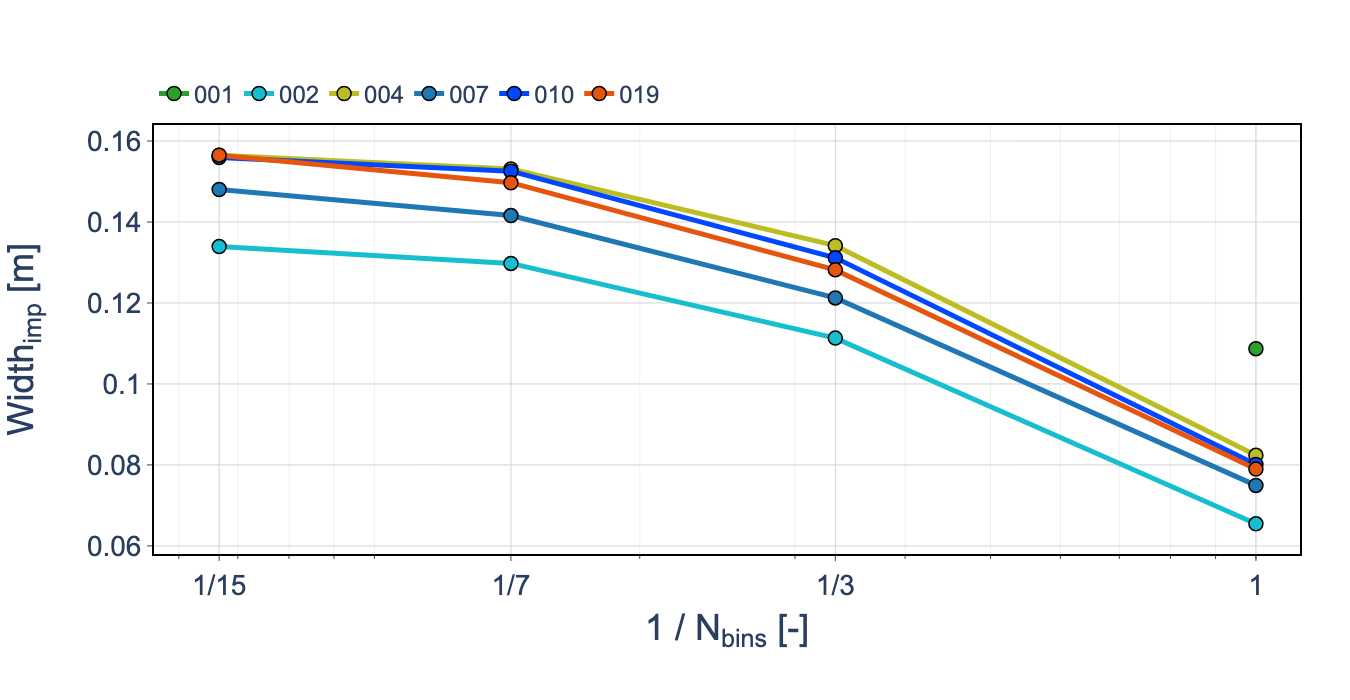
\includegraphics[width=\textwidth]{FIGURES/IMPINGEMENT/tc_oneram6_width_distribution_convergence_l1_0_75.png}

    \vspace{-0.10cm}
    \textbf{$y=0.75$ m}
\end{column}

\begin{column}{0.49\textwidth}
    \centering
    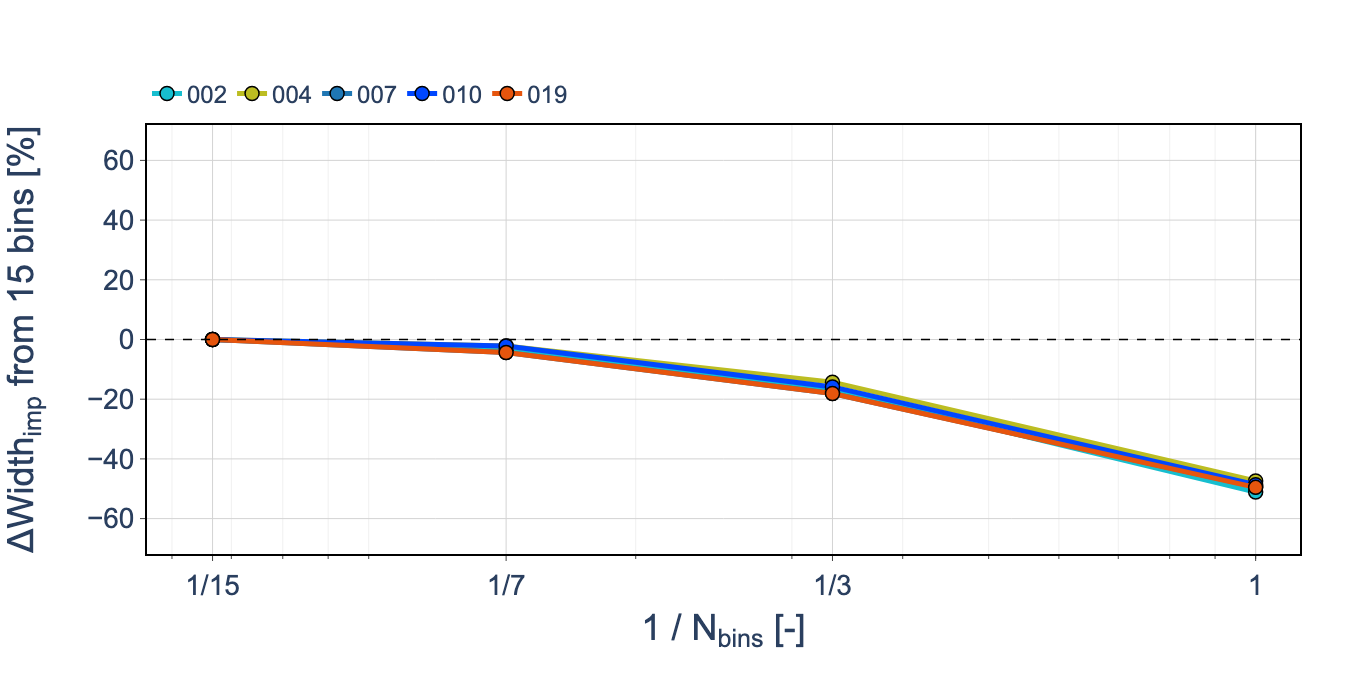
\includegraphics[width=\textwidth]{FIGURES/IMPINGEMENT/tc_oneram6_width_distribution_convergence_l1_0_75_relative_to_bins15.png}
\end{column}

\end{columns}

\vspace{0.15cm}

\begin{block}{\scriptsize Assessment}
\begin{itemize}
    \item The predicted impingement width systematically increases as the droplet distribution is refined from 1 to 15 bins.
    \item A noticeable increase remains between the 7- and 15-bin distributions, indicating that convergence with respect to droplet-distribution resolution has not yet been clearly demonstrated.
    \item In contrast, the integrated impinged water mass varies by only approximately $2\%$ between the single- and 15-bin distributions for most submissions.
    \item Droplet-distribution resolution therefore has a substantially stronger influence on the spatial extent of impingement than on the integrated collected water mass.
\end{itemize}
\end{block}

\end{frame}

% ============================================================
% ONERA M6 -- Droplet Impingement Summary
% ============================================================

\begin{frame}{\small ONERA M6 -- Droplet Impingement Summary}
\scriptsize

\begin{block}{\scriptsize Spatial Grid Convergence}
\begin{itemize}
    \item Collection-efficiency distributions show good code-to-code agreement across the three spanwise stations.
    \item Integrated water mass exhibits limited grid sensitivity for most submissions, while code-to-code differences remain larger.
    \item Impingement limits are more sensitive to spatial resolution, particularly on the coarser grids.
\end{itemize}
\end{block}

\vspace{0.15cm}

\begin{block}{\scriptsize Droplet-Size Distribution}
\begin{itemize}
    \item Integrated water mass is weakly sensitive to droplet discretization; even the single-MVD approximation remains within approximately $2\%$ of the 15-bin prediction for most submissions.
    \item In contrast, impingement width systematically increases from 1 to 15 bins, with convergence not yet clearly demonstrated at 15 bins.
    \item The relatively narrow $6.16$--$33.84~\mu$m range around the $20~\mu$m MVD contributes to the weak sensitivity of the integrated water mass.
\end{itemize}
\end{block}

\vspace{0.15cm}

\begin{alertblock}{\scriptsize Impingement Takeaway}
Integrated water mass can appear converged while the spatial impingement extent remains sensitive to both spatial and droplet-distribution resolution.
\end{alertblock}

\end{frame}

% ============================================================
% ============================================================
% NACA0012 -- CONVECTIVE HEAT TRANSFER
% ============================================================
% ============================================================

\section[HTC $\&$ Thermodynamic]{\textbf{Convective Heat Transfer}}

% ============================================================
% ONERA M6 -- Convective Heat-Transfer Distribution
% ============================================================

\begin{frame}[shrink]{\small ONERA M6 -- Convective Heat-Transfer Distribution (L1)}
\scriptsize

% ------------------------------------------------------------
% Middle slice -- 1 mm roughness
% ------------------------------------------------------------
\only<1>{
\centering
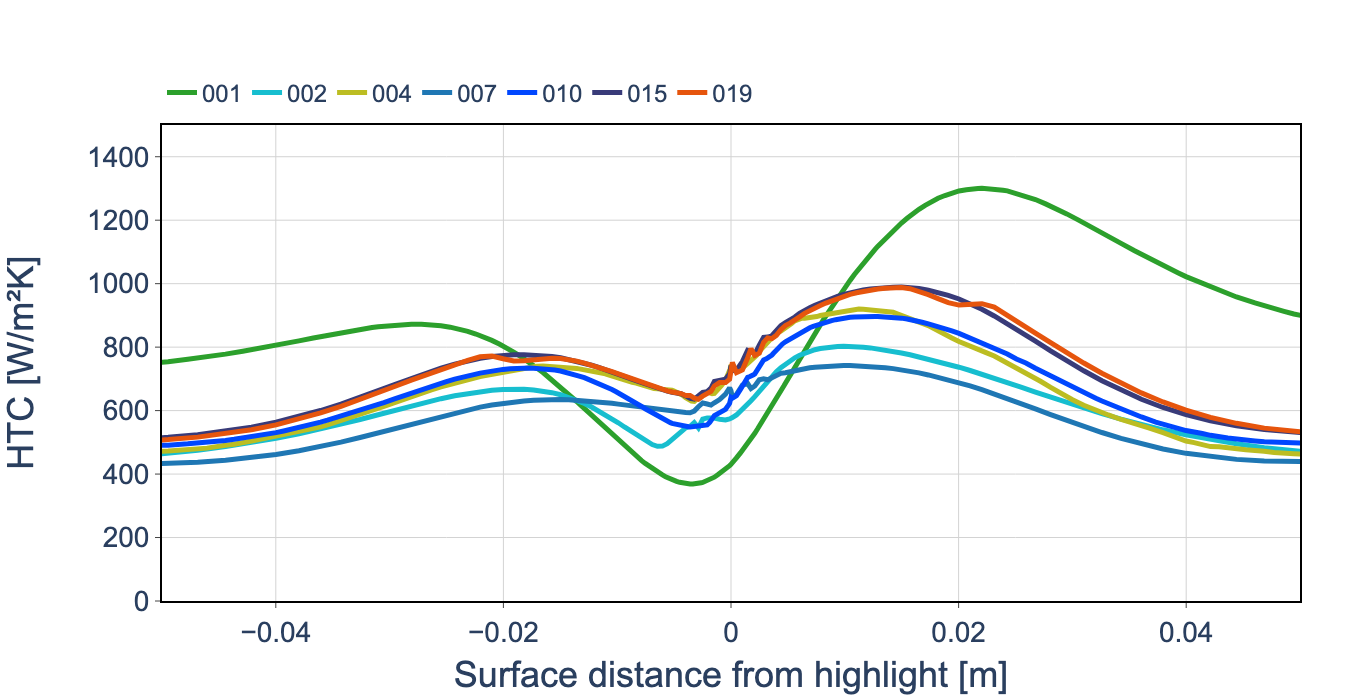
\includegraphics[width=0.5\textwidth]{FIGURES/HTC/tc_oneram6_L1_htc_vs_s_slice_0p75_roughness_1mm.png}

\vspace{0.05cm}

\textbf{$y=0.75$ m}
}

% ------------------------------------------------------------
% Inboard and outboard slices -- 1 mm roughness
% ------------------------------------------------------------
\only<2>{
\begin{columns}[T,onlytextwidth]

\begin{column}{0.50\textwidth}
    \centering
    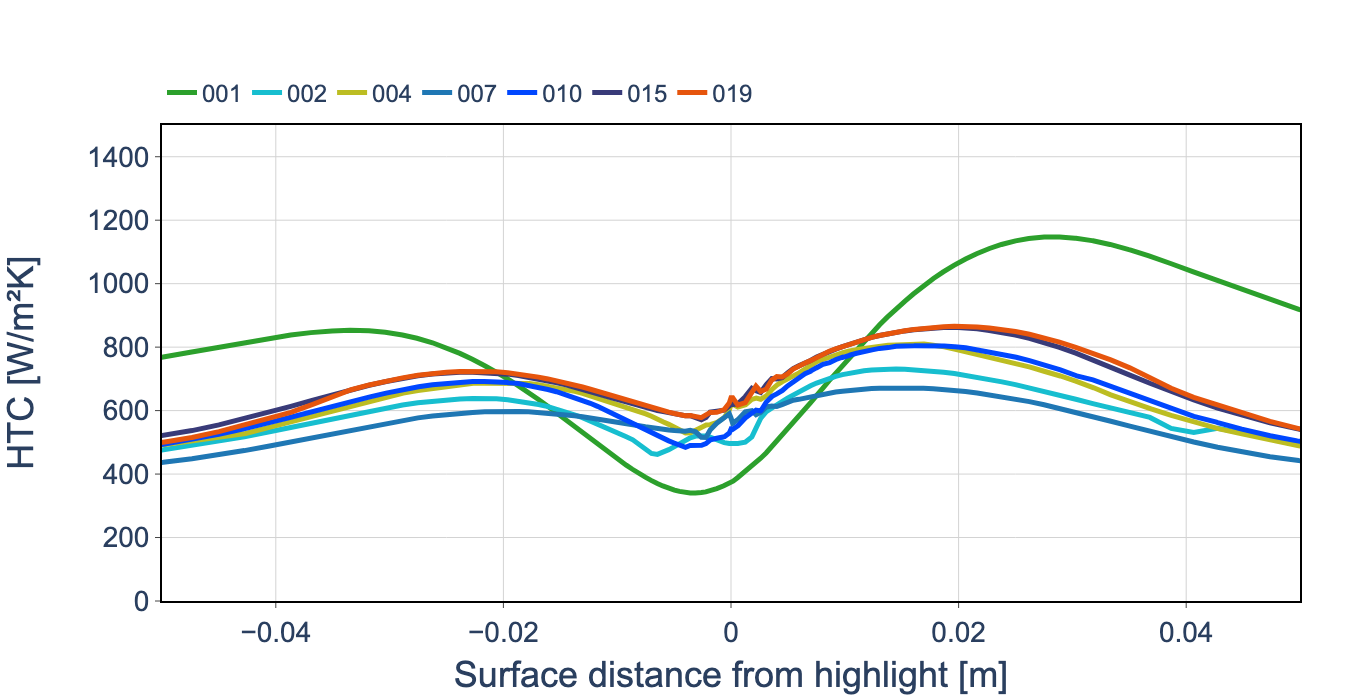
\includegraphics[width=0.94\textwidth]{FIGURES/HTC/tc_oneram6_L1_htc_vs_s_slice_0p1_roughness_1mm.png}

    \vspace{0.05cm}

    \textbf{$y=0.10$ m}
\end{column}

\begin{column}{0.50\textwidth}
    \centering
    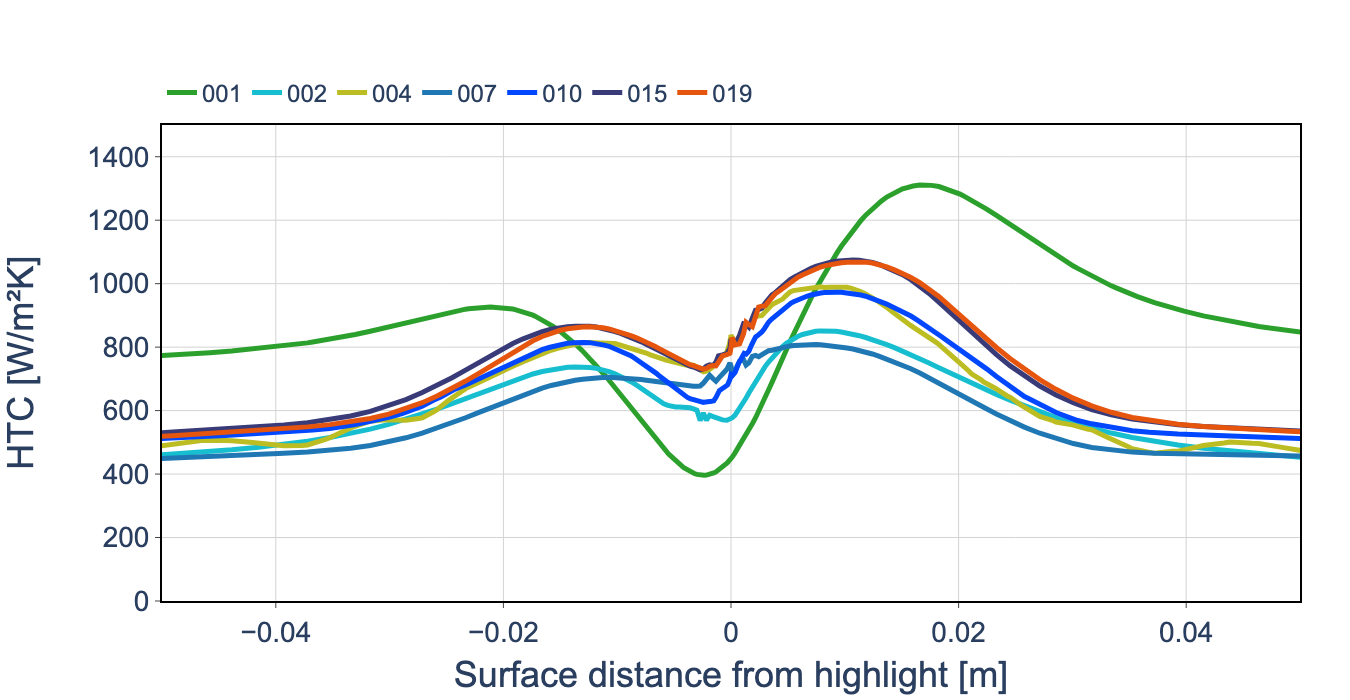
\includegraphics[width=0.94\textwidth]{FIGURES/HTC/tc_oneram6_L1_htc_vs_s_slice_1p4_roughness_1mm.png}

    \vspace{0.05cm}

    \textbf{$y=1.40$ m}
\end{column}

\end{columns}
}

% ------------------------------------------------------------
% Middle slice -- grouped by roughness
% ------------------------------------------------------------
\only<3>{
\centering
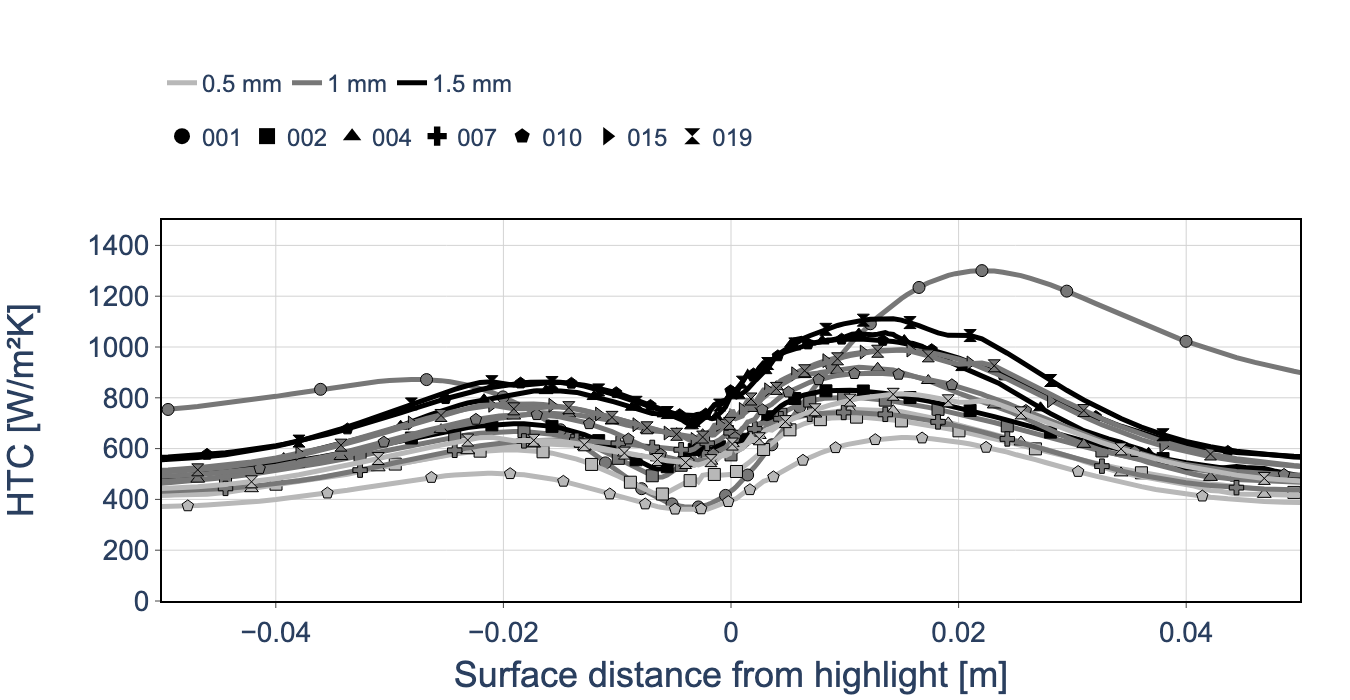
\includegraphics[width=0.62\textwidth]{FIGURES/HTC/tc_oneram6_L1_htc_vs_s_slice_0p75_all_roughness.png}

\vspace{0.05cm}

\textbf{$y=0.75$ m}
}

\vspace{0.10cm}

\begin{block}{\scriptsize Observations}
\begin{itemize}
    \item<1-> At the prescribed $1$ mm roughness, considerable code-to-code differences are observed in $HTC$, particularly near the leading edge.
    \item<2-> Similar variability is observed at the other spanwise stations, indicating that roughness alone does not explain the code-to-code scatter.
    \item<3-> Increasing roughness generally increases the predicted $HTC$, although the magnitude of the roughness effect varies between codes.
\end{itemize}
\end{block}

\end{frame}


% ============================================================
% ONERA M6 -- Participant-Level Roughness Sensitivity
% ============================================================

\begin{frame}{\small ONERA M6 -- Participant-Level HTC Roughness Sensitivity (L1)}
\scriptsize
\vspace{-0.2cm}
\centering
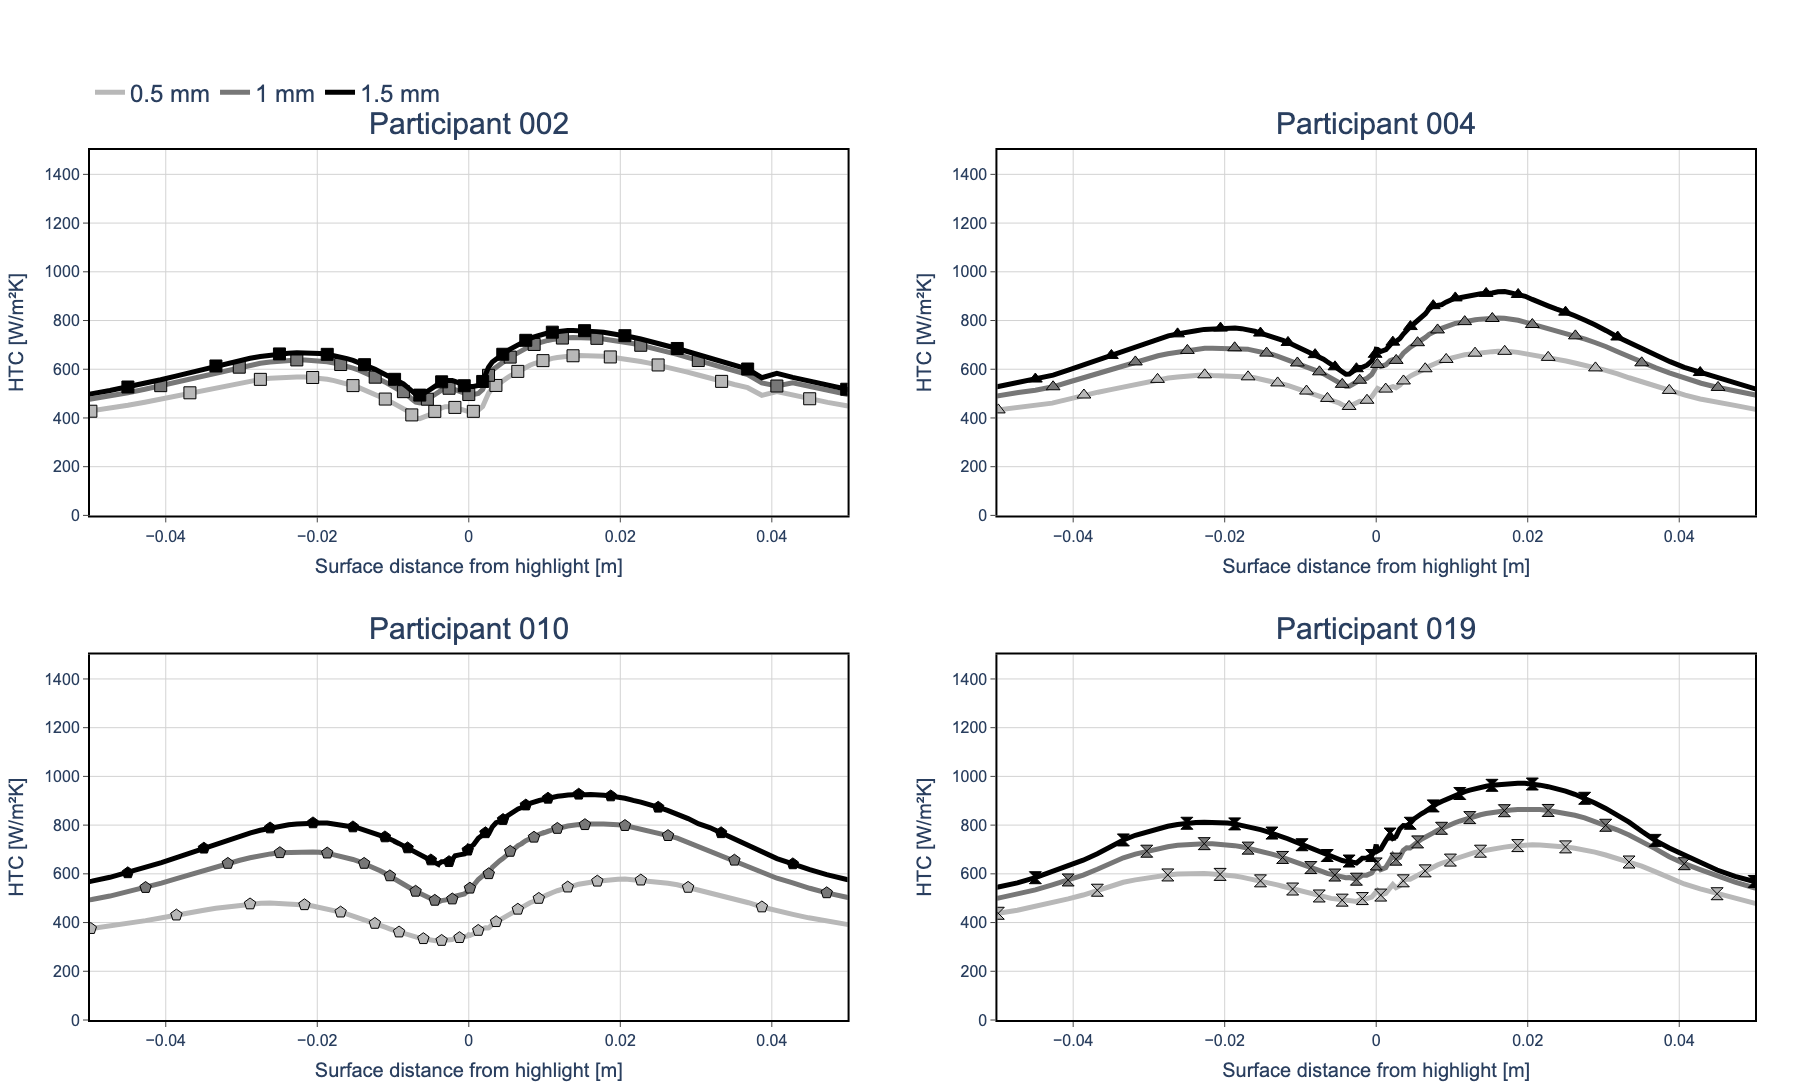
\includegraphics[width=0.8\textwidth]{FIGURES/HTC/tc_oneram6_L1_htc_vs_s_slice_0p1_all_roughness_participants.png}

\end{frame}

% ============================================================
% ============================================================
% END -- ONERA M6 CONVECTIVE HEAT TRANSFER
% ============================================================
% ============================================================

% ============================================================
% ONERA M6 -- Surface Temperature
% ============================================================

\begin{frame}{\small ONERA M6 -- Surface Temperature Distribution (L1)}
\scriptsize

% ------------------------------------------------------------
% Middle slice
% ------------------------------------------------------------
\only<1>{
\centering
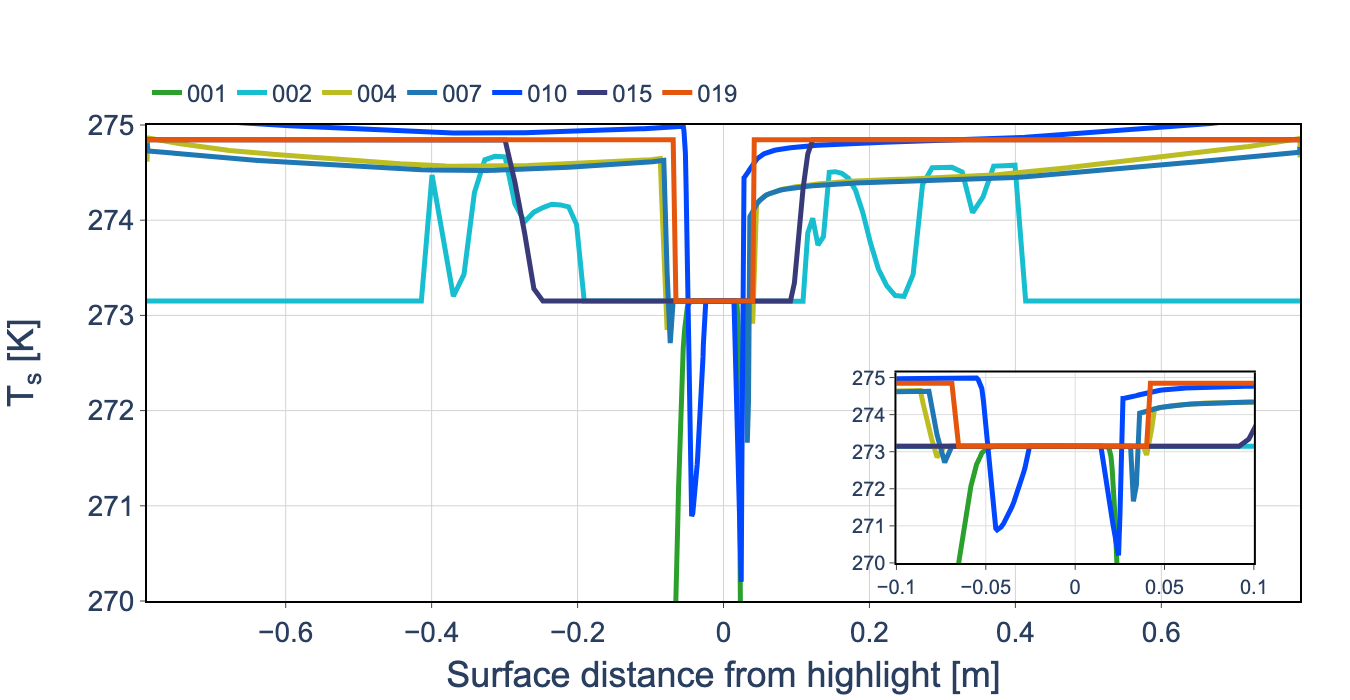
\includegraphics[width=0.5\textwidth]{FIGURES/SURF_TEMP_FF/tc_oneram6_L1_surface_temperature_vs_s_slice_0p75_roughness_1mm.png}

\vspace{0.05cm}

\textbf{$y=0.75$ m }
}

% ------------------------------------------------------------
% Inboard and outboard slices
% ------------------------------------------------------------
\only<2>{
\begin{columns}[T,onlytextwidth]

\begin{column}{0.50\textwidth}
    \centering
    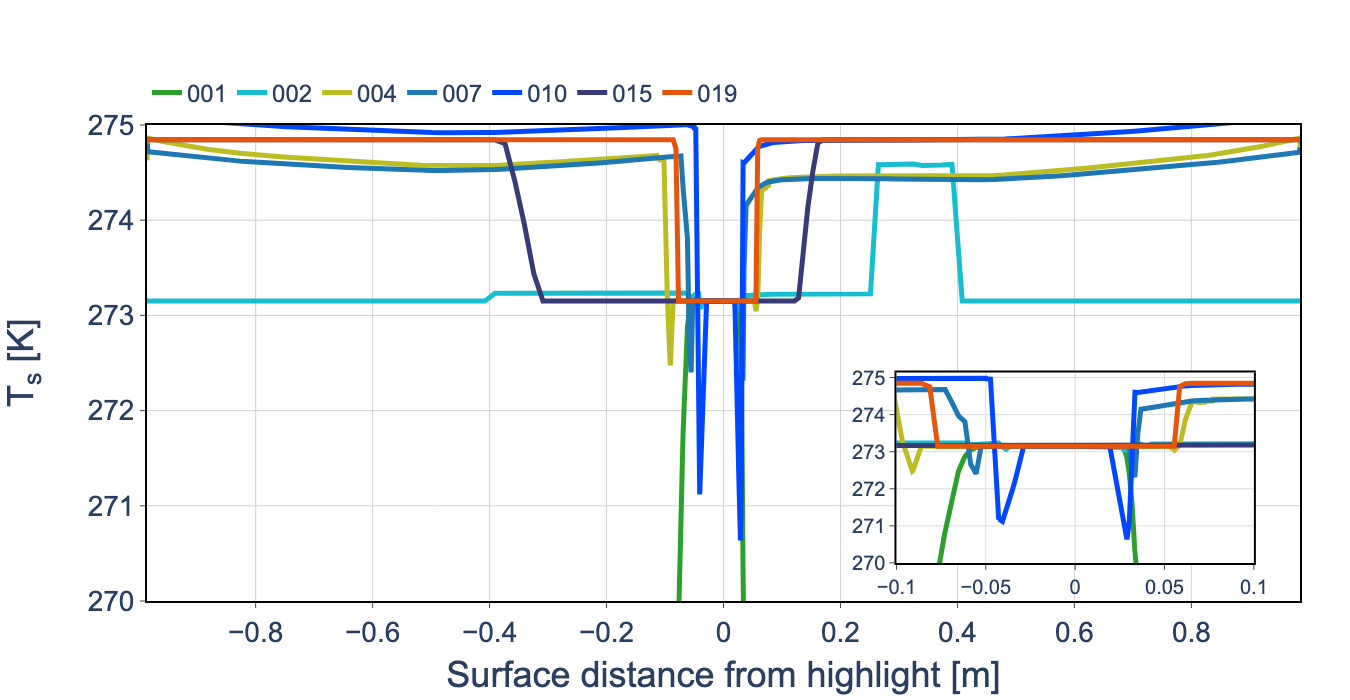
\includegraphics[width=0.94\textwidth]{FIGURES/SURF_TEMP_FF/tc_oneram6_L1_surface_temperature_vs_s_slice_0p1_roughness_1mm.png}

    \vspace{0.05cm}

    \textbf{$y=0.10$ m}
\end{column}

\begin{column}{0.50\textwidth}
    \centering
    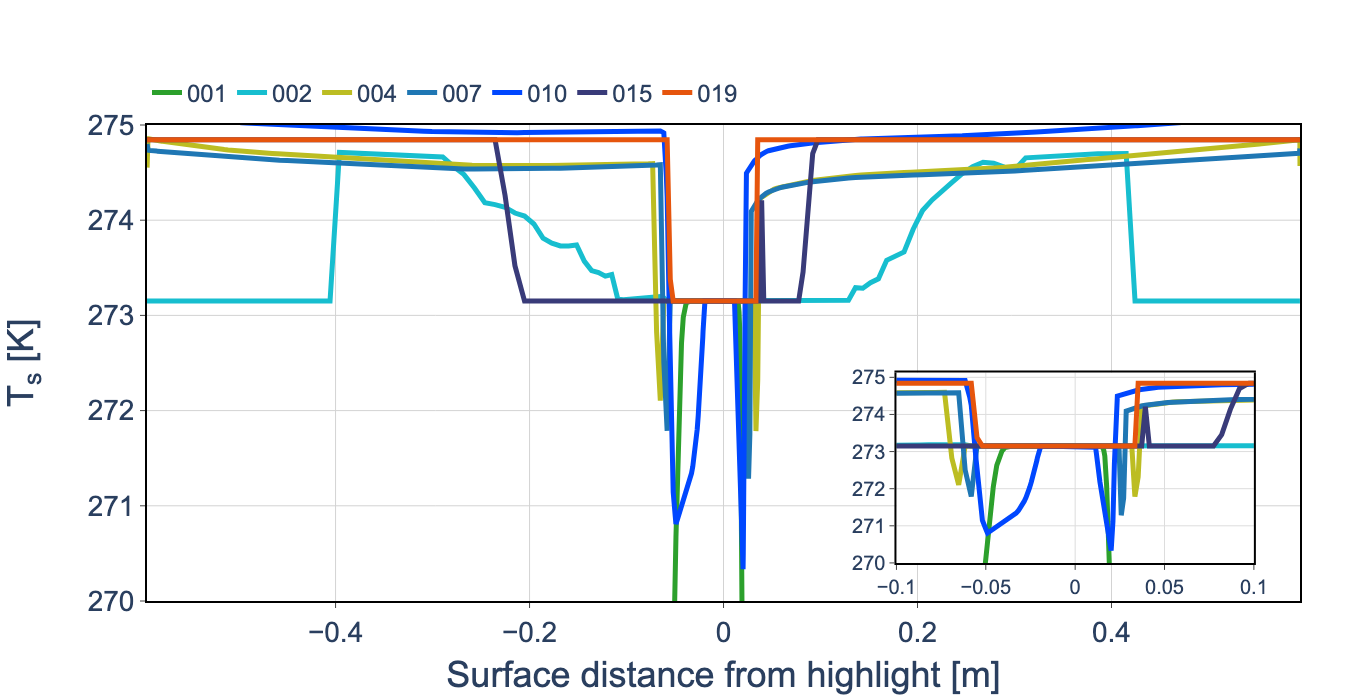
\includegraphics[width=0.94\textwidth]{FIGURES/SURF_TEMP_FF/tc_oneram6_L1_surface_temperature_vs_s_slice_1p4_roughness_1mm.png}

    \vspace{0.05cm}

    \textbf{$y=1.40$ m}
\end{column}

\end{columns}
}

\vspace{0.10cm}

\begin{block}{\scriptsize Observations}
\begin{itemize}
    \item<1-> Most submissions predict surface temperatures close to the freezing temperature over a large portion of the surface.
    \item<1-> Local code-to-code differences are concentrated near the leading edge.
    \item<2-> Similar differences are observed at the inboard and outboard spanwise stations.
\end{itemize}
\end{block}

\end{frame}


% ============================================================
% ONERA M6 -- Mean Surface Temperature
% ============================================================

\begin{frame}{\small ONERA M6 -- Mean Surface Temperature Grid Convergence}
\scriptsize

% ------------------------------------------------------------
% Middle slice -- 1 mm roughness
% ------------------------------------------------------------
\only<1>{
\begin{columns}[T,onlytextwidth]

\begin{column}{0.50\textwidth}
    \centering
    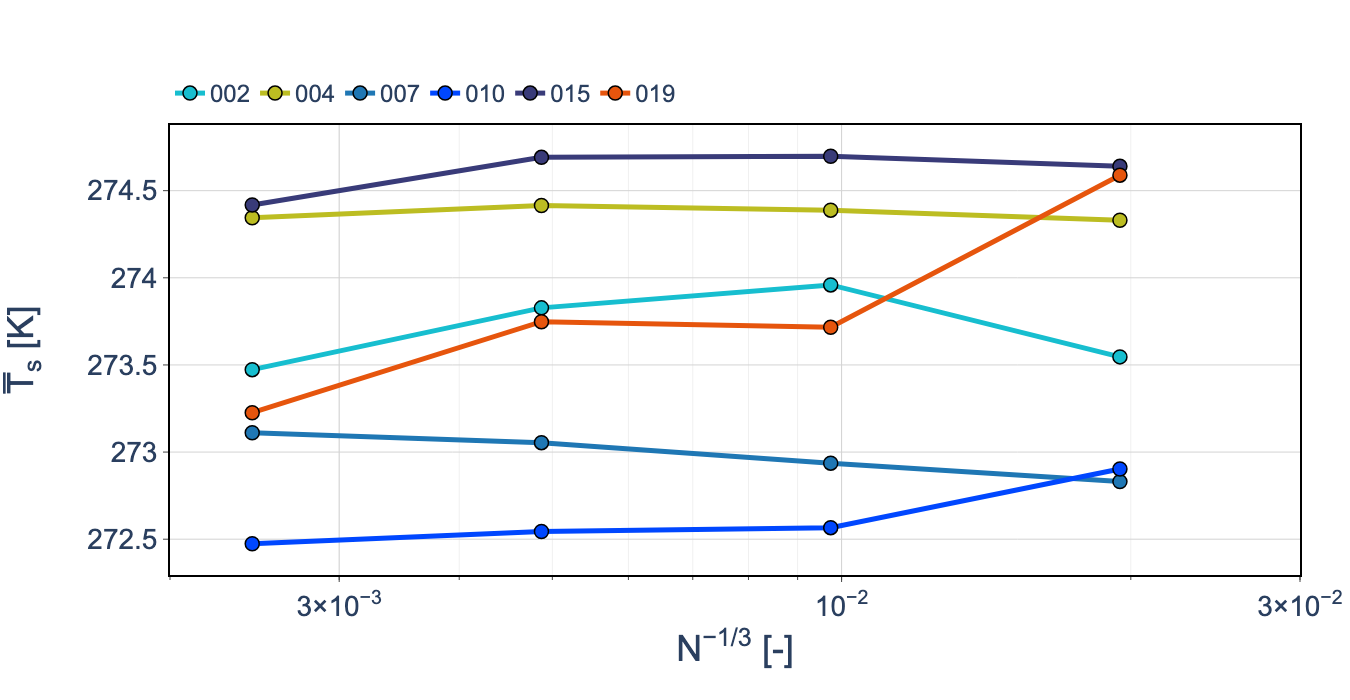
\includegraphics[width=0.94\textwidth]{FIGURES/SURF_TEMP_FF/tc_oneram6_mean_surface_temperature_vs_n_slice_0p75_roughness_1mm.png}

    \vspace{0.05cm}
\end{column}

\begin{column}{0.50\textwidth}
    \centering
    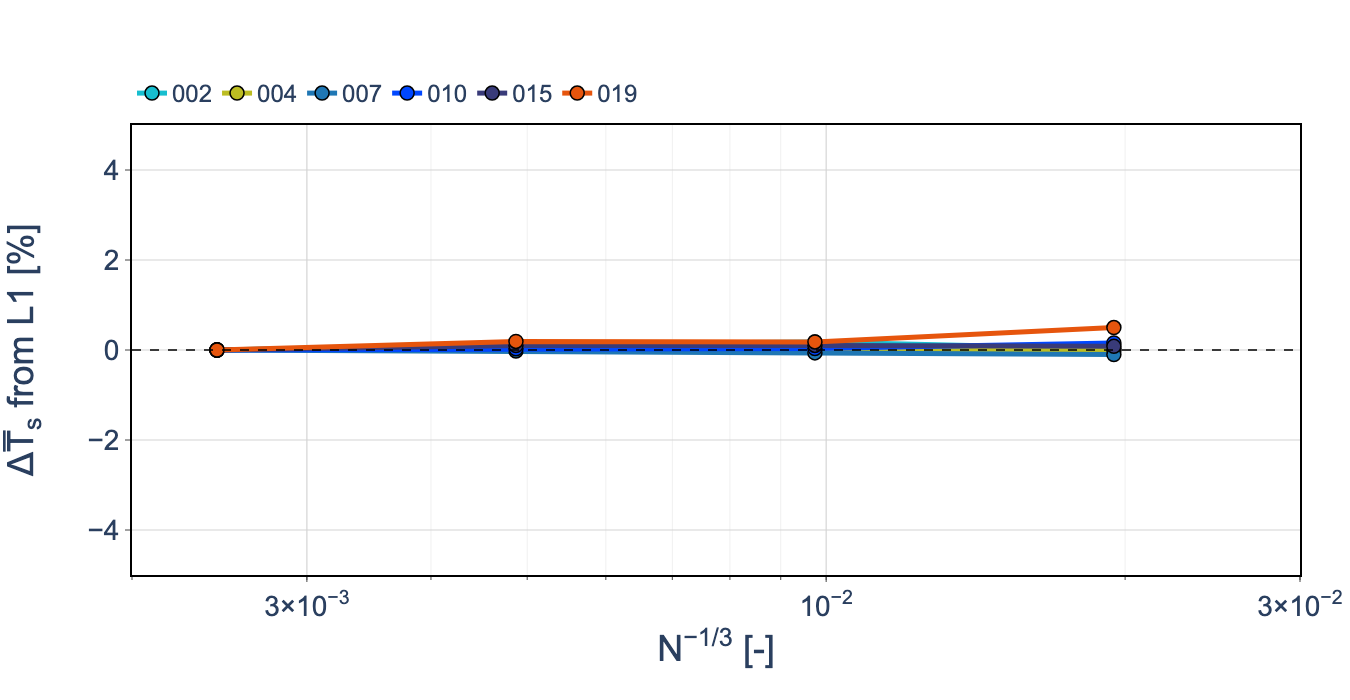
\includegraphics[width=0.94\textwidth]{FIGURES/SURF_TEMP_FF/tc_oneram6_mean_surface_temperature_vs_n_slice_0p75_roughness_1mm_relative_to_l1.png}

    \vspace{0.05cm}

\end{column}

\end{columns}

\vspace{0.05cm}

\centering
\textbf{$y=0.75$ m}
}

% ------------------------------------------------------------
% Inboard and outboard slices -- 1 mm roughness
% ------------------------------------------------------------
\only<2>{
\begin{columns}[T,onlytextwidth]

\begin{column}{0.50\textwidth}
    \centering
    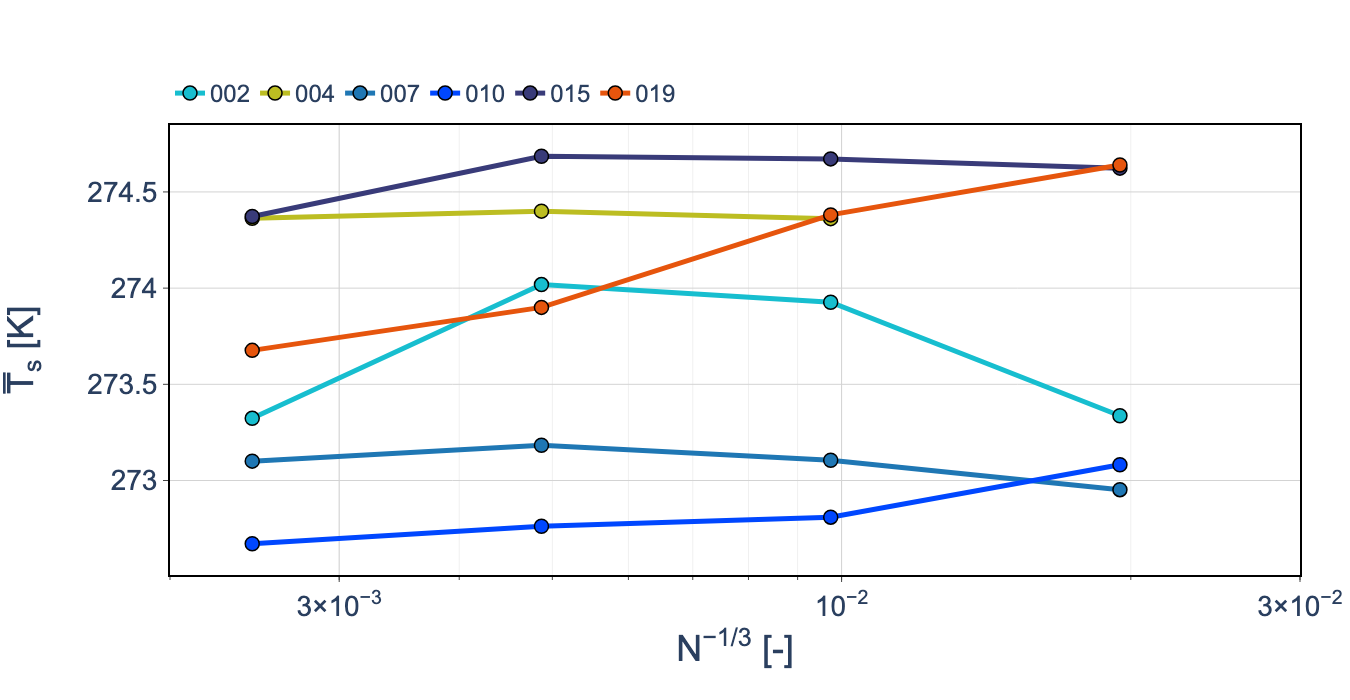
\includegraphics[width=0.94\textwidth]{FIGURES/SURF_TEMP_FF/tc_oneram6_mean_surface_temperature_vs_n_slice_0p1_roughness_1mm.png}

    \vspace{0.05cm}

    \textbf{$y=0.10$ m}
\end{column}

\begin{column}{0.50\textwidth}
    \centering
    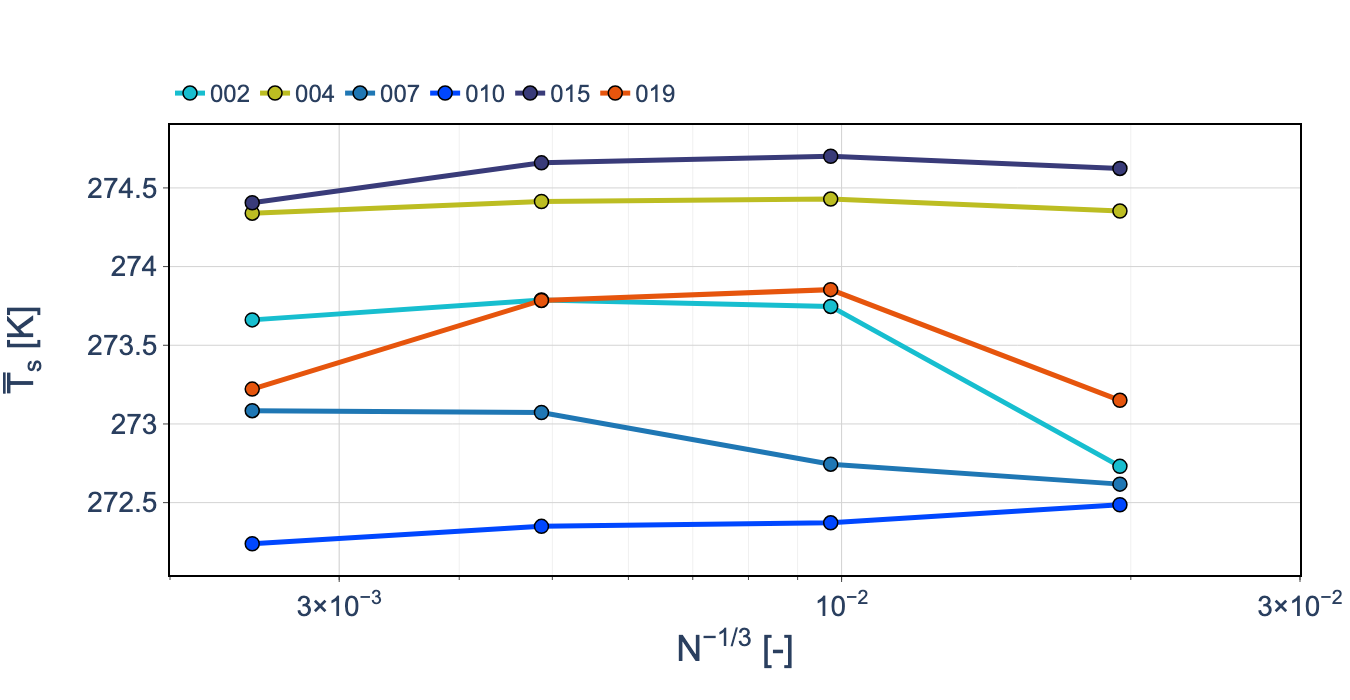
\includegraphics[width=0.94\textwidth]{FIGURES/SURF_TEMP_FF/tc_oneram6_mean_surface_temperature_vs_n_slice_1p4_roughness_1mm.png}

    \vspace{0.05cm}

    \textbf{$y=1.40$ m}
\end{column}

\end{columns}
}

% ------------------------------------------------------------
% Middle slice -- roughness sensitivity
% ------------------------------------------------------------
\only<3>{
\centering
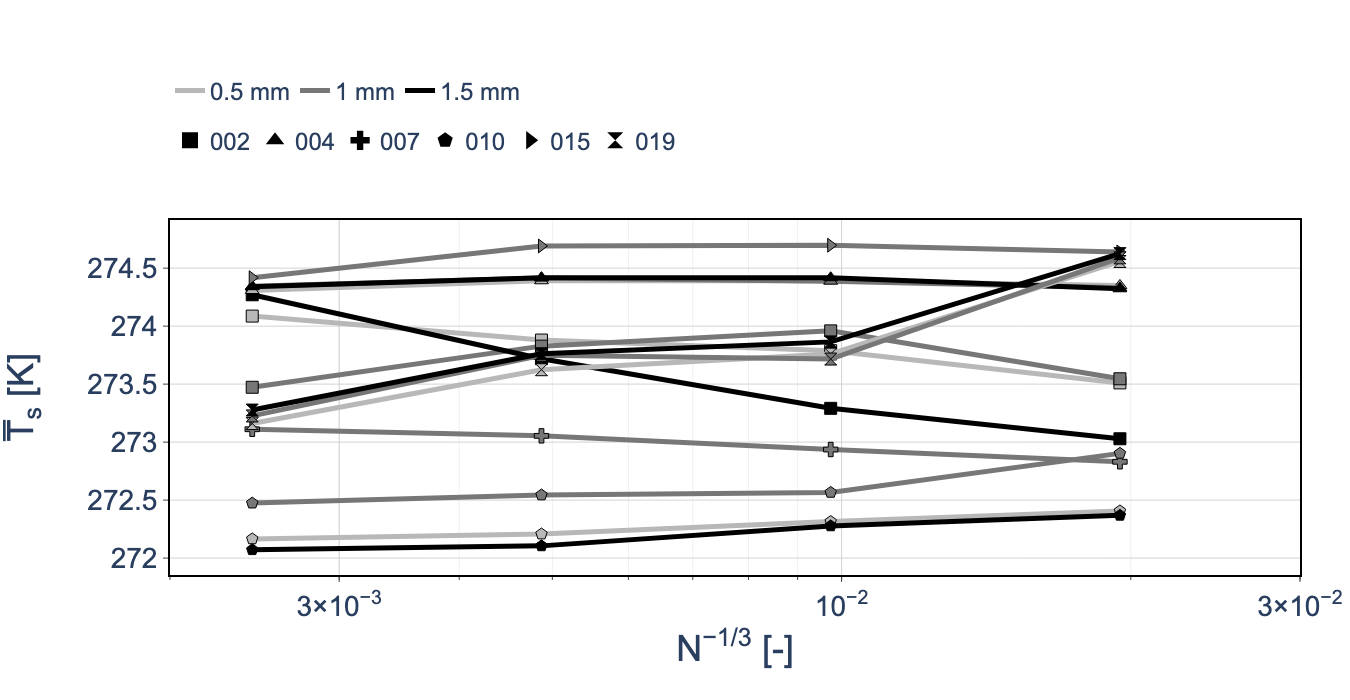
\includegraphics[width=0.5\textwidth]{FIGURES/SURF_TEMP_FF/tc_oneram6_mean_surface_temperature_vs_n_slice_0p75_grouped_roughness.png}

\vspace{0.05cm}

\textbf{$y=0.75$ m}
}

\vspace{0.10cm}

\begin{block}{\scriptsize Observations}
\begin{itemize}
    \item<1-> Mean $T_s$ is area-weighted ($ds$) over the iced surface ($h_{\mathrm{ice}}>0$).
    \item<1-> Grid sensitivity is limited ($<1\%$ for most submissions), with closely clustered predictions.
    \item<2-> Similar behavior is observed across the spanwise stations.
    \item<3-> Roughness changes mean $T_s$ by approximately $\pm1$ K, with a code-dependent response.
\end{itemize}
\end{block}

\end{frame}

% ============================================================
% ONERA M6 -- Participant-Level Roughness Sensitivity
% ============================================================

\begin{frame}{\small ONERA M6 -- Participant-Level Mean Surface Temperature Roughness Sensitivity (L1)}
\scriptsize
\vspace{-0.2cm}
\centering
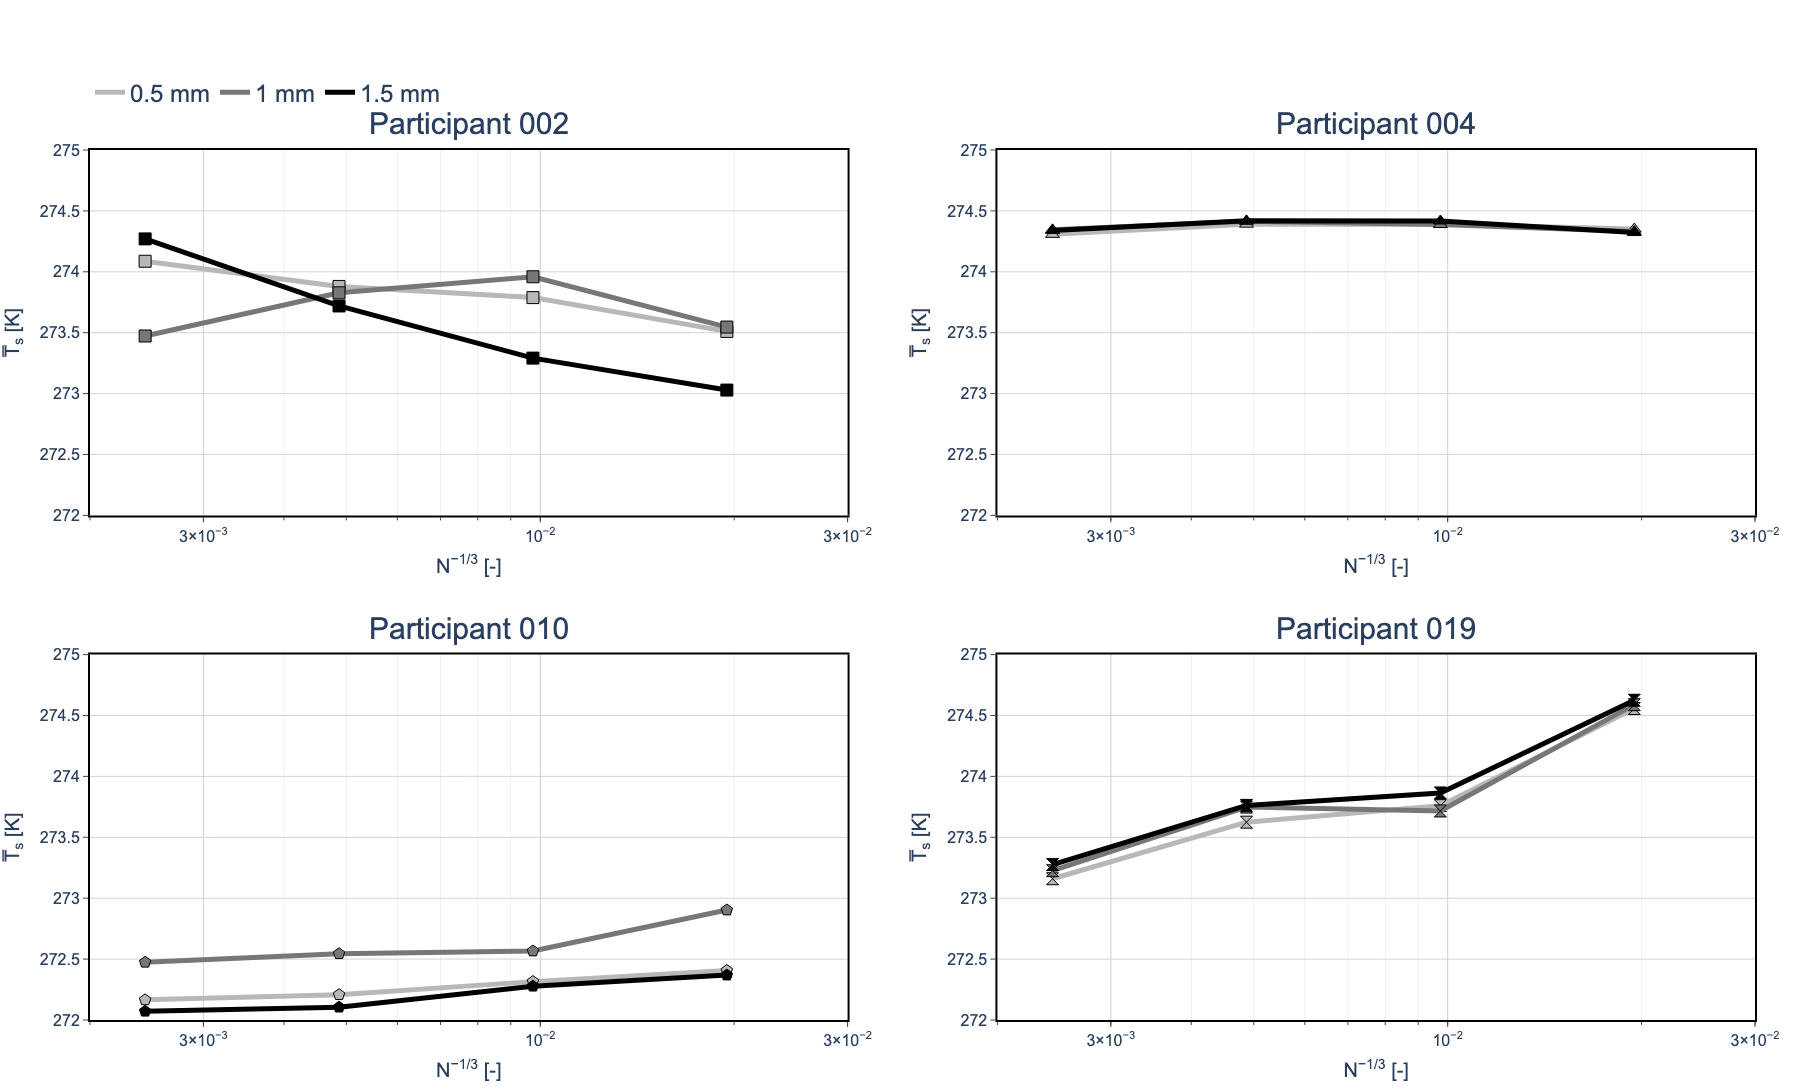
\includegraphics[width=0.8\textwidth]{FIGURES/SURF_TEMP_FF/tc_oneram6_mean_surface_temperature_vs_n_slice_0p75_grouped_roughness_participants.png}

\end{frame}

% ============================================================
% ONERA M6 -- Integrated Convective Heat Transfer
% ============================================================

\begin{frame}[shrink=15]{\small ONERA M6 -- Integrated Convective Heat Transfer}
\scriptsize

\centering

\begin{minipage}{0.90\textwidth}
\begin{block}{\scriptsize Grid-Convergence Metric}
To assess whether the differences in the local $HTC$ distributions translate
into a clear grid-convergence behavior, an integrated convective heat-transfer
quantity is evaluated along the surface slice:
\[
\boxed{
Q_c'
=
\int
HTC(s)
\left[
T_s(s)-T_{\mathrm{rec}}(s)
\right]\,ds
}
\qquad
[Q_c'] = \mathrm{W/m}.
\]

The submitted $HTC$ and surface temperature $T_s$ are used directly.
The recovery temperature $T_{\mathrm{rec}}$, however, was not part of the
submitted dataset and must therefore be reconstructed.
\end{block}
\end{minipage}

\vspace{0.15cm}

\begin{minipage}{0.90\textwidth}
\begin{block}{\scriptsize Recovery Temperature Reconstruction}
The submitted pressure coefficient is used to estimate the local external-flow
state and subsequently the recovery temperature:
\[
\boxed{
C_p(s)
\;\longrightarrow\;
p_e(s)
\;\longrightarrow\;
M_e(s)
\;\longrightarrow\;
T_e(s)
\;\longrightarrow\;
T_{\mathrm{rec}}(s)
}
\]

Assuming $p_s \simeq p_e$ and an isentropic external flow,
\[
\frac{p_e}{p_\infty}
=
1+\frac{\gamma}{2}M_\infty^2 C_{p,e},
\qquad
M_e^2
=
\frac{2}{\gamma-1}
\left[
\left(\frac{p_0}{p_e}\right)^{(\gamma-1)/\gamma}-1
\right],
\]
\[
T_e
=
\frac{T_0}
{1+\dfrac{\gamma-1}{2}M_e^2},
\qquad
T_{\mathrm{rec}}
=
T_e
\left[
1+r\frac{\gamma-1}{2}M_e^2
\right],
\qquad
r=Pr^{1/3}\approx0.9.
\]

\end{block}
\end{minipage}

\end{frame}

% ============================================================
% ONERA M6 -- Recovery Temperature Distribution
% ============================================================

\begin{frame}{\small ONERA M6 -- Reconstructed Recovery Temperature Distribution (L1)}
\scriptsize

% ------------------------------------------------------------
% Middle slice
% ------------------------------------------------------------
\only<1>{
\centering
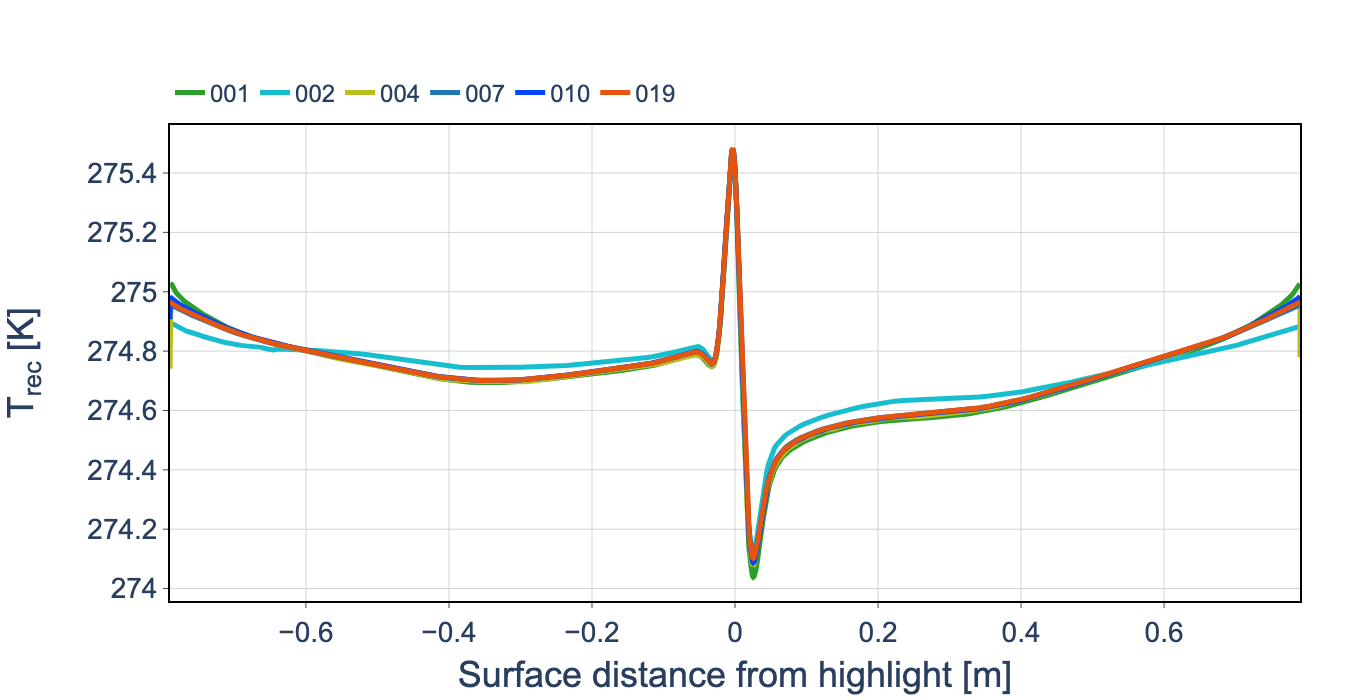
\includegraphics[width=0.5\textwidth]{FIGURES/HTC/tc_oneram6_L1_recovery_temperature_vs_s_slice_0p75_roughness_1mm.png}

\vspace{0.05cm}

\textbf{$y=0.75$ m}
}

% ------------------------------------------------------------
% Inboard and outboard slices
% ------------------------------------------------------------
\only<2>{
\begin{columns}[T,onlytextwidth]

\begin{column}{0.50\textwidth}
    \centering
    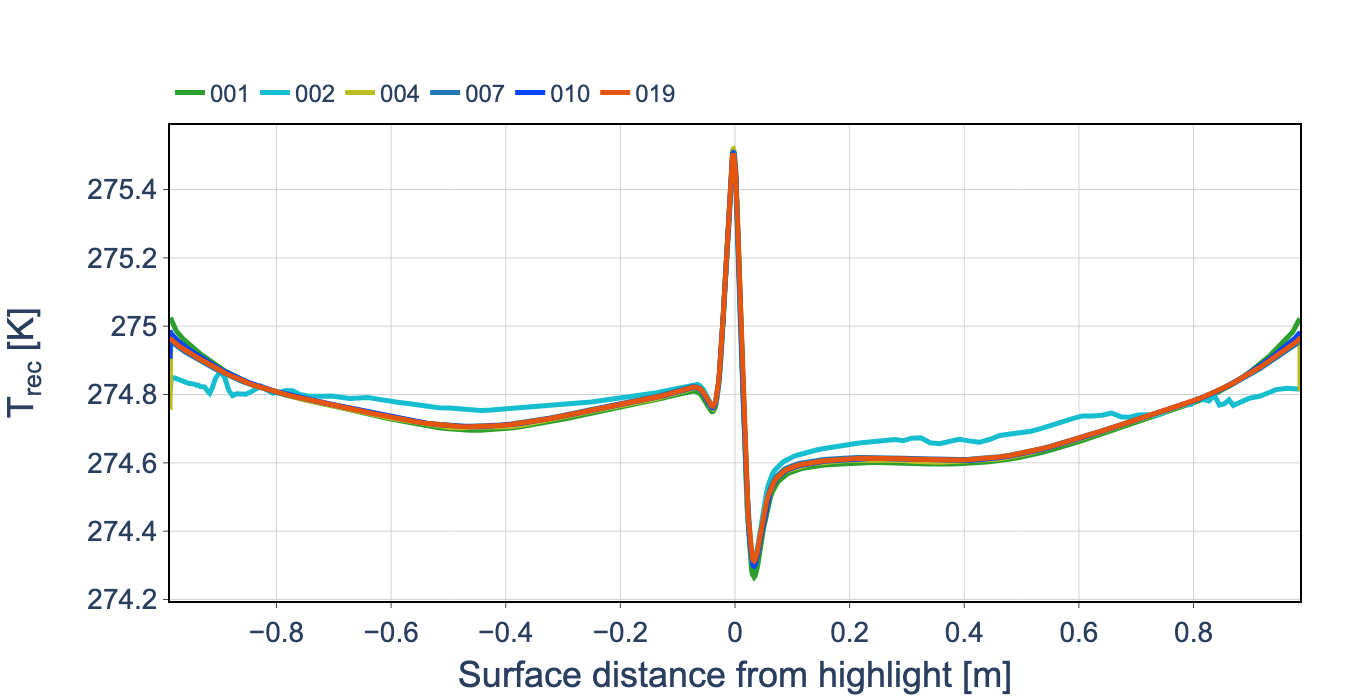
\includegraphics[width=0.92\textwidth]{FIGURES/HTC/tc_oneram6_L1_recovery_temperature_vs_s_slice_0p1_roughness_1mm.png}

    \vspace{0.05cm}

    \textbf{$y=0.10$ m}
\end{column}

\begin{column}{0.50\textwidth}
    \centering
    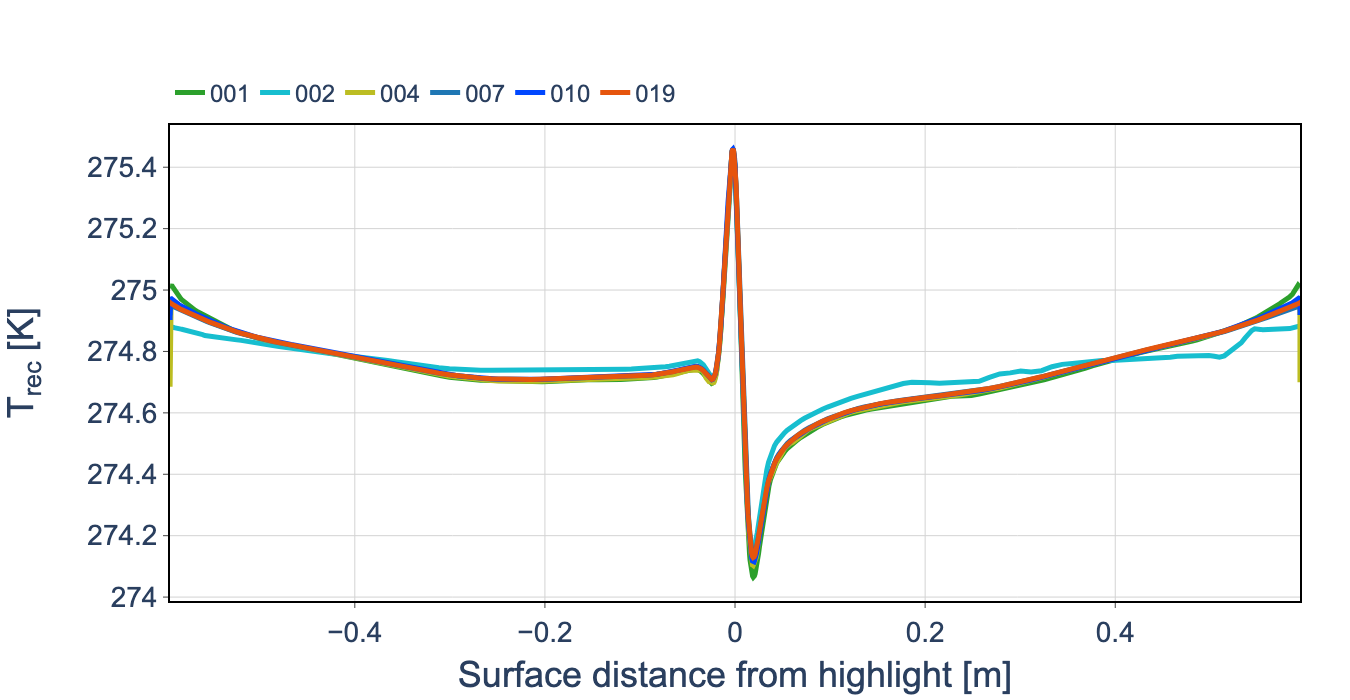
\includegraphics[width=0.92\textwidth]{FIGURES/HTC/tc_oneram6_L1_recovery_temperature_vs_s_slice_1p4_roughness_1mm.png}

    \vspace{0.05cm}

    \textbf{$y=1.40$ m}
\end{column}

\end{columns}
}

\vspace{0.05cm}

\begin{block}{\scriptsize Observations}
\begin{itemize}
    \item<1-> The reconstructed recovery-temperature distributions are closely aligned across submissions.
    \item<1-> This agreement is consistent with the good code-to-code agreement previously observed for $C_p$, from which $T_{\mathrm{rec}}$ is reconstructed.
    \item<2-> Similar agreement is observed at the inboard and outboard spanwise stations.
\end{itemize}
\end{block}

\end{frame}

% ============================================================
% ONERA M6 -- Convective Heat Transfer Grid Convergence
% ============================================================

\begin{frame}{\small ONERA M6 -- Convective Heat Transfer Grid Convergence}
\scriptsize

% ------------------------------------------------------------
% Middle slice -- absolute and relative to L1
% ------------------------------------------------------------
\only<1>{
\begin{columns}[T,onlytextwidth]

\begin{column}{0.50\textwidth}
    \centering
    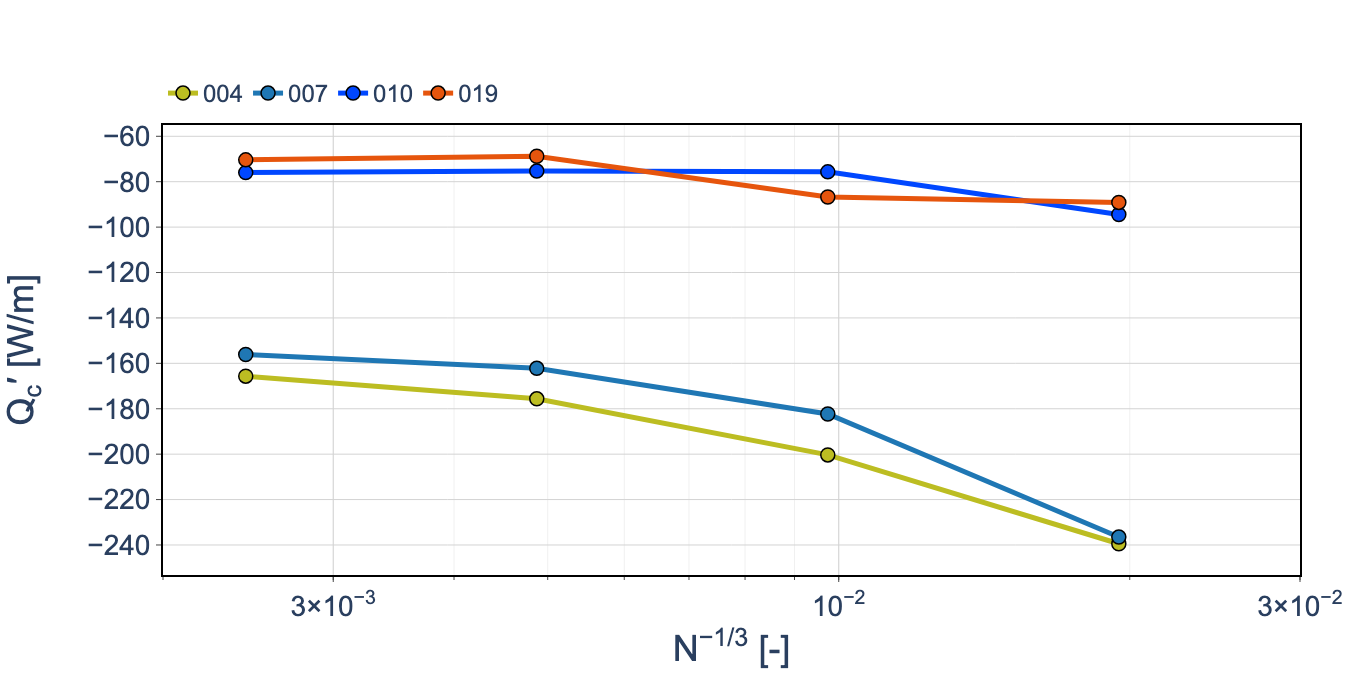
\includegraphics[width=0.94\textwidth]{FIGURES/HTC/tc_oneram6_qc_prime_vs_n_y_0.75.png}
\end{column}

\begin{column}{0.50\textwidth}
    \centering
    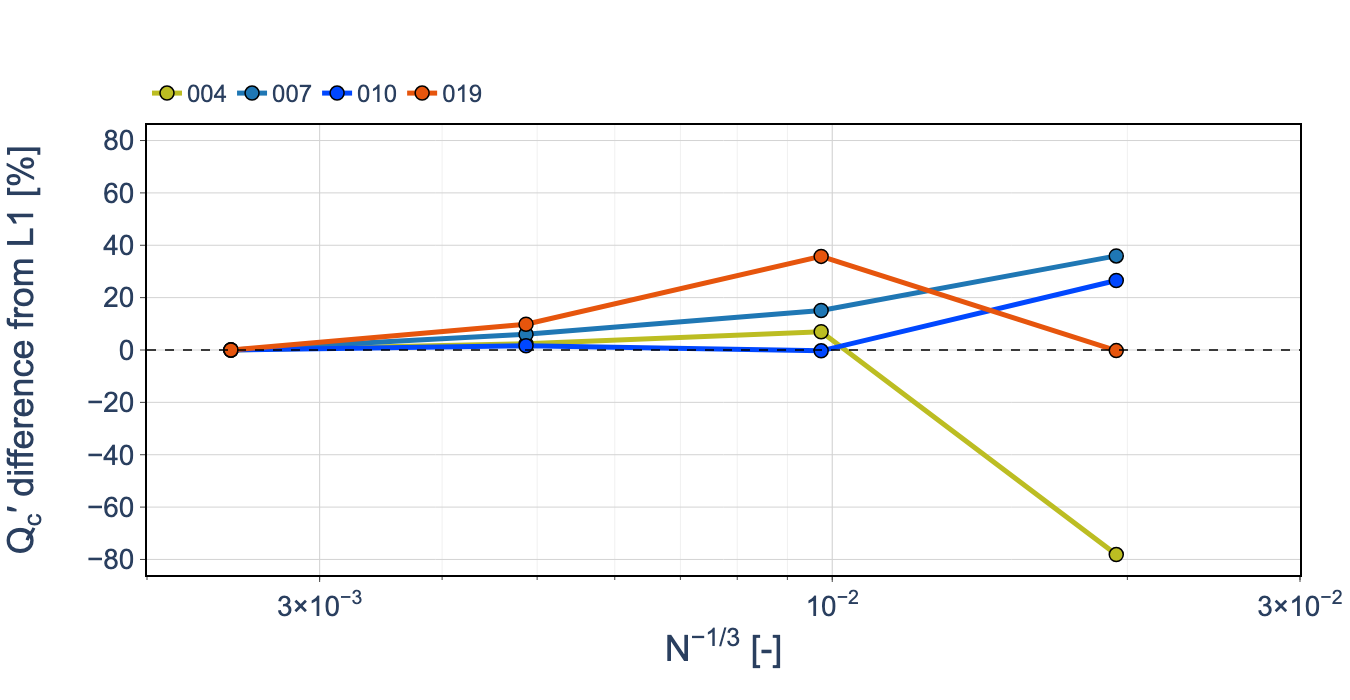
\includegraphics[width=0.94\textwidth]{FIGURES/HTC/tc_oneram6_qc_prime_vs_n_y_0.1_relative_to_l1.png}
\end{column}

\end{columns}

\vspace{0.05cm}

\centering
\textbf{$y=0.75$ m}
}

% ------------------------------------------------------------
% Inboard and outboard slices -- 1 mm roughness
% ------------------------------------------------------------
\only<2>{
\begin{columns}[T,onlytextwidth]

\begin{column}{0.50\textwidth}
    \centering
    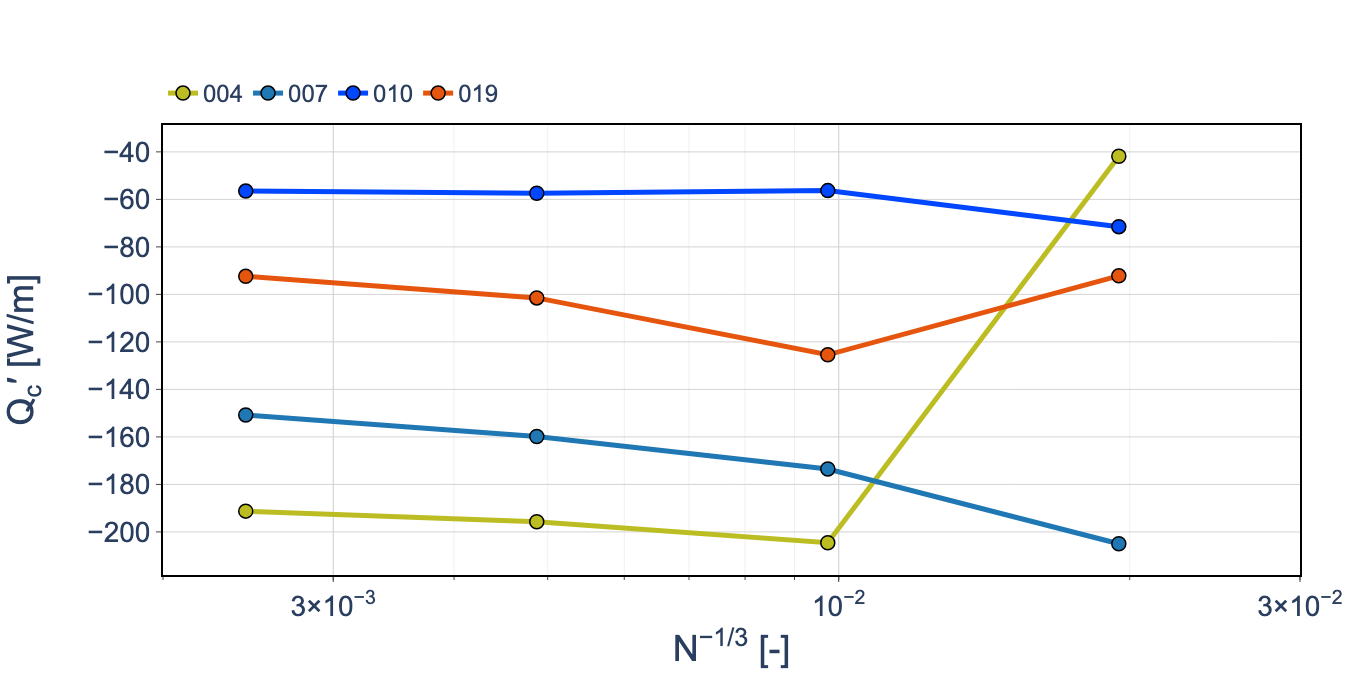
\includegraphics[width=0.94\textwidth]{FIGURES/HTC/tc_oneram6_qc_prime_vs_n_y_0.1.png}

    \vspace{0.05cm}

    \textbf{$y=0.10$ m}
\end{column}

\begin{column}{0.50\textwidth}
    \centering
    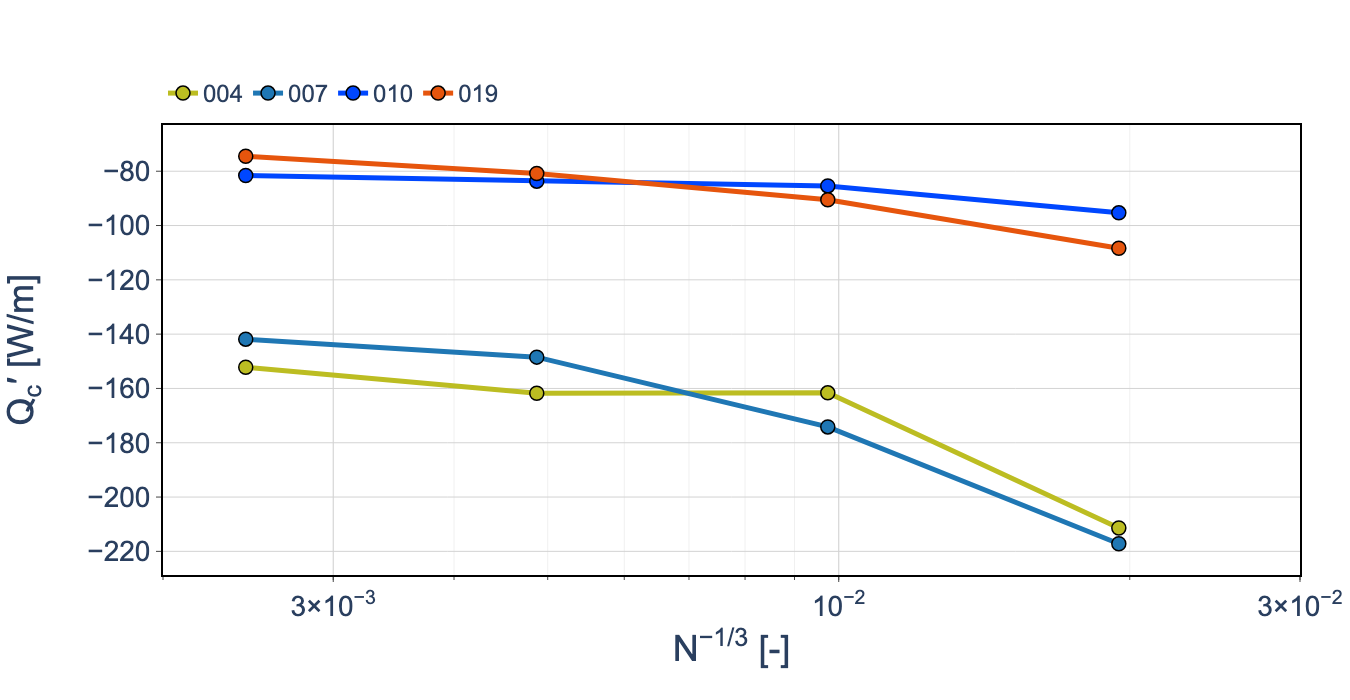
\includegraphics[width=0.94\textwidth]{FIGURES/HTC/tc_oneram6_qc_prime_vs_n_y_1.4.png}

    \vspace{0.05cm}

    \textbf{$y=1.40$ m}
\end{column}

\end{columns}
}

% ------------------------------------------------------------
% Middle slice -- roughness sensitivity
% ------------------------------------------------------------
\only<3>{
\centering
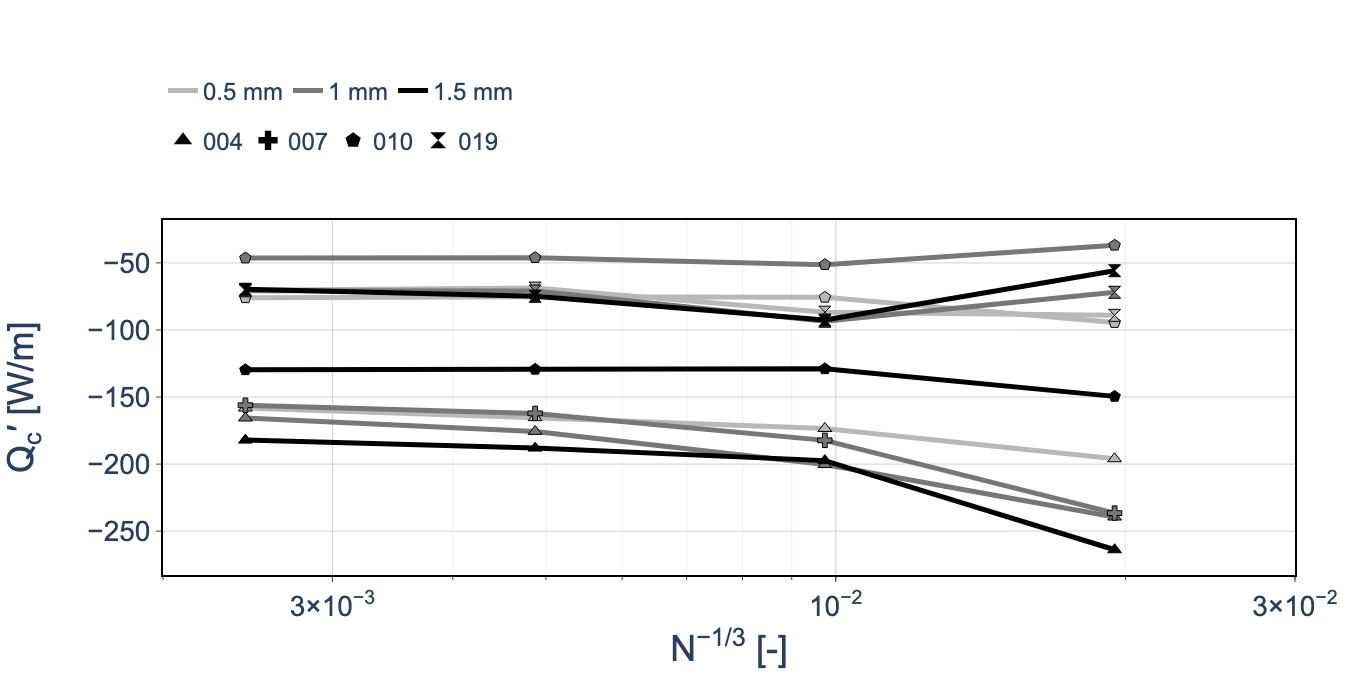
\includegraphics[width=0.5\textwidth]{FIGURES/HTC/tc_oneram6_qc_prime_vs_n_y_0.75_grouped_roughness.png}

\vspace{0.05cm}

\textbf{$y=0.75$ m- Roughness Sensitivity}
}

\vspace{0.10cm}

\begin{block}{\scriptsize Observations}
\begin{itemize}
    \item<1-> Considerable code-to-code variability is observed in $Q_c'$, exceeding the L1--L2 grid effect for most submissions.
    \item<2-> Large variability persists across all spanwise stations.
    \item<3-> Increasing surface roughness systematically increases $|Q_c'|$.
\end{itemize}
\end{block}

\end{frame}

% ============================================================
% ONERA M6 -- Participant-Level Roughness Sensitivity
% ============================================================

\begin{frame}{\small ONERA M6 -- Participant-Level HTC Roughness Sensitivity (L1)}
\scriptsize
\vspace{-0.2cm}
\centering
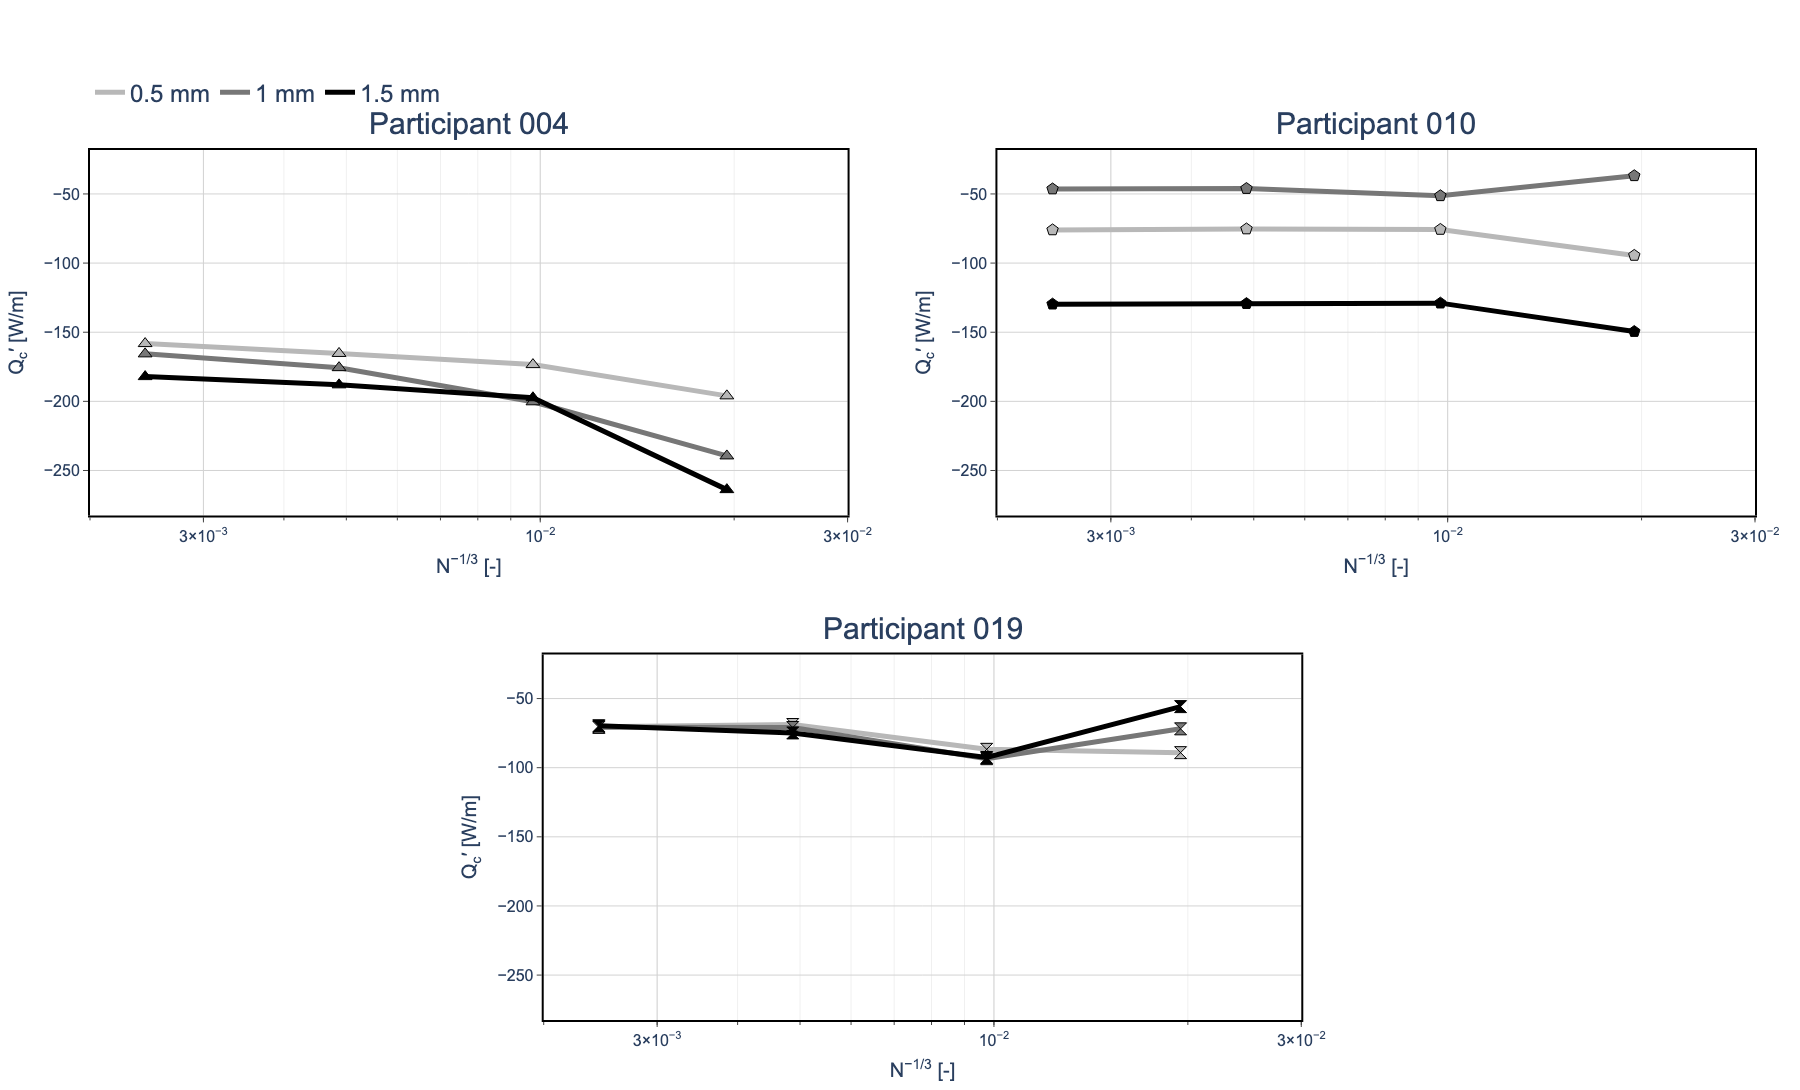
\includegraphics[width=0.8\textwidth]{FIGURES/HTC/tc_oneram6_qc_prime_vs_n_y_0.75_grouped_roughness_participants.png}

\end{frame}

% ============================================================
% ONERA M6 -- Freezing Fraction Distribution
% ============================================================

\begin{frame}{\small ONERA M6 -- Freezing-Fraction Distribution (L1)}
\scriptsize

% ------------------------------------------------------------
% Middle slice
% ------------------------------------------------------------
\only<1>{
\centering
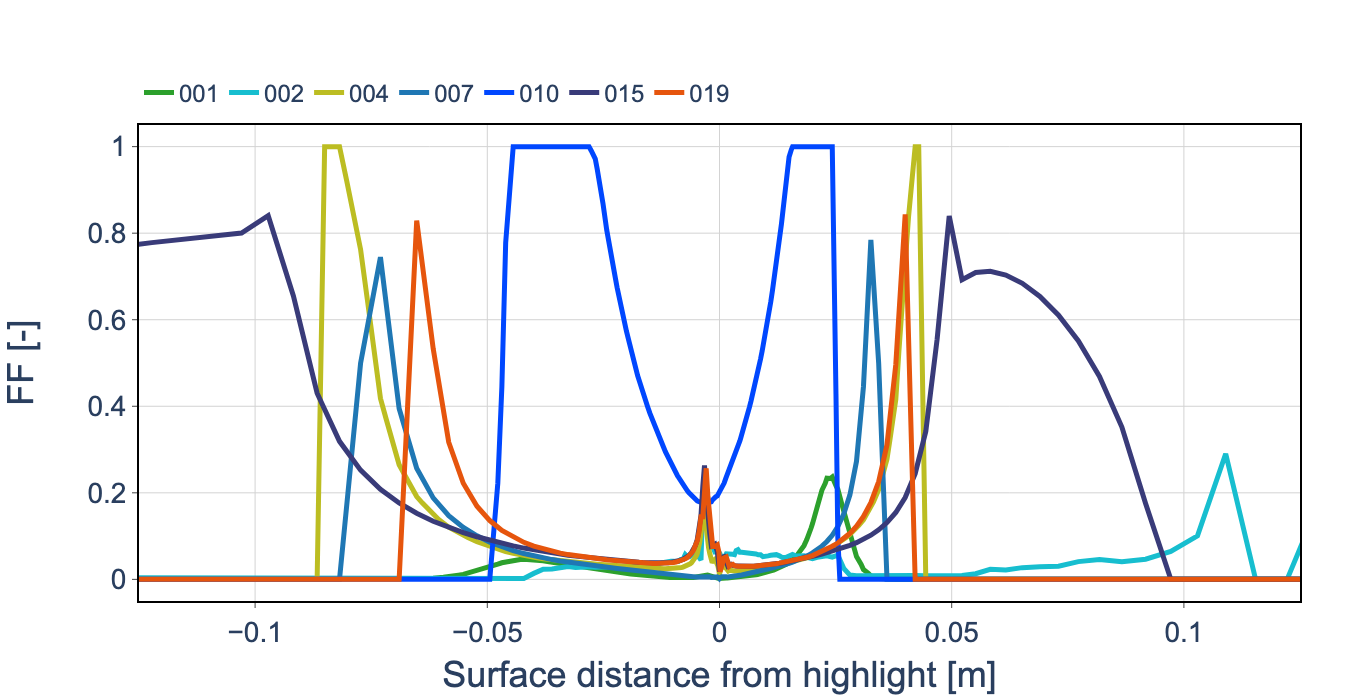
\includegraphics[width=0.5\textwidth]{FIGURES/SURF_TEMP_FF/tc_oneram6_L1_freezing_fraction_vs_s_slice_0p75_roughness_1mm.png}

\vspace{0.05cm}

\textbf{$y=0.75$ m}
}

% ------------------------------------------------------------
% Inboard and outboard slices
% ------------------------------------------------------------
\only<2>{
\begin{columns}[T,onlytextwidth]

\begin{column}{0.50\textwidth}
    \centering
    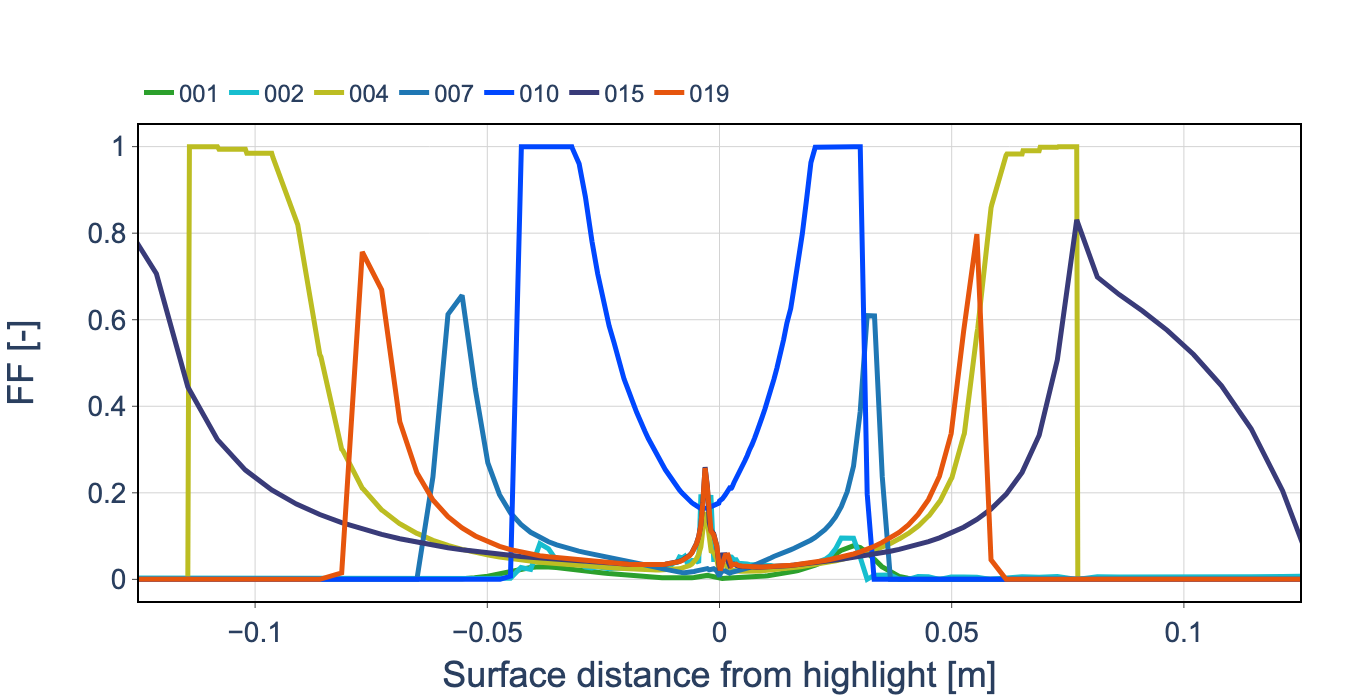
\includegraphics[width=0.94\textwidth]{FIGURES/SURF_TEMP_FF/tc_oneram6_L1_freezing_fraction_vs_s_slice_0p1_roughness_1mm.png}

    \vspace{0.05cm}

    \textbf{$y=0.10$ m}
\end{column}

\begin{column}{0.50\textwidth}
    \centering
    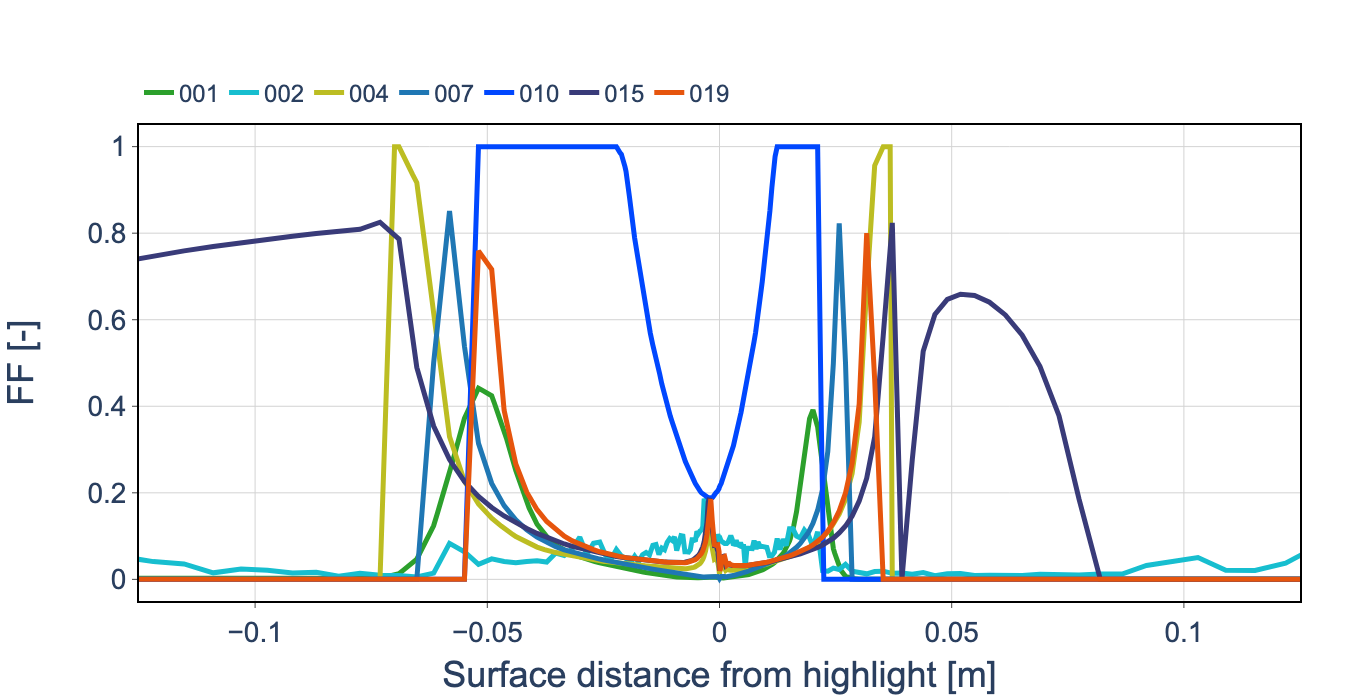
\includegraphics[width=0.94\textwidth]{FIGURES/SURF_TEMP_FF/tc_oneram6_L1_freezing_fraction_vs_s_slice_1p4_roughness_1mm.png}

    \vspace{0.05cm}

    \textbf{$y=1.40$ m}
\end{column}

\end{columns}
}

\vspace{0.10cm}

\begin{block}{\scriptsize Observations}
\begin{itemize}
    \item<1-> Large code-to-code differences are observed in both the magnitude and spatial extent of the predicted freezing fraction.
    \item<2-> Substantial differences in the predicted freezing regime persist across the inboard and outboard spanwise stations.
    \item<2-> Roughness affects the extent of the ice-covered region, with both the magnitude and direction of the response varying between codes.
\end{itemize}
\end{block}

\end{frame}

% ============================================================
% ONERA M6 -- Participant-Level Roughness Sensitivity
% ============================================================

\begin{frame}{\small ONERA M6 -- Participant-Level Freezing Fraction Roughness Sensitivity (L1)}
\scriptsize
\vspace{-0.2cm}
\centering
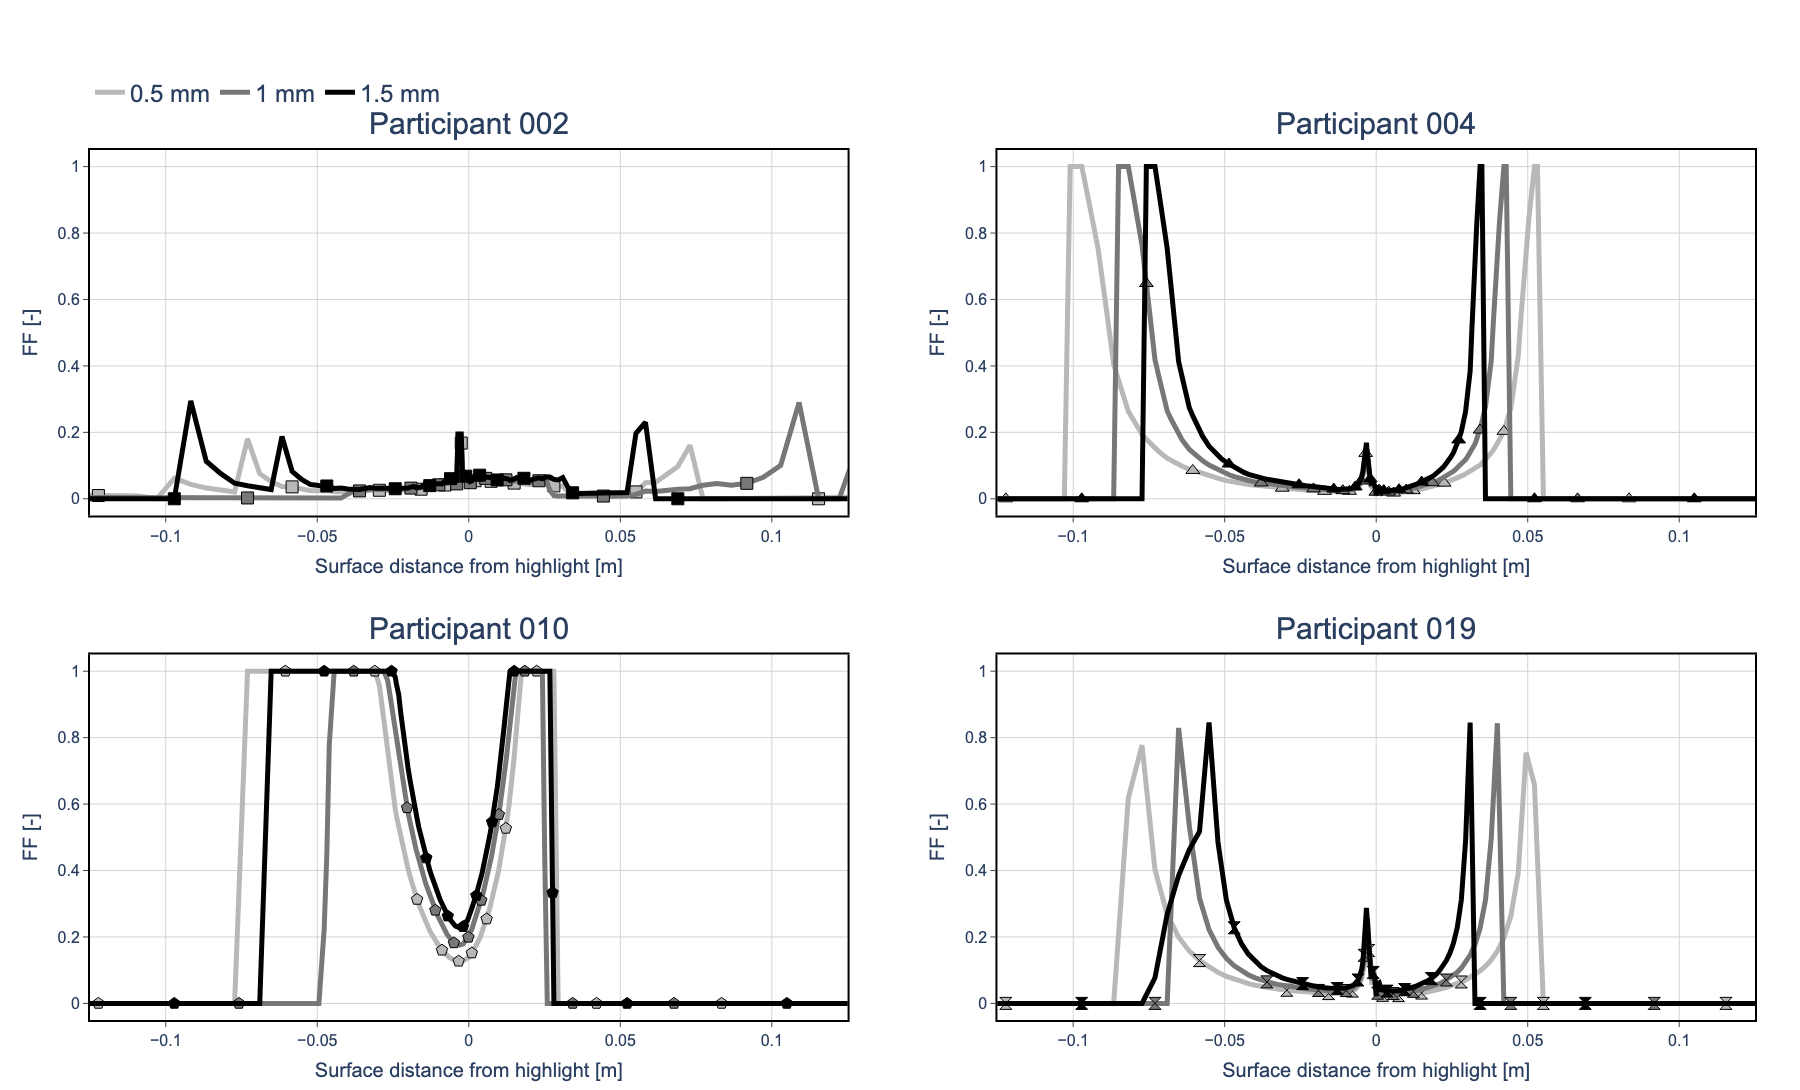
\includegraphics[width=0.7\textwidth]{FIGURES/SURF_TEMP_FF/tc_oneram6_L1_freezing_fraction_vs_s_slice_0p75_grouped_roughness_participants.png}

{\scriptsize\textbf{$y=0.75$ m -- Individual Participants}}

\end{frame}

% % ============================================================
% % ONERA M6 -- Mean Freezing Fraction
% % ============================================================

% \begin{frame}{\small ONERA M6 -- Mean Freezing Fraction Grid Convergence}
% \scriptsize

% % ------------------------------------------------------------
% % Middle slice -- 1 mm roughness
% % ------------------------------------------------------------
% \only<1>{
% \centering
% 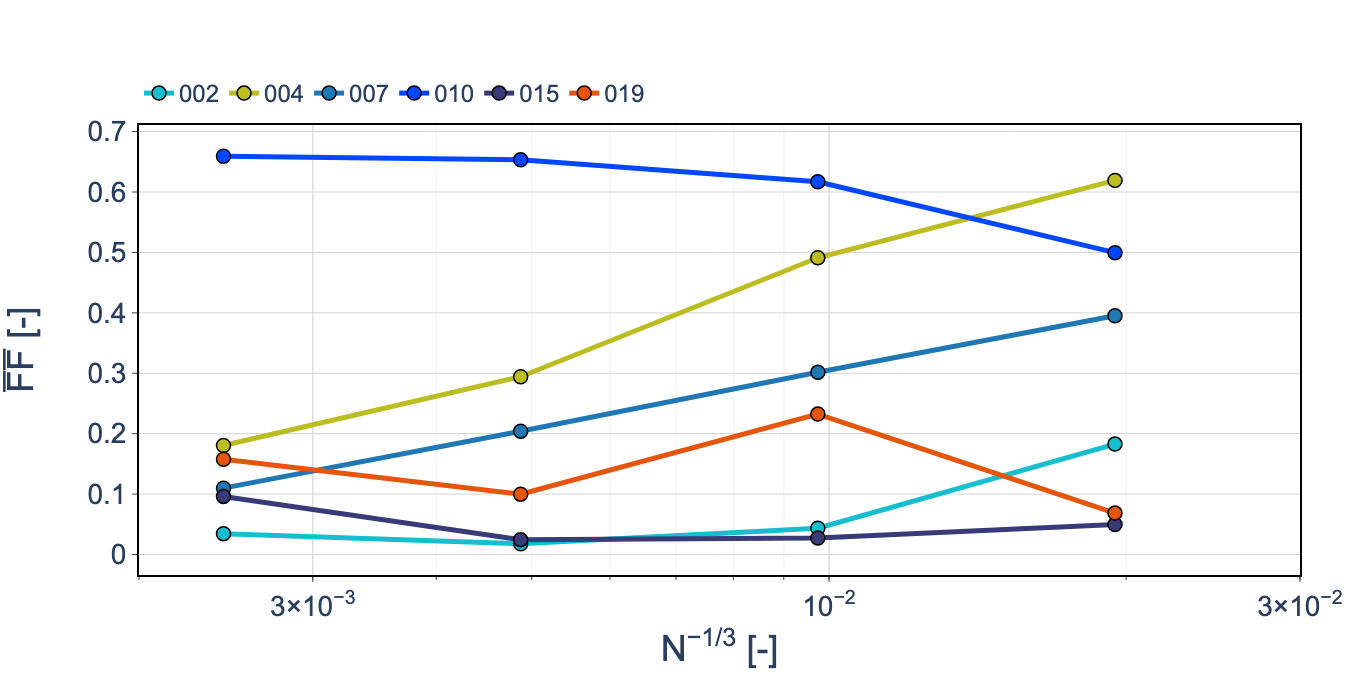
\includegraphics[width=0.5\textwidth]{FIGURES/SURF_TEMP_FF/tc_oneram6_mean_freezing_fraction_vs_n_slice_0p75_roughness_1mm.png}

% \vspace{0.05cm}

% \textbf{$y=0.75$ m}
% }

% % ------------------------------------------------------------
% % Inboard and outboard slices -- 1 mm roughness
% % ------------------------------------------------------------
% \only<2>{
% \begin{columns}[T,onlytextwidth]

% \begin{column}{0.50\textwidth}
%     \centering
%     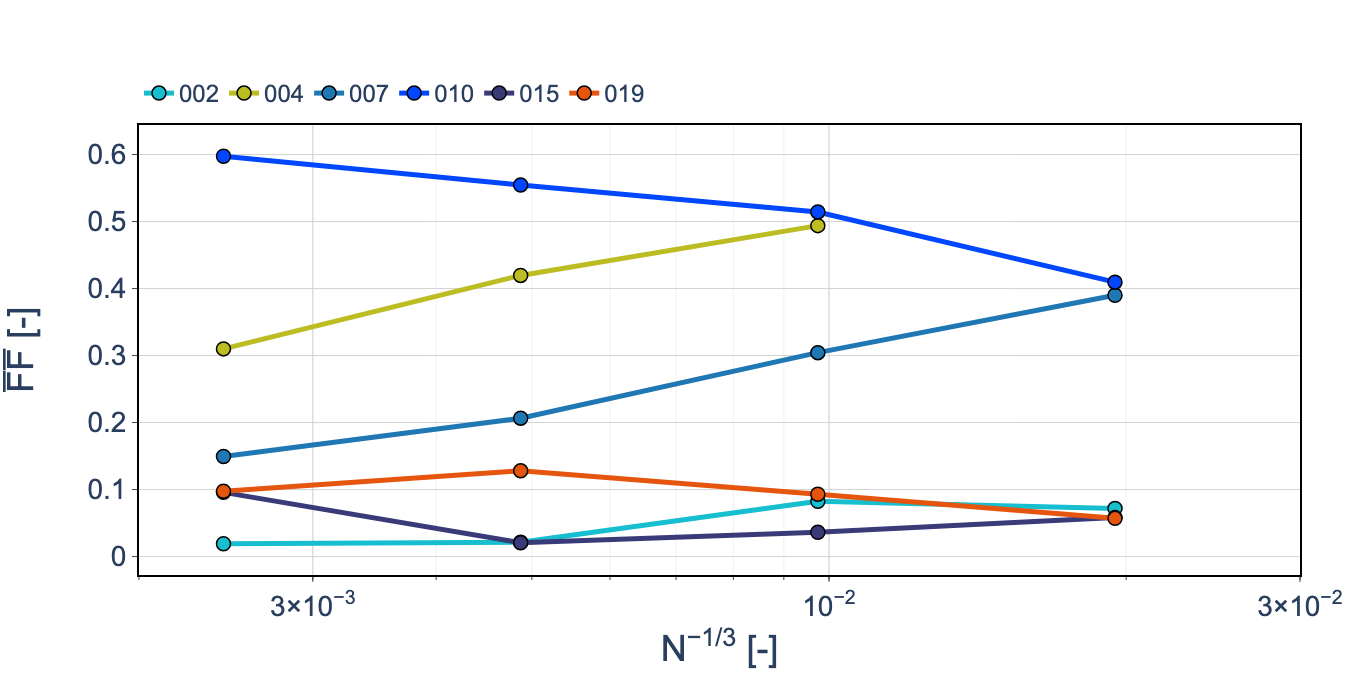
\includegraphics[width=0.94\textwidth]{FIGURES/SURF_TEMP_FF/tc_oneram6_mean_freezing_fraction_vs_n_slice_0p1_roughness_1mm.png}

%     \vspace{0.05cm}

%     \textbf{$y=0.10$ m}
% \end{column}

% \begin{column}{0.50\textwidth}
%     \centering
%     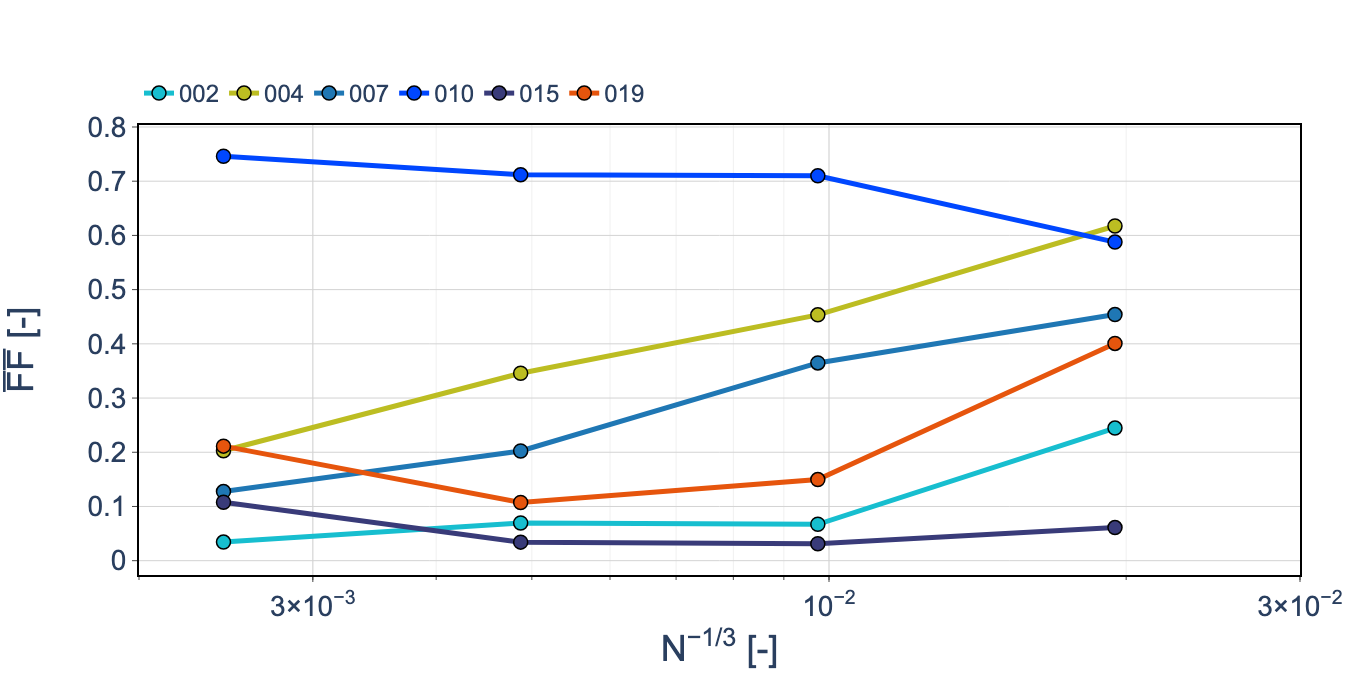
\includegraphics[width=0.94\textwidth]{FIGURES/SURF_TEMP_FF/tc_oneram6_mean_freezing_fraction_vs_n_slice_1p4_roughness_1mm.png}

%     \vspace{0.05cm}

%     \textbf{$y=1.40$ m}
% \end{column}

% \end{columns}
% }

% % ------------------------------------------------------------
% % Middle slice -- roughness sensitivity
% % ------------------------------------------------------------
% \only<3>{
% \centering
% 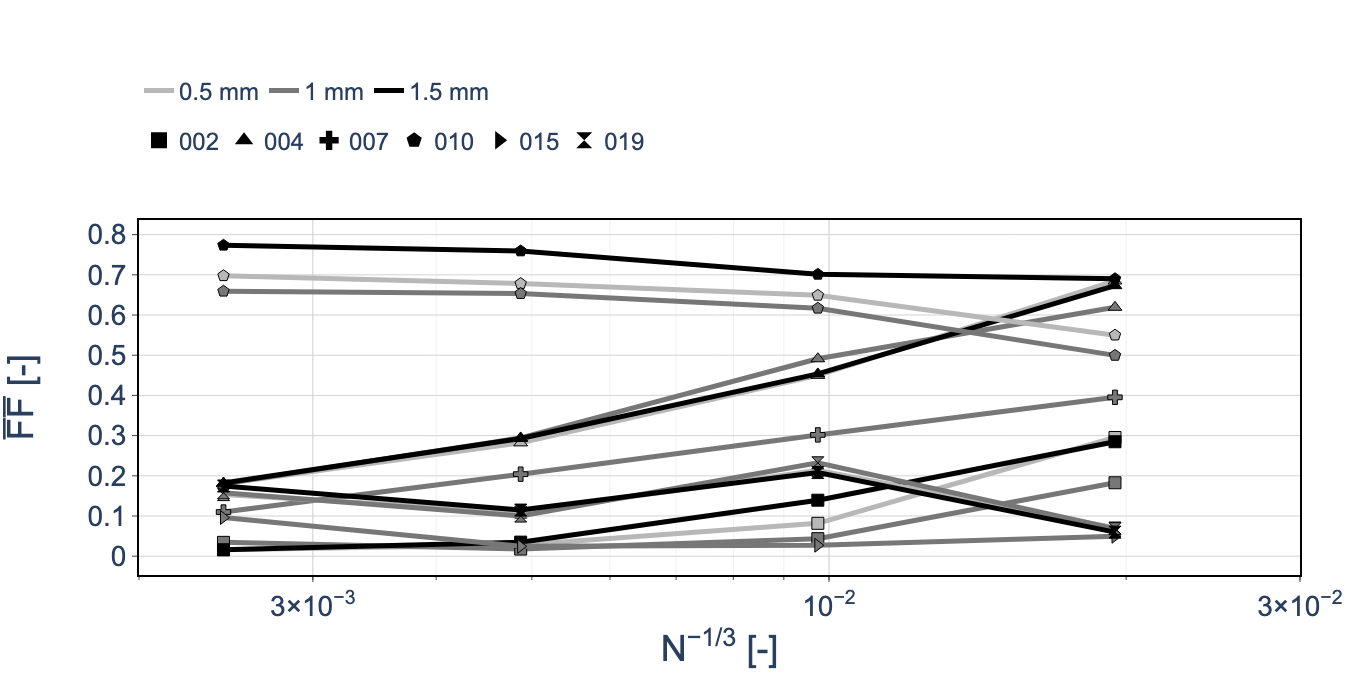
\includegraphics[width=0.5\textwidth]{FIGURES/SURF_TEMP_FF/tc_oneram6_mean_freezing_fraction_vs_n_slice_0p75_grouped_roughness.png}

% \vspace{0.05cm}

% \textbf{$y=0.75$ m- Roughness Sensitivity}
% }

% \vspace{0.10cm}

% \begin{block}{\scriptsize Observations}
% \begin{itemize}
%     \item<1-> Mean freezing fraction exhibits very large code-to-code variability, despite the comparatively close mean surface-temperature predictions for most submissions.
%     \item<1-> Grid sensitivity is submission-dependent, with some predictions remaining relatively stable while others vary substantially across the grid hierarchy.
%     \item<2-> Large code-to-code differences persist at the inboard and outboard spanwise stations.
%     \item<3-> Prescribed surface roughness introduces an additional systematic effect.
% \end{itemize}
% \end{block}

% \end{frame}

% % ============================================================
% % ONERA M6 -- Participant-Level Roughness Sensitivity
% % ============================================================

% \begin{frame}{\small ONERA M6 -- Participant-Level Freezing Fraction Roughness Sensitivity (L1)}
% \scriptsize
% \vspace{-0.2cm}
% \centering
% 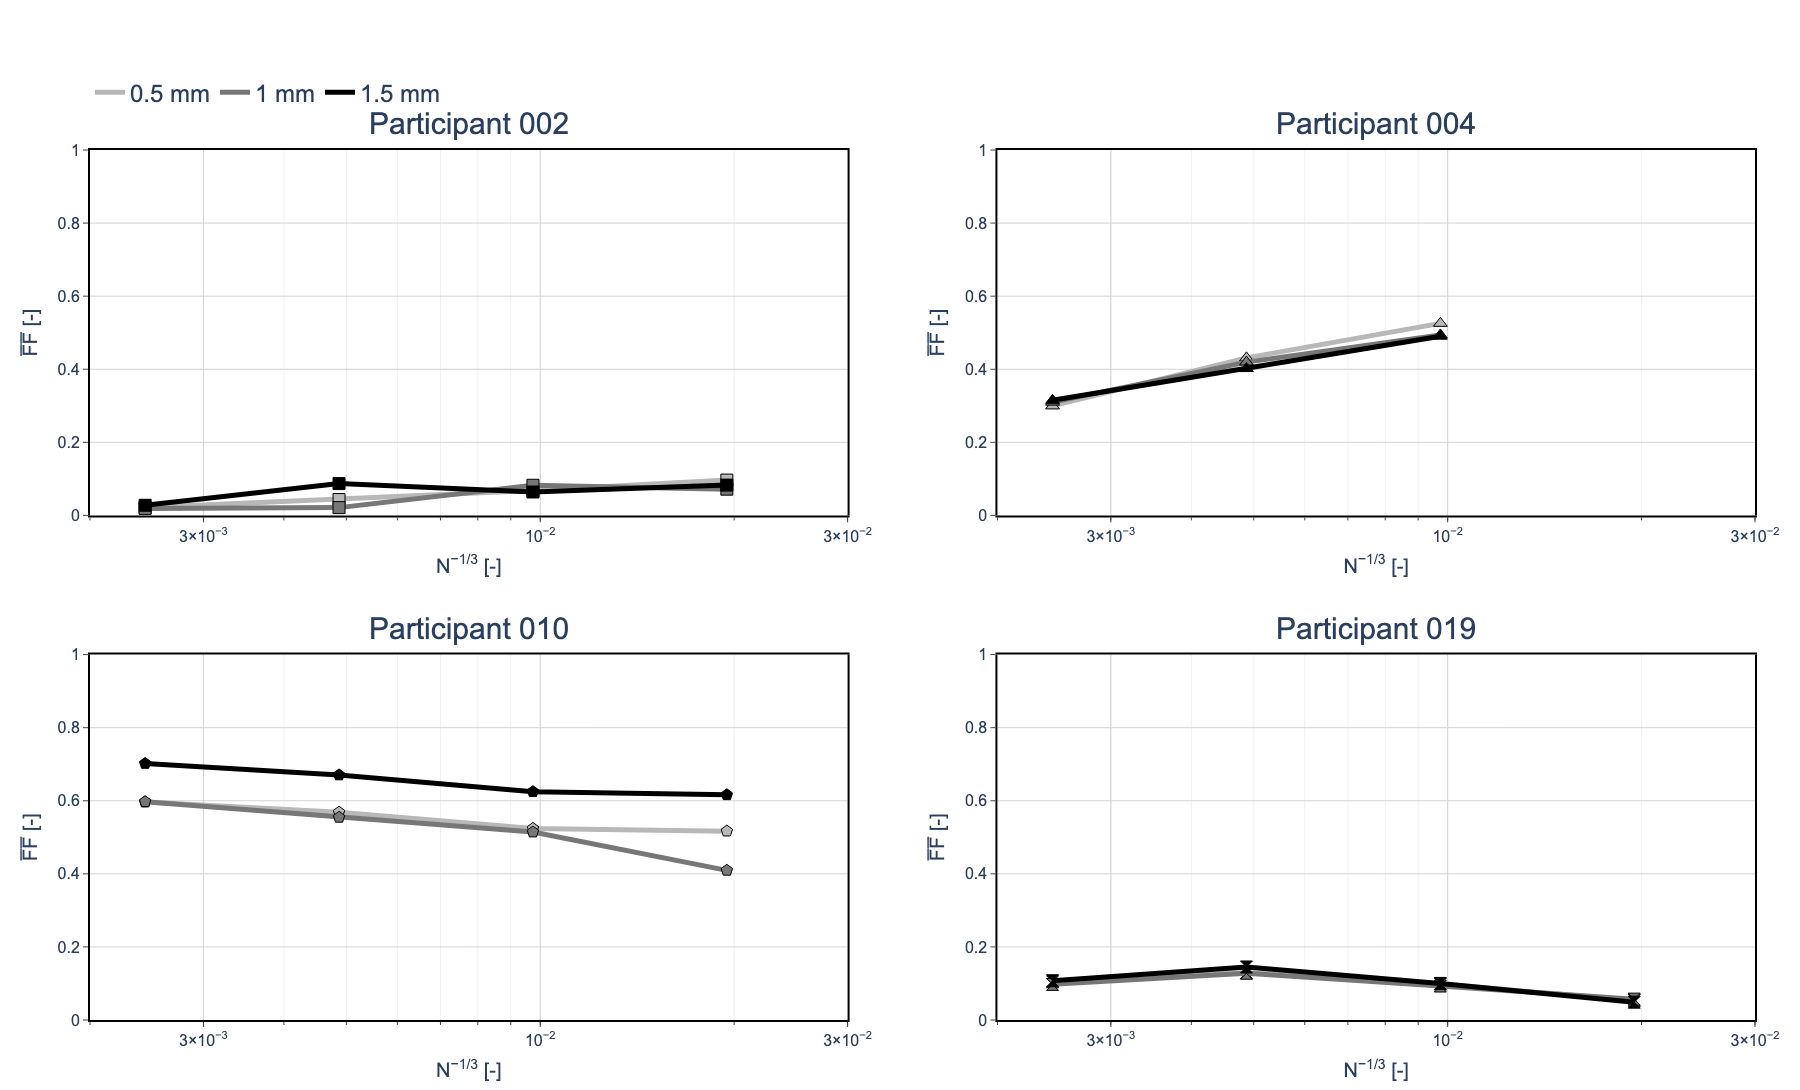
\includegraphics[width=0.8\textwidth]{FIGURES/SURF_TEMP_FF/tc_oneram6_mean_freezing_fraction_vs_n_slice_0p1_grouped_roughness_participants.png}

% \end{frame}

% ============================================================
% ONERA M6 -- Convective Heat Transfer & Thermodynamics Summary
% ============================================================

\begin{frame}{\small ONERA M6 -- Convective Heat Transfer \& Thermodynamics Summary}
\scriptsize

\begin{block}{\scriptsize Convective Heat Transfer}
\begin{itemize}
    \item Considerable code-to-code variability is observed in $HTC$, while reconstructed $T_{\mathrm{rec}}$ distributions remain closely aligned.
    \item Consequently, $Q_c'$ exhibits substantial code-to-code variability, with an L1 IQR of $83.9$ W/m at $y=0.75$ m.
\end{itemize}
\end{block}

\vspace{0.10cm}

\begin{block}{\scriptsize Surface Thermodynamics}
\begin{itemize}
    \item Mean surface temperature shows limited grid sensitivity and comparatively close agreement for most submissions.
    \item In contrast, freezing fraction exhibits larger code-to-code variability in both magnitude and spatial extent.
\end{itemize}
\end{block}

\vspace{0.10cm}

\begin{block}{\scriptsize Roughness Sensitivity}
\begin{itemize}
    \item Increasing roughness consistently increases $HTC$ and $|Q_c'|$.
    \item Mean surface temperature and freezing fraction exhibit code-dependent responses to roughness.
\end{itemize}
\end{block}

\vspace{0.10cm}

\begin{alertblock}{\scriptsize Thermodynamics Takeaway}
Despite consistent aerodynamic loading and $T_{\mathrm{rec}}$, substantial variability develops through the convective and freezing models, with the largest differences appearing in the predicted freezing regime.
\end{alertblock}

\end{frame}




% ============================================================
% ONERA M6 -- ICE ACCRETION
% ============================================================

\section[Ice]{\textbf{Ice Accretion}}

% ============================================================
% ONERA M6 -- Ice Mass Grid Convergence
% ============================================================

\begin{frame}{\small ONERA M6 -- Ice Mass Grid Convergence (15 Bins)}
\scriptsize

\begin{columns}[T,onlytextwidth]

\begin{column}{0.50\textwidth}
    \centering
    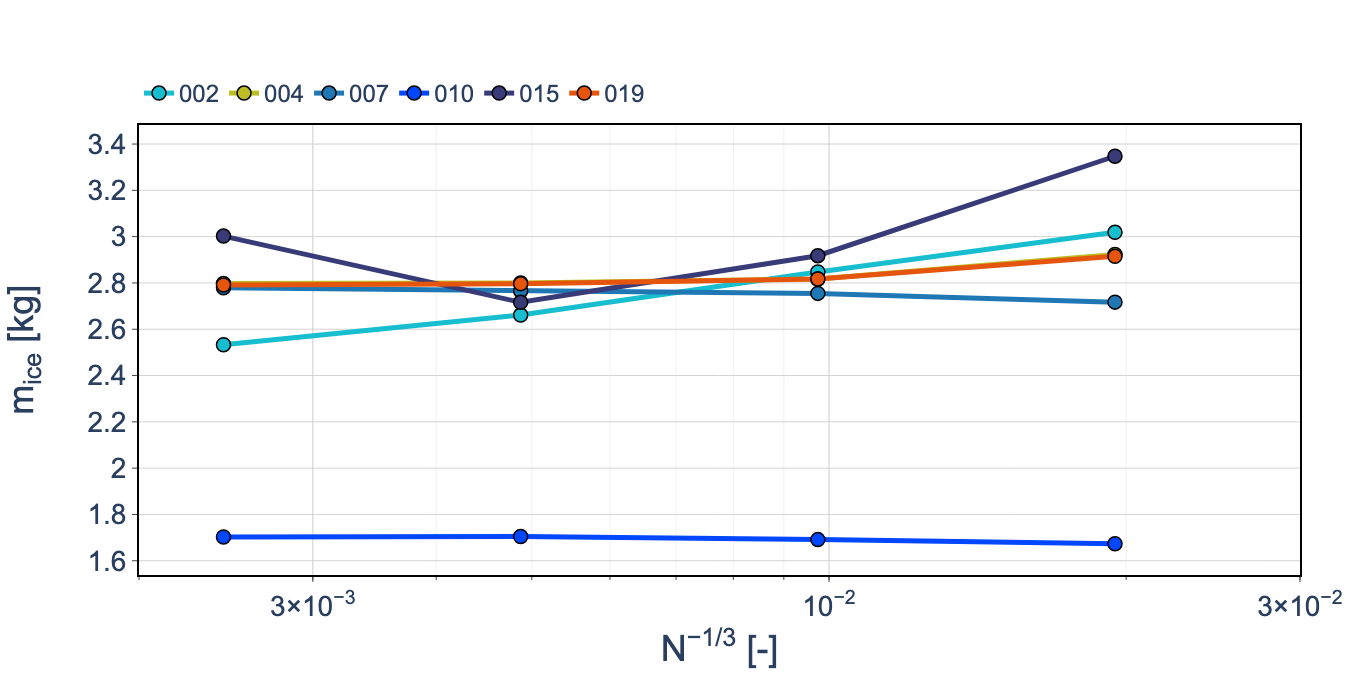
\includegraphics[width=0.94\textwidth]{FIGURES/ICE_ACCRETION/tc_oneram6_ice_mass_vs_n_1mm_bins15_all_grid_levels.png}

    \vspace{0.05cm}

    \textbf{Ice Mass}
\end{column}

\begin{column}{0.50\textwidth}
    \centering
    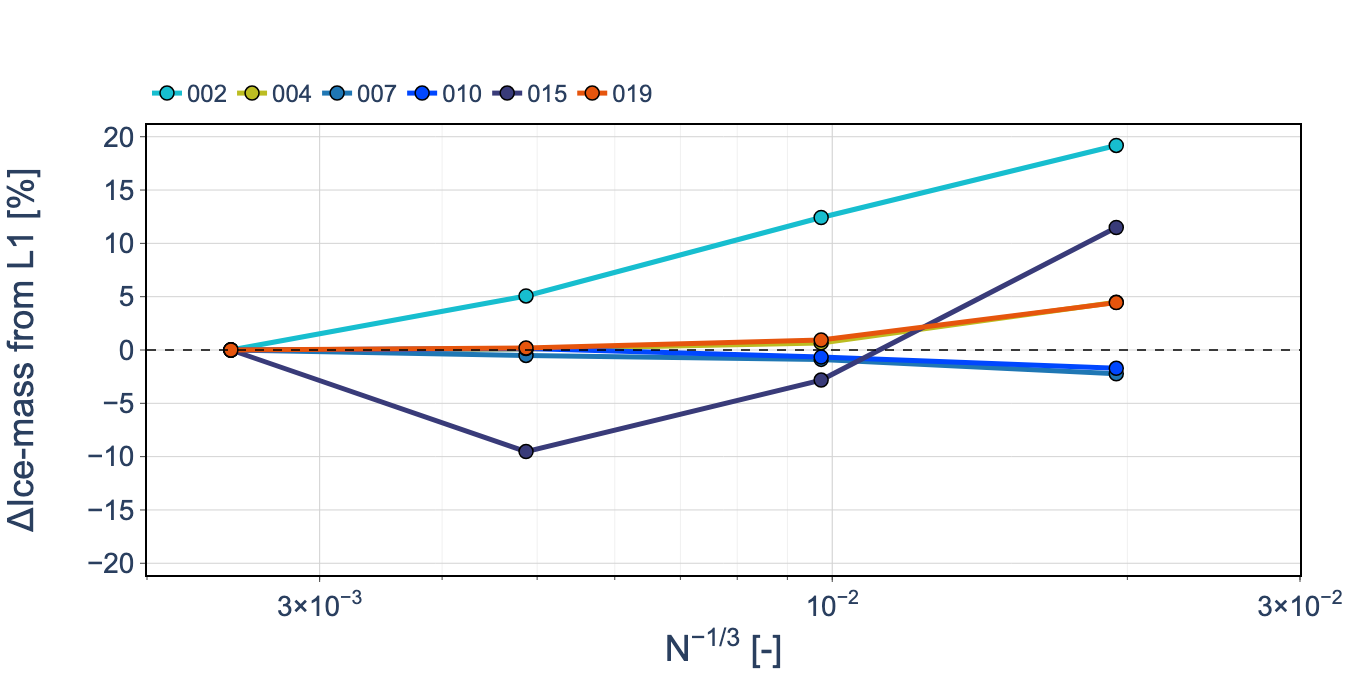
\includegraphics[width=0.94\textwidth]{FIGURES/ICE_ACCRETION/tc_oneram6_ice_mass_vs_n_1mm_bins15_all_grid_levels_relative_to_l1.png}

    \vspace{0.05cm}

    \textbf{Relative to L1}
\end{column}

\end{columns}

\vspace{0.05cm}

{\centering\textbf{Roughness: 1 mm}\par}

\vspace{0.10cm}

\begin{block}{\scriptsize Assessment}
\begin{itemize}
    \item Ice-mass grid sensitivity is strongly submission-dependent.
    \item Relative to L1, coarse-grid differences remain below approximately $5\%$ for several submissions, but reach approximately $20\%$ and $11\%$ for selected submissions on L4.
    \item Considerable code-to-code differences remain on L1 and are generally larger than the grid-refinement effect.
\end{itemize}
\end{block}

\end{frame}


% ============================================================
% ONERA M6 -- Ice Mass Droplet-Distribution Sensitivity
% ============================================================

\begin{frame}{\small ONERA M6 -- Ice Mass Sensitivity to Droplet Distribution}
\scriptsize

\begin{columns}[T,onlytextwidth]

\begin{column}{0.50\textwidth}
    \centering
    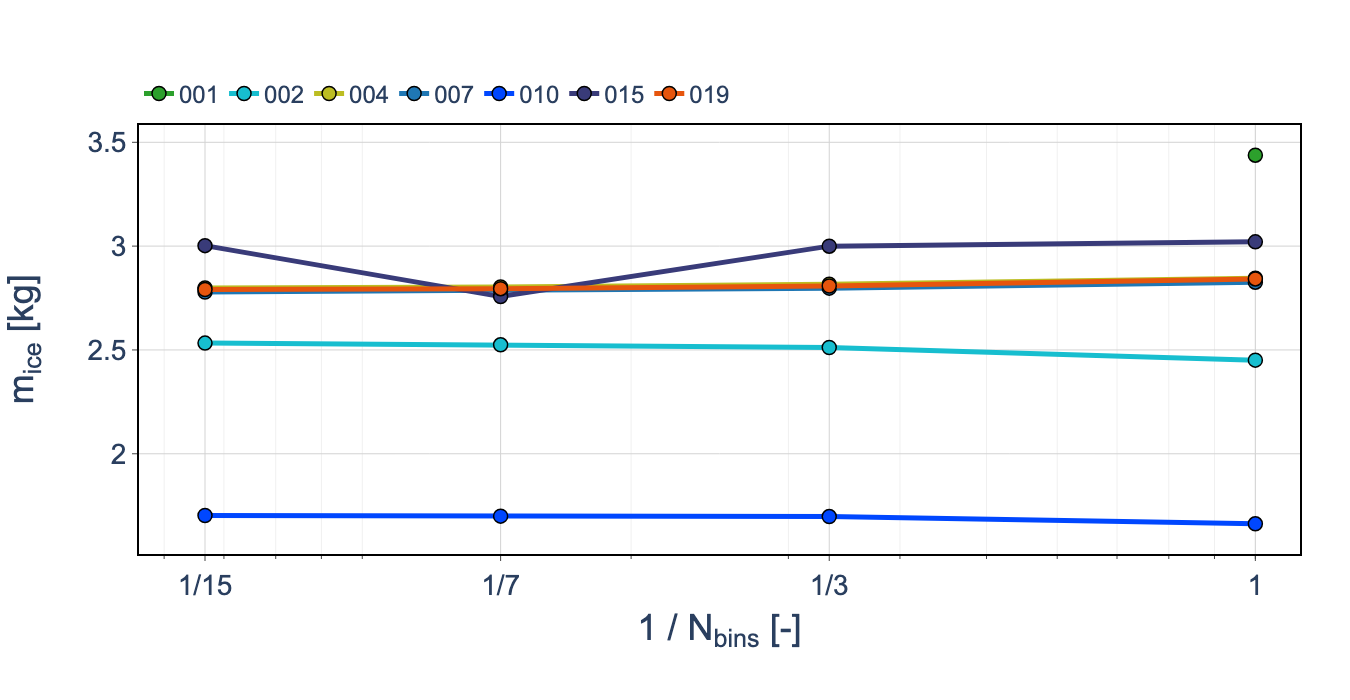
\includegraphics[width=0.94\textwidth]{FIGURES/ICE_ACCRETION/tc_oneram6_ice_mass_vs_n_1mm_l1_vs_inverse_bins.png}

    \vspace{0.05cm}

    \textbf{Ice Mass}
\end{column}

\begin{column}{0.50\textwidth}
    \centering
    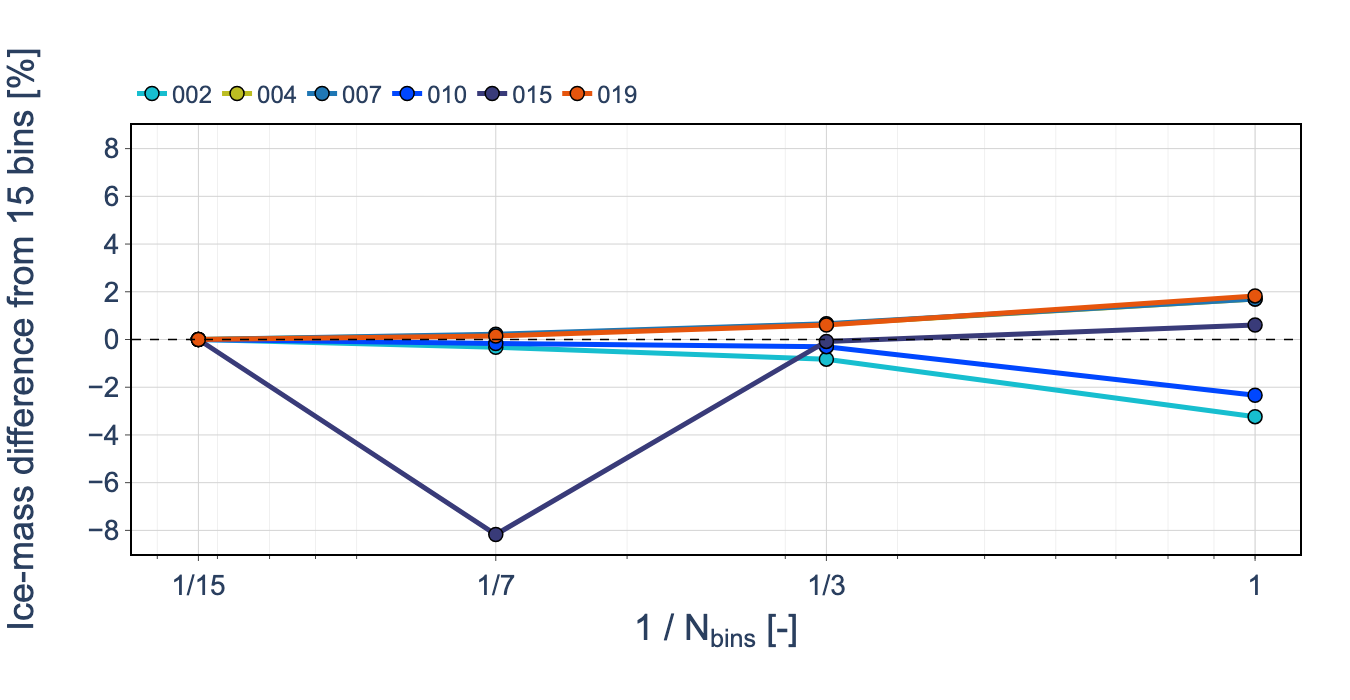
\includegraphics[width=0.94\textwidth]{FIGURES/ICE_ACCRETION/tc_oneram6_ice_mass_vs_n_1mm_l1_vs_inverse_bins_relative_to_bins15.png}

    \vspace{0.05cm}

    \textbf{Relative to 15 Bins}
\end{column}

\end{columns}

\vspace{0.05cm}

{\centering\textbf{L1 -- Roughness: 1 mm}\par}

\vspace{0.10cm}

\begin{block}{\scriptsize Assessment}
\begin{itemize}
    \item Ice mass exhibits limited sensitivity to droplet-distribution resolution for most submissions.
    \item Relative differences from the 15-bin prediction generally remain within approximately $3\%$, with one isolated 7-bin deviation of approximately $8\%$.
    \item Code-to-code differences remain considerably larger than the droplet-distribution effect.
    \item This behavior is consistent with the weak distribution sensitivity previously observed for the integrated impinged water mass.
\end{itemize}
\end{block}

\end{frame}


% ============================================================
% ONERA M6 -- Ice and Evaporation Mass Ratios
% ============================================================

\begin{frame}{\small ONERA M6 -- Ice and Evaporation Mass Ratios}
\scriptsize

\begin{columns}[T,onlytextwidth]

\begin{column}{0.50\textwidth}
    \centering
    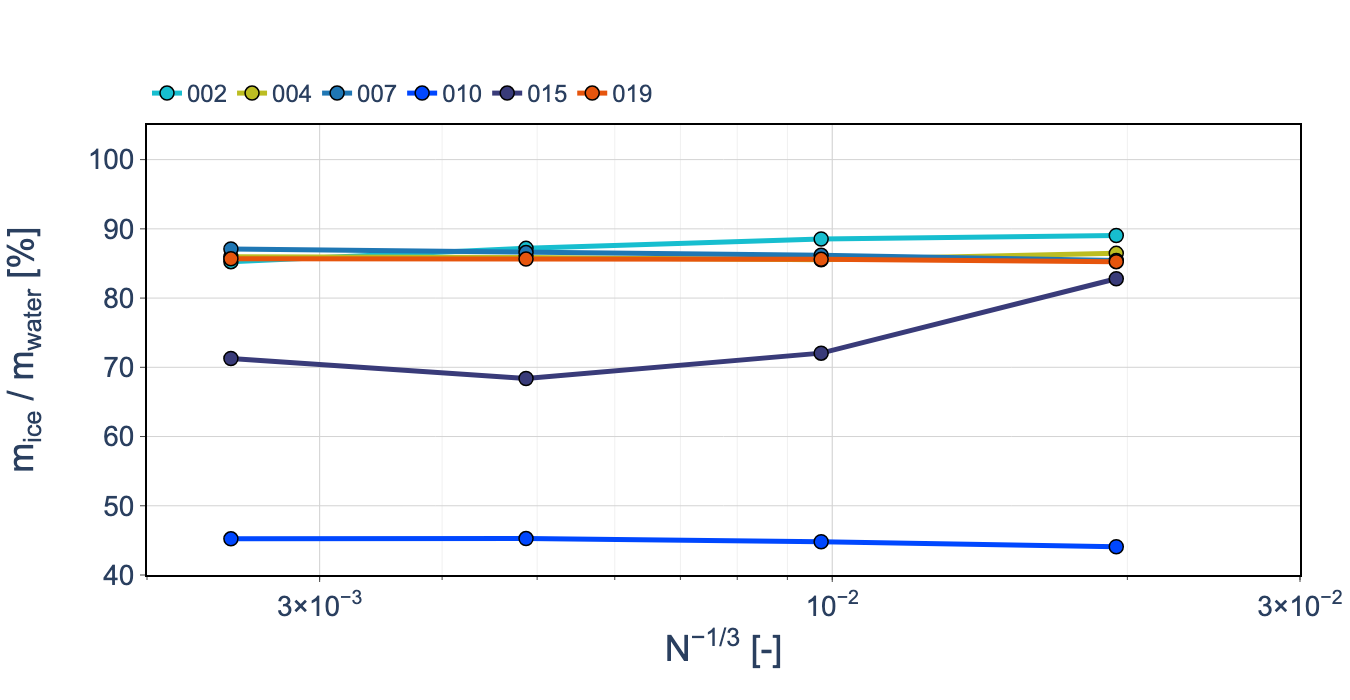
\includegraphics[width=\textwidth]{FIGURES/ICE_ACCRETION/tc_oneram6_ice_to_water_ratio_vs_n_required_bins15.png}

    \vspace{0.05cm}

    {\scriptsize\textbf{Ice / Water}}
\end{column}

\begin{column}{0.50\textwidth}
    \centering
    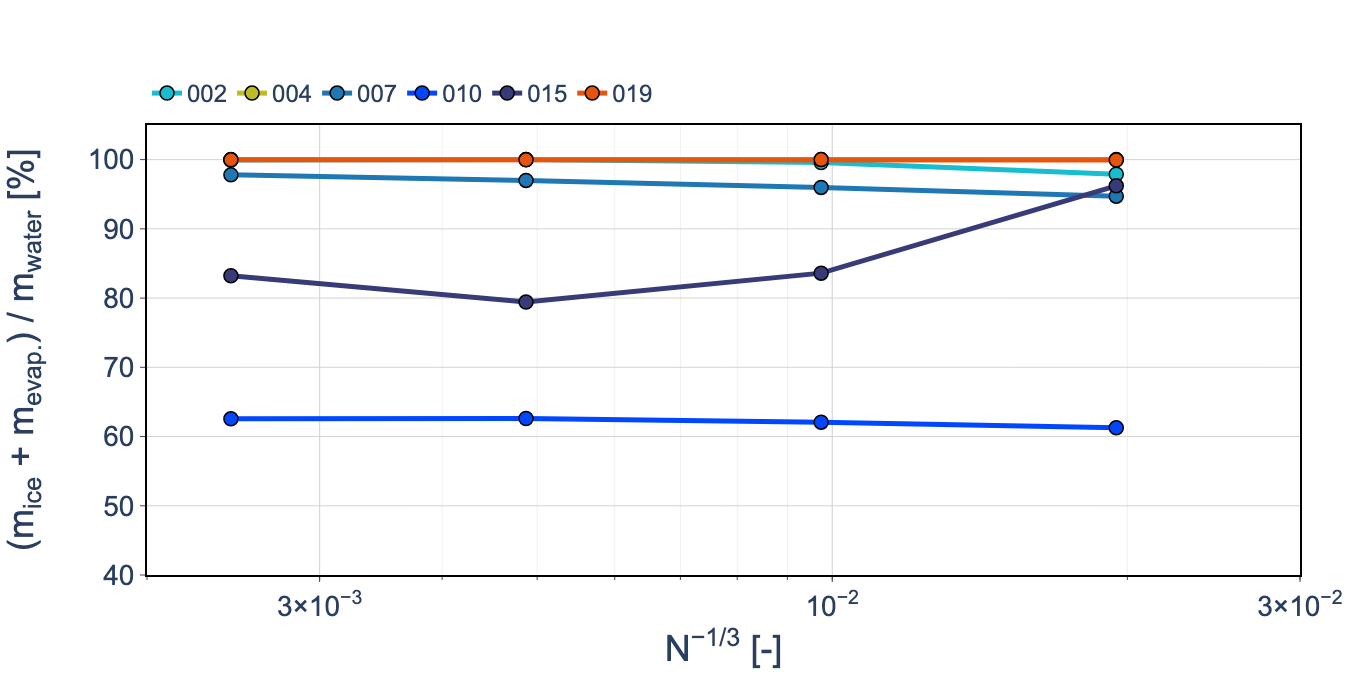
\includegraphics[width=\textwidth]{FIGURES/ICE_ACCRETION/tc_oneram6_ice_evap_to_water_ratio_vs_n_required_bins15.png}

    \vspace{0.05cm}

    {\scriptsize\textbf{(Ice + Evaporation) / Water}}
\end{column}

\end{columns}

\vspace{0.15cm}

\begin{block}{\scriptsize Assessment}
\begin{itemize}
    \item Most submissions convert approximately $85$--$89\%$ of the impinged water mass into ice.
    \item Accounting for evaporation brings the mass balance close to $100\%$ for several submissions, indicating that evaporation explains a significant fraction of the non-accreted water.
    \item Lower ratios for some submissions are consistent with reported water shedding, which provides an additional pathway for the impinged water mass.
\end{itemize}
\end{block}

\end{frame}


% ============================================================
% ONERA M6 -- Ice Mass Roughness Sensitivity
% ============================================================

\begin{frame}{\small ONERA M6 -- Ice Mass Roughness Sensitivity}
\scriptsize

\centering

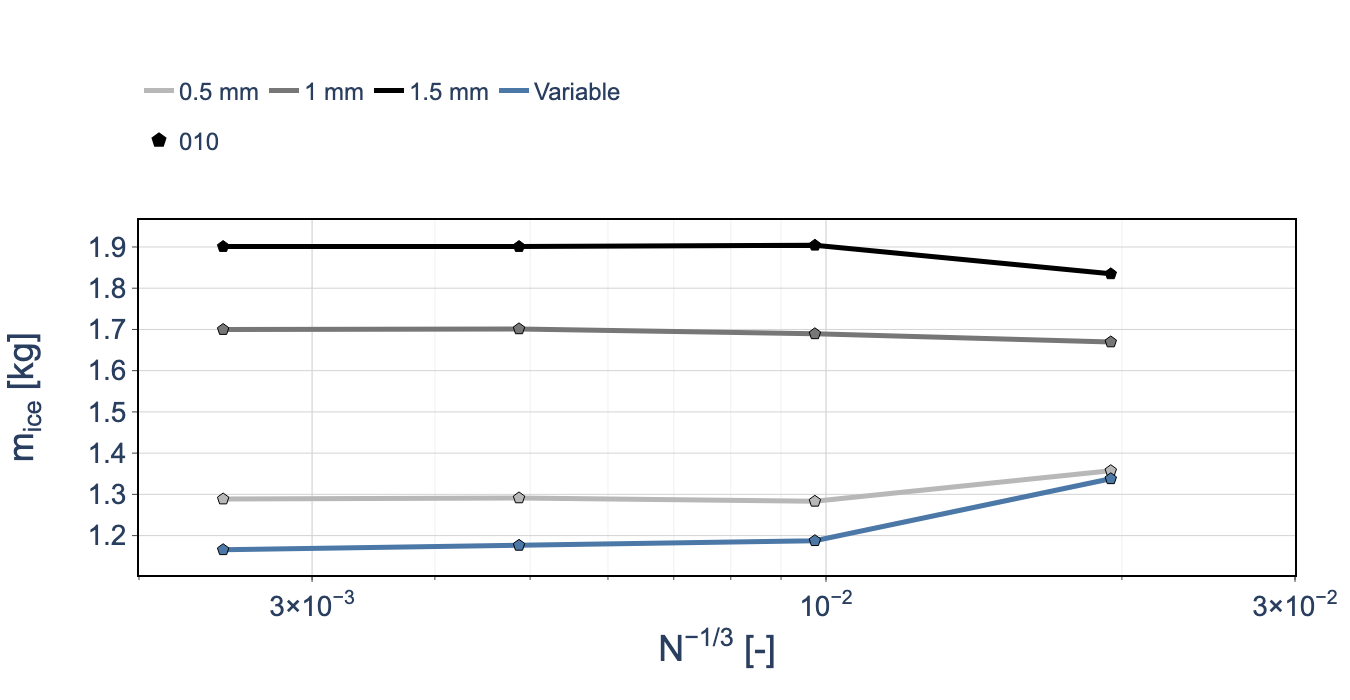
\includegraphics[width=0.70\textwidth]{FIGURES/ICE_ACCRETION/tc_oneram6_010_ice_mass_vs_n_bins07_grouped_roughness.png}

\vspace{0.10cm}

\begin{block}{\scriptsize Assessment}
\begin{itemize}
    \item One submission provided additional results for multiple prescribed roughness heights.
    \item Ice mass increases substantially with roughness, from approximately $1.3$ kg at $k_s=0.5$ mm to $1.9$ kg at $k_s=1.5$ mm on L1.
\end{itemize}
\end{block}

\end{frame}


% ============================================================
% ONERA M6 -- Ice Shapes
% ============================================================

\begin{frame}{\small ONERA M6 -- Ice Shapes (L1, 15 Bins)}
\scriptsize

% ------------------------------------------------------------
% Representative mid-span slice
% ------------------------------------------------------------
\only<1>{

\centering

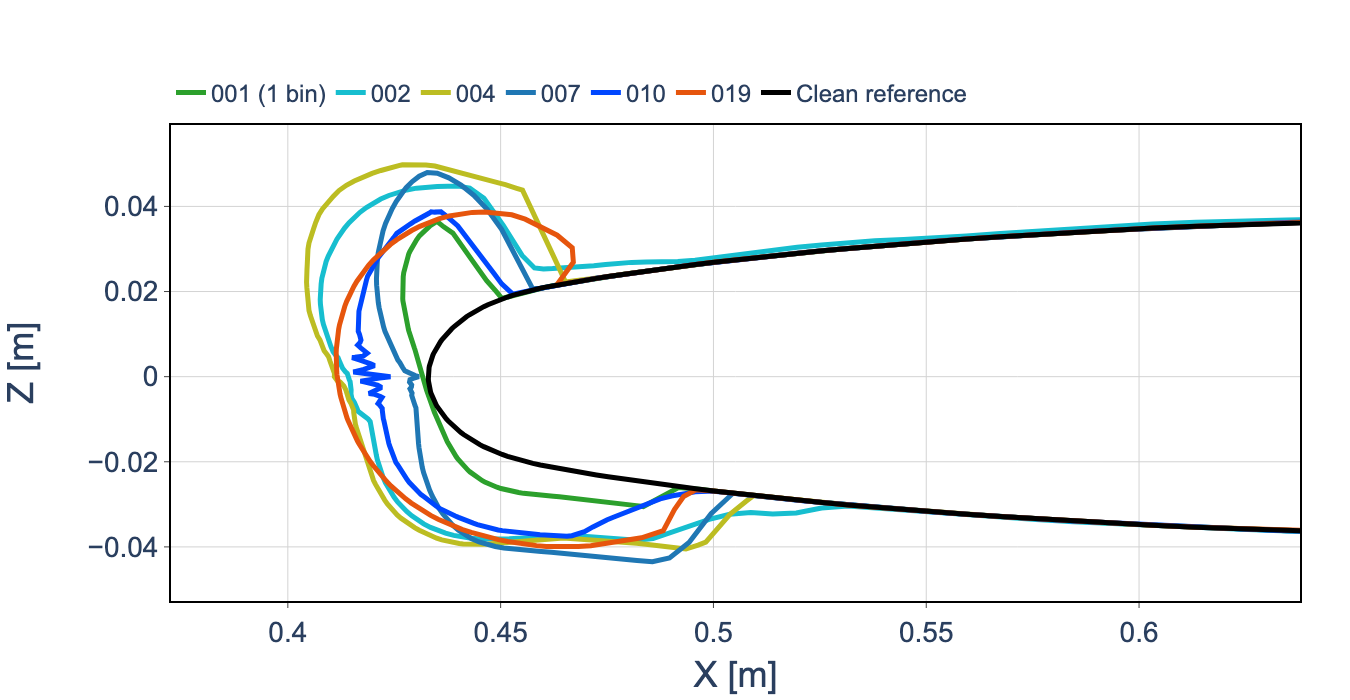
\includegraphics[width=0.6\textwidth]{FIGURES/ICE_SHAPES/tc_oneram6_L1_single_layer_ice_shape_slice_0p75_bins15_roughness_1mm.png}

\vspace{0.05cm}

{\scriptsize\textbf{$y=0.75$ m -- Roughness: 1 mm}}

}

% ------------------------------------------------------------
% Other spanwise slices
% ------------------------------------------------------------
\only<2>{

\begin{columns}[T,onlytextwidth]

\begin{column}{0.50\textwidth}
    \centering

    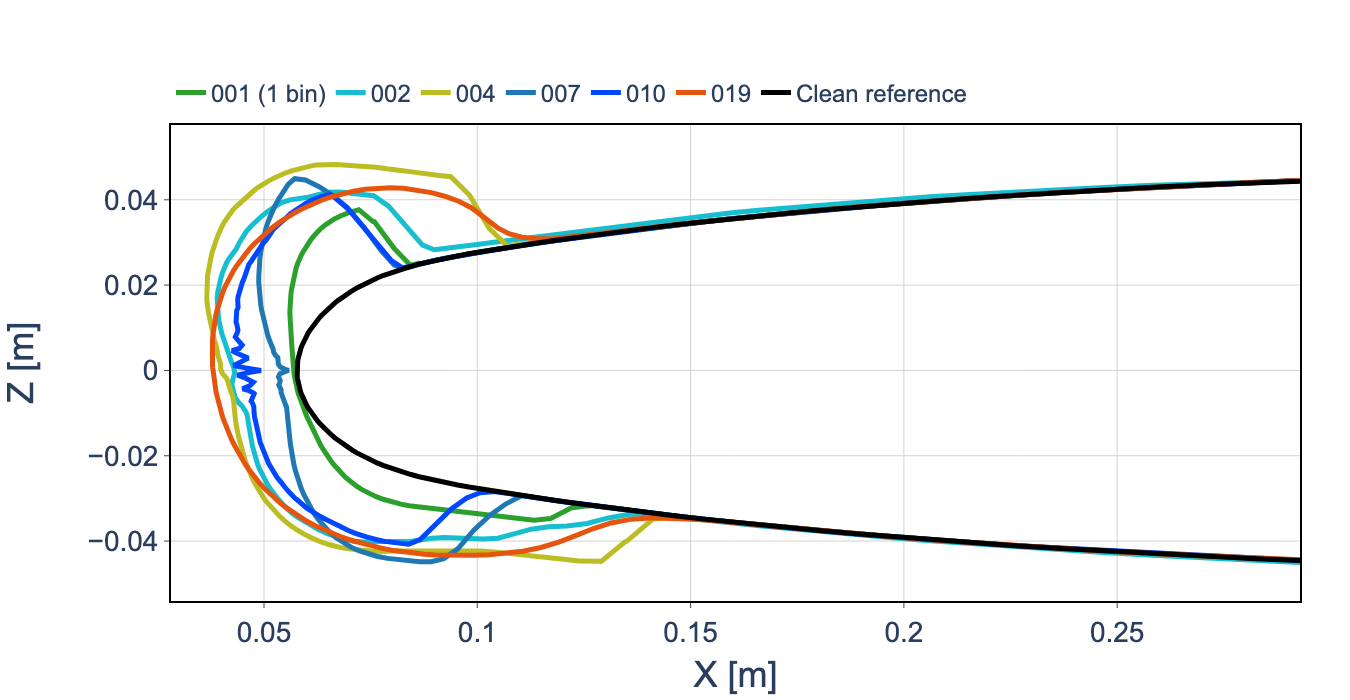
\includegraphics[width=\textwidth]{FIGURES/ICE_SHAPES/tc_oneram6_L1_single_layer_ice_shape_slice_0p1_bins15_roughness_1mm.png}

    \vspace{0.05cm}

    {\scriptsize\textbf{$y=0.10$ m}}
\end{column}

\begin{column}{0.50\textwidth}
    \centering

    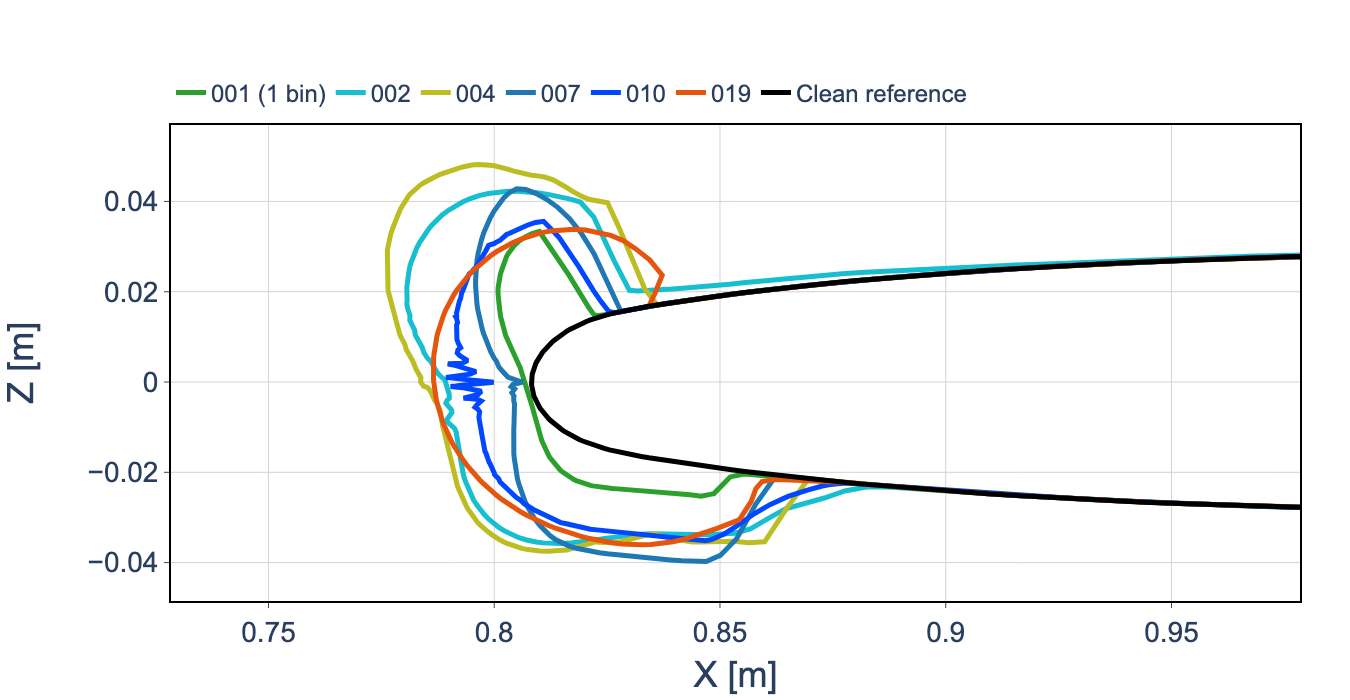
\includegraphics[width=\textwidth]{FIGURES/ICE_SHAPES/tc_oneram6_L1_single_layer_ice_shape_slice_1p4_bins15_roughness_1mm.png}

    \vspace{0.05cm}

    {\scriptsize\textbf{$y=1.40$ m}}
\end{column}

\end{columns}

}

\vspace{0.15cm}

\begin{block}{\scriptsize Assessment}
\begin{itemize}
    \item Considerable code-to-code variability is observed in the predicted ice shape, particularly in horn height, orientation, and local accretion thickness.
    \item Despite these differences, the submissions predict a broadly similar overall accretion region around the leading edge.
    \item<2-> Similar code-to-code variability is observed at the other spanwise locations.
    \item<2-> The geometric spread is consistent with the differences previously observed in the thermodynamic predictions, despite comparatively good agreement in water impingement.
\end{itemize}
\end{block}

\end{frame}

% ============================================================
% ONERA M6 -- Multilayer Ice Shapes
% ============================================================

\begin{frame}{\small ONERA M6 -- Multilayer Ice-Shape Comparison}
\scriptsize

% ------------------------------------------------------------
% Middle slice
% ------------------------------------------------------------
\only<1>{
\centering
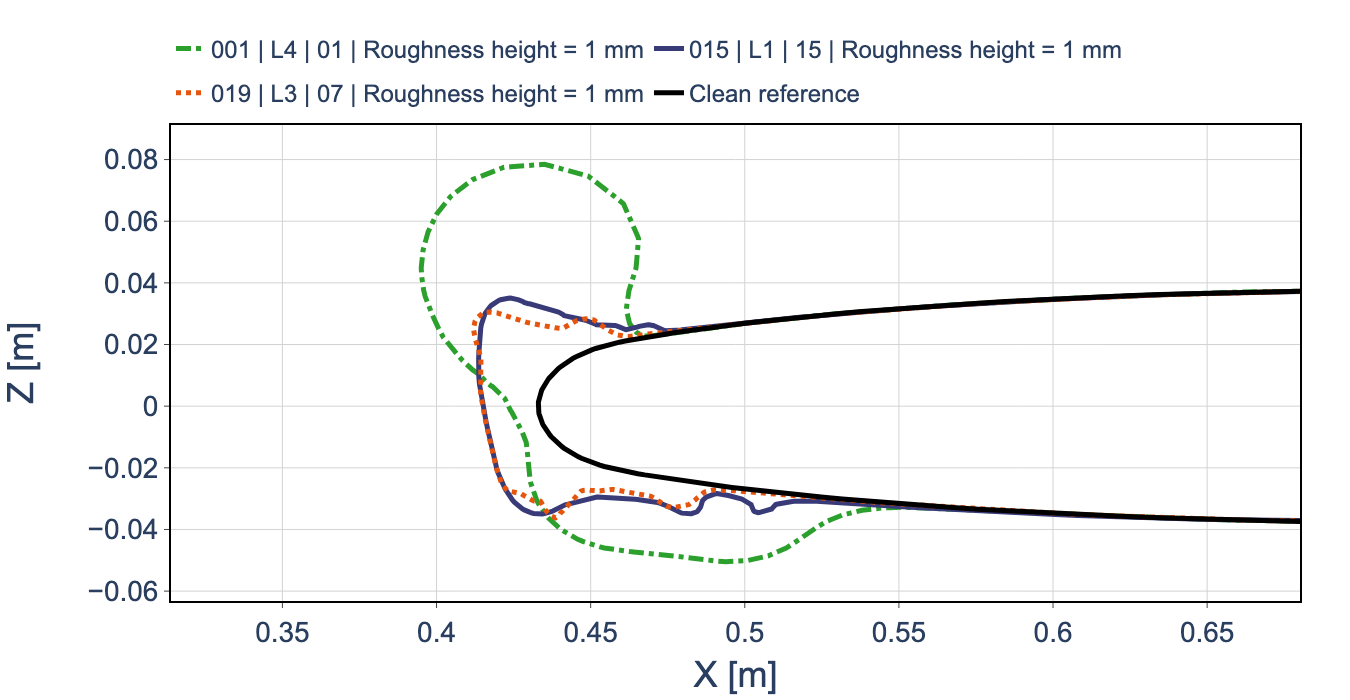
\includegraphics[width=0.70\textwidth]{FIGURES/ICE_SHAPES/tc_oneram6_finest_grid_multilayer_ice_shape_slice_0p75_all_conditions.png}

\vspace{0.05cm}

\textbf{$y=0.75$ m}
}

% ------------------------------------------------------------
% Inboard and outboard slices
% ------------------------------------------------------------
\only<2>{
\begin{columns}[T,onlytextwidth]

\begin{column}{0.50\textwidth}
    \centering
    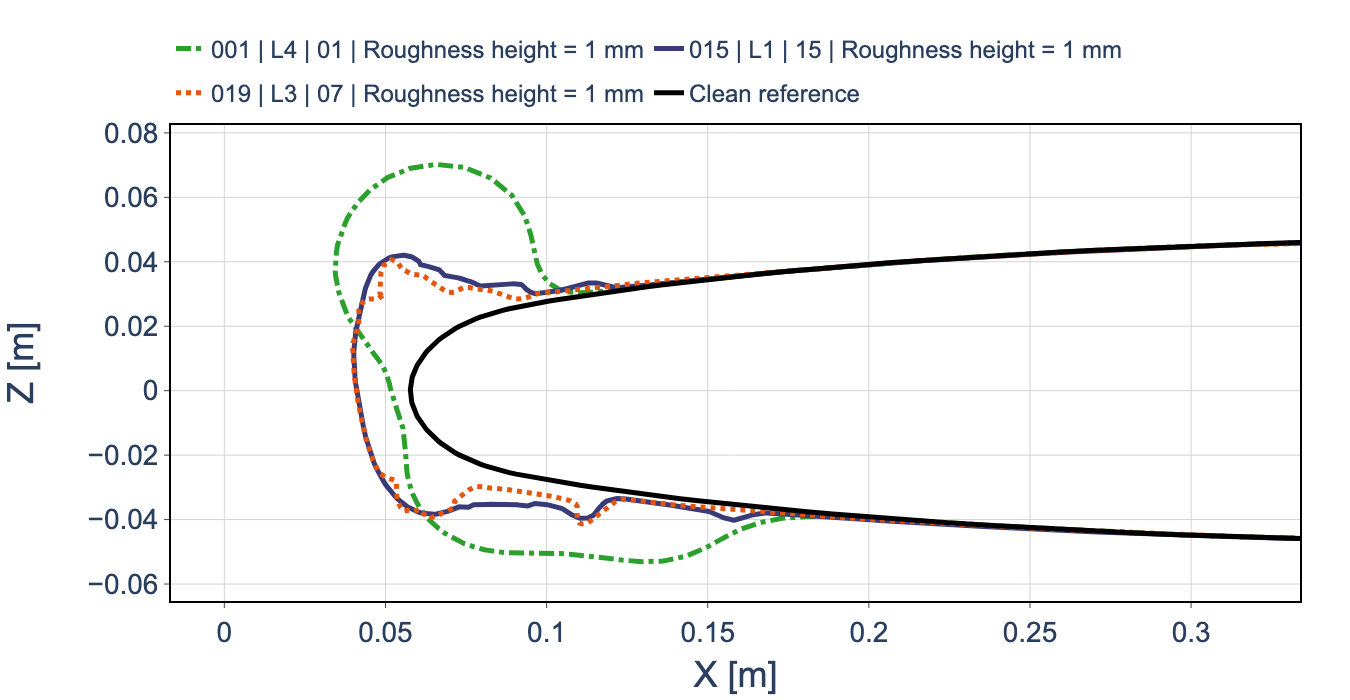
\includegraphics[width=0.94\textwidth]{FIGURES/ICE_SHAPES/tc_oneram6_finest_grid_multilayer_ice_shape_slice_0p1_all_conditions.png}

    \vspace{0.05cm}

    \textbf{$y=0.10$ m}
\end{column}

\begin{column}{0.50\textwidth}
    \centering
    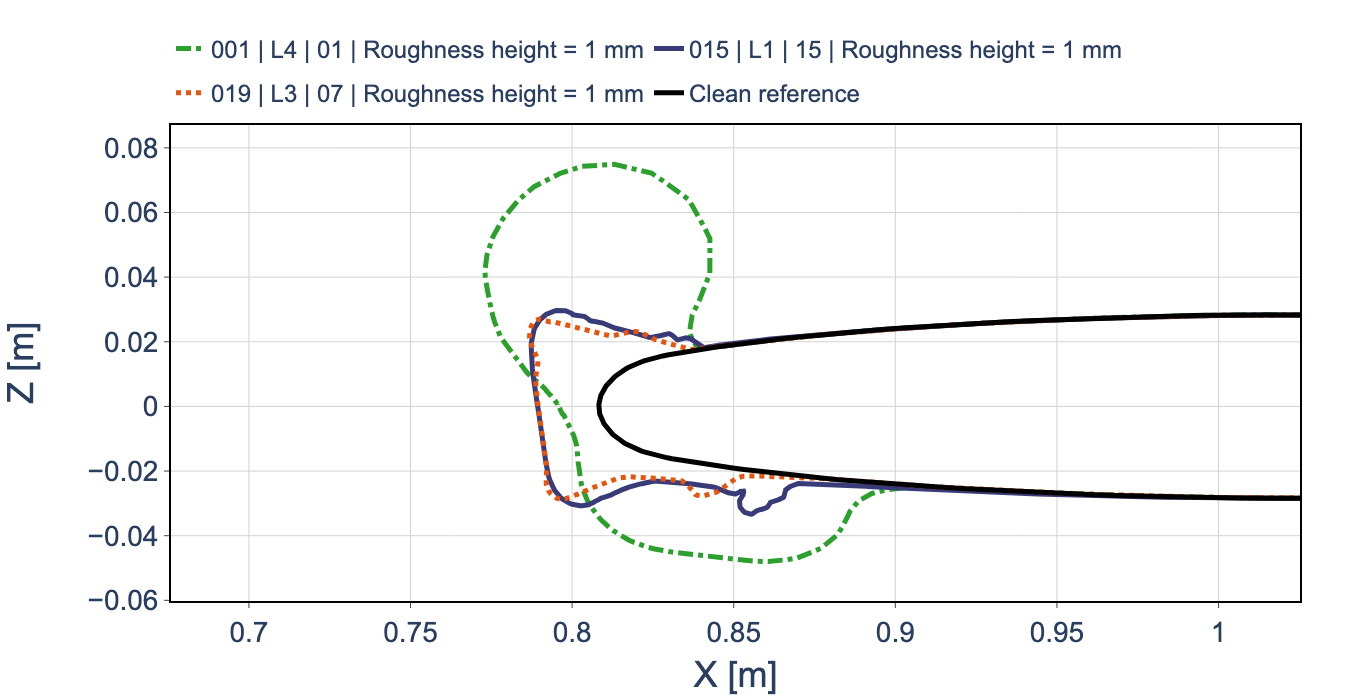
\includegraphics[width=0.94\textwidth]{FIGURES/ICE_SHAPES/tc_oneram6_finest_grid_multilayer_ice_shape_slice_1p4_all_conditions.png}

    \vspace{0.05cm}

    \textbf{$y=1.40$ m}
\end{column}

\end{columns}
}

\vspace{0.10cm}

\begin{block}{\scriptsize Assessment}
\begin{itemize}
    \item<1-> Considerable code-to-code variability is observed in horn orientation, extent, and local ice thickness.
    \item<1-> Predicted accretion ranges from relatively compact shapes to substantially larger upper- and lower-surface horns.
    \item<2-> Similar geometric variability persists at the inboard and outboard spanwise stations.
\end{itemize}
\end{block}

\end{frame}


% ============================================================
% ONERA M6 -- Ice Accretion Summary
% ============================================================

\begin{frame}{\small ONERA M6 -- Ice Accretion Summary}
\scriptsize

\begin{block}{\scriptsize Ice Mass}
\begin{itemize}
    \item Grid sensitivity is submission-dependent, while sensitivity to droplet discretization remains limited.
    \item Code-to-code differences remain substantial and generally exceed the grid and droplet-discretization effects.
\end{itemize}
\end{block}

\vspace{0.08cm}

\begin{block}{\scriptsize Mass Partition}
\begin{itemize}
    \item Most submissions convert approximately $85$--$89\%$ of the impinged water mass into ice.
    \item Evaporation closes much of the remaining mass balance; lower ratios for some submissions are consistent with reported water shedding.
\end{itemize}
\end{block}

\vspace{0.08cm}

\begin{block}{\scriptsize Ice Geometry}
\begin{itemize}
    \item Considerable code-to-code variability is observed in horn height, orientation, and local ice thickness.
    \item Similar geometric variability persists across the three spanwise sections.
\end{itemize}
\end{block}

\vspace{0.08cm}

\begin{alertblock}{\scriptsize Ice Accretion Takeaway}
Good agreement in water impingement does not translate into comparable ice accretion; substantial differences emerge in mass partition and final ice geometry, highlighting the influence of the thermodynamic treatment.
\end{alertblock}

\end{frame}

% ============================================================
% ============================================================
% ONERA M6 -- OVERALL ASSESSMENT
% ============================================================
% ============================================================

\section[Overview]{\textbf{ONERA M6 Overall Assessment}}

% ============================================================
% ONERA M6 -- Overall Assessment
% ============================================================

\begin{frame}{\small ONERA M6 -- Overall Assessment}
\scriptsize

\begin{block}{\scriptsize Overall Assessment}
\begin{itemize}
    \item \textbf{Aerodynamics:} Limited grid and code-to-code variability overall, except for $C_D$.
    \item \textbf{Droplet Impingement:} Good overall agreement; impingement extent is more sensitive to spatial and droplet-distribution resolution than integrated water mass.
    \item \textbf{HTC \& Thermodynamics:} Substantial code-to-code variability, particularly in $HTC$, convective heat transfer, and freezing fraction.
    \item \textbf{Ice Accretion:} Comparable water impingement does not translate into comparable ice mass or final ice geometry.
\end{itemize}
\end{block}

\vspace{0.10cm}

\begin{alertblock}{\scriptsize Overall Takeaway}
Code-to-code variability increases through the icing simulation chain, with large differences emerging in thermodynamics and final ice accretion. HTC and thermodynamic modeling deserve closer investigation for these glaze conditions, while geometry-evolution methods also clearly influence the final ice shape, even when thermodynamic predictions are comparable.
\end{alertblock}

\end{frame}

\end{document}
